\documentclass[oneside]{book}

\usepackage[utf8]{inputenc}
\usepackage{amsthm}
\usepackage{amssymb}
\usepackage{amsmath}
\usepackage{dsfont}
\usepackage{xcolor}
\usepackage{natbib}
\usepackage{enumitem}
\usepackage{verbatim}
\usepackage{lipsum}
\usepackage{tikz}
\usepackage{mathtools}
\usepackage{float}
\usepackage{graphicx}
\usepackage{subfig}
\usepackage{wrapfig}

\usepackage{hyperref}
\hypersetup{
    colorlinks,
    citecolor=black,
    filecolor=black,
    linkcolor=black,
    urlcolor=black
}
    
\graphicspath{{"/Users/Johannes/Documents/TeX/Speciale/report/images/"}}
\captionsetup[subfigure]{labelformat=empty}

% Theorem enviroments, which all use the same counter
\theoremstyle{definition}
\newtheorem{thm}{Theorem}
\newtheorem{defn}[thm]{Definition}
\newtheorem{cor}[thm]{Corollary}
\newtheorem{lem}[thm]{Lemma}
\newtheorem{prop}[thm]{Proposition}
\newtheorem{ex}[thm]{Example}
\newtheorem{rmk}[thm]{Remark}
\newtheorem{calc}[thm]{Calculation}
\numberwithin{thm}{chapter}
%\numberwithin{equation}{section}

\numberwithin{equation}{chapter}
\renewcommand{\theequation}{\thechapter.\arabic{equation}}

% Sets
\newcommand{\R}{\mathbb{R}}
\newcommand{\F}{\mathbb{F}}
\newcommand{\N}{\mathbb{N}}
\newcommand{\Z}{\mathbb{Z}}

% Misc
\newcommand{\curly}[1]{\{#1\}}
\newcommand{\abs}[1]{\left\lvert #1 \right\rvert}
\newcommand{\norm}[1]{\left\lVert #1 \right\rVert}
\newcommand{\ip}[2]{\left\langle #1, #2 \right\rangle}
\newcommand{\para}[1]{\left(#1\right)}
\newcommand{\makeset}[2]{\curly{#1 \mid #2}}

% Todo
\newcommand{\todo}[1]{{\color{red} (\textsc{todo}: #1)}}
\newcommand{\ques}[1]{{\color{red} (\textsc{question}: #1)}}

% CompGeo
\DeclareMathOperator{\dist}{dist}
\DeclareMathOperator{\Vor}{Vor}
\DeclareMathOperator{\bi}{bi}

\begin{document}

\begin{titlepage}
\begin{center}
\Huge{\textsc{Computing Voronoi Diagrams Using Fortune's Algorithm}}

\par
\vspace{0.6cm}

\Large{\textsc{Student: Johannes Jensen, 201505594}}

\par
\vspace{0.33cm}

\Large{\textsc{Supervisor: Gerth Stølting Brodal}}

\par
\vspace{0.33cm}

\large{\textsc{Master Thesis in Mathematics}}
\par
\large{\textsc{Aarhus University}}

\par
\vspace{0.25cm}

\normalsize{\textsc{June 15, 2022}}
\end{center}
\[
    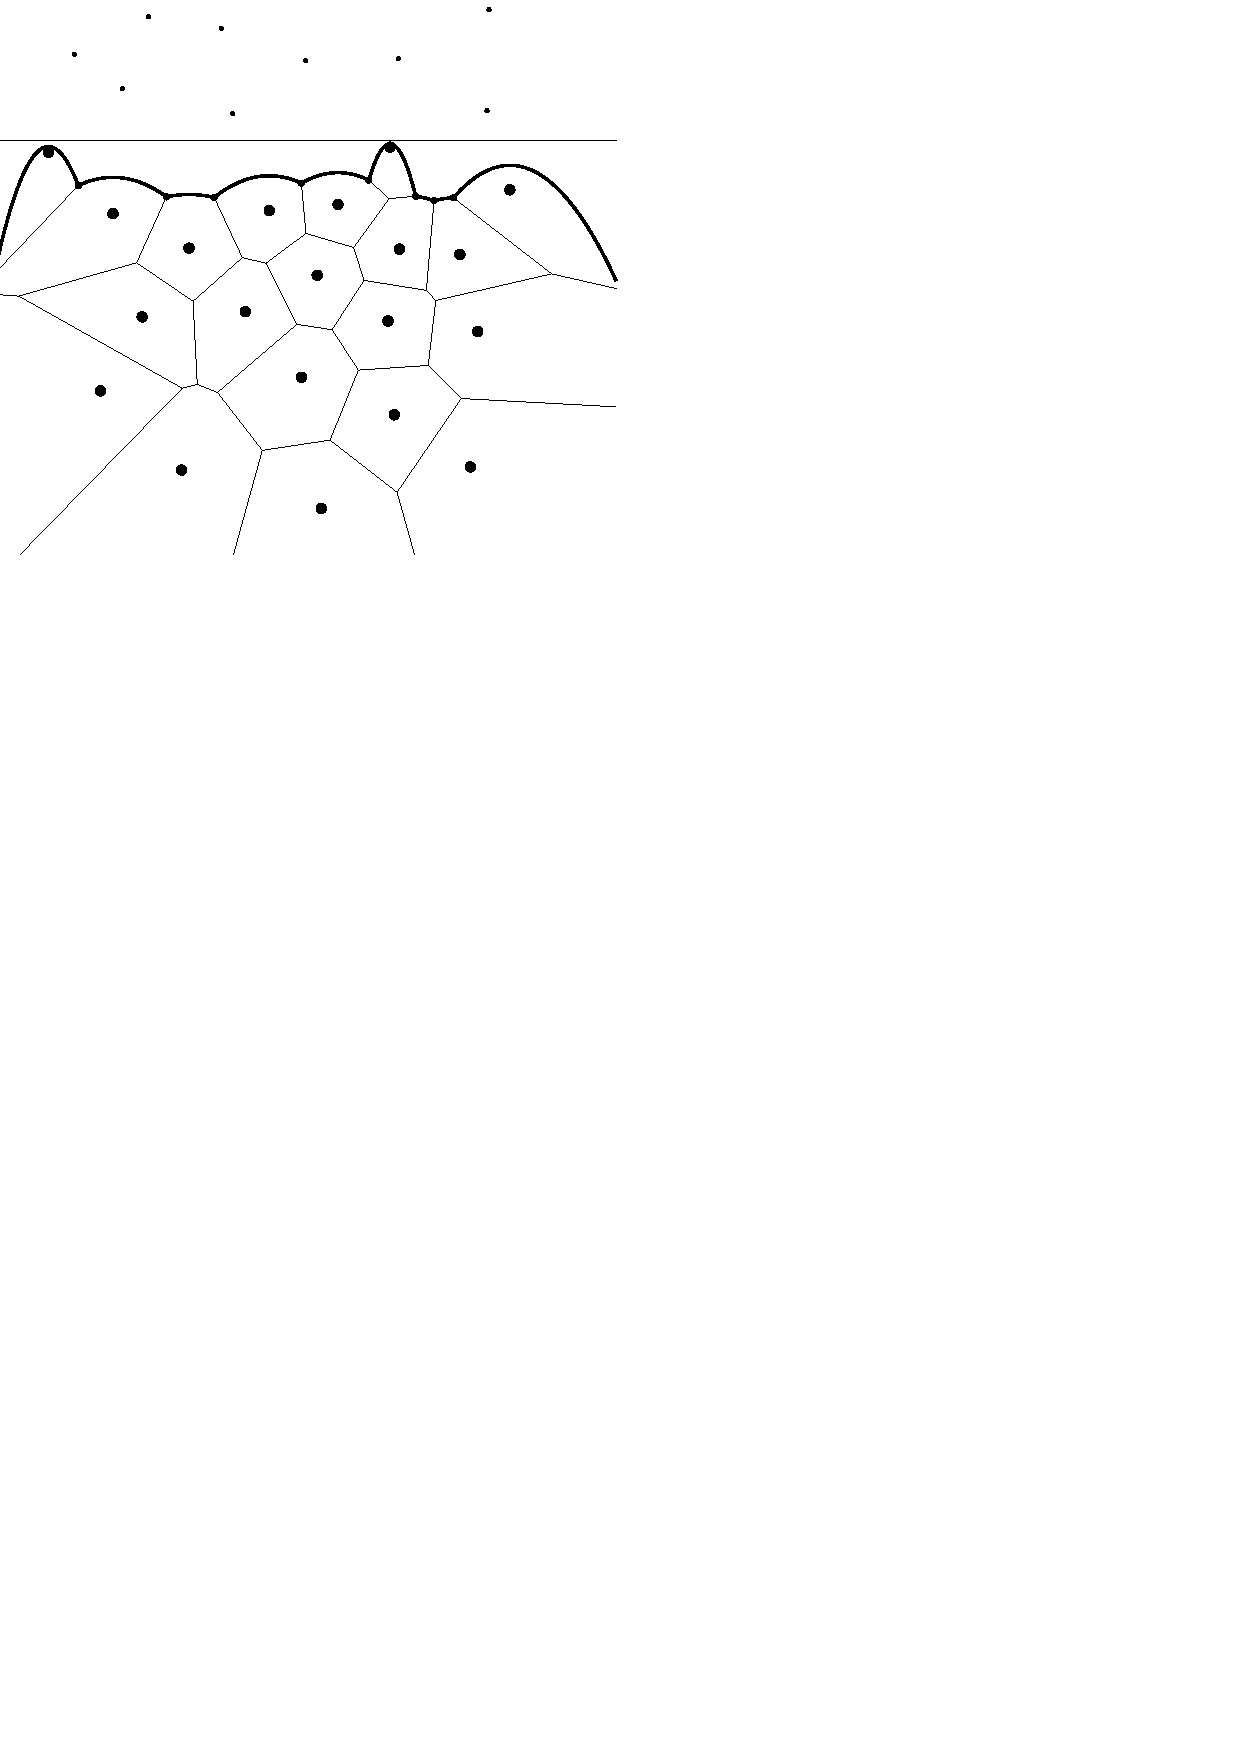
\includegraphics[scale=1.3]{frontpage}
\]

\end{titlepage}

\frontmatter
\chapter{Abstract}

The main goal of this master thesis is to solve the following problem: Given a set of $n$ points $P$ in the plane called sites, draw polygons around the sites such that none of the polygons' interiors overlap, every polygon contains only one site, and such that the distance from every point inside a polygon is closer to the site inside the polygon with respect to the Euclidean distance, than it is to any of the other sites. Such a collection of polygons is called an Euclidean Voronoi diagram for the set of sites $P$.

We will work towards presenting an algorithm which runs in $\mathcal{O}(n \log n)$ time, which is called Fortune's algorithm. This is a sweep line algorithm, which sweeps a hypothetical horizontal line down through the plane, uncovering the structure of the Voronoi diagram along the way.

First we look at some theory, where we prove some local and global properties of Euclidean Voronoi diagrams, and how they interact with the sweep line. Afterwards we describe some data structures that we will use, and during this we will describe and prove some properties about treaps, which are randomized binary search trees. Finally, we put everything together and describe the algorithm in detail.

\tableofcontents

\mainmatter
\chapter{Introduction}

aslkdfj
\chapter{Properties of Euclidean Voronoi Diagrams}

% % % % % % % % % % % % % % % % % % % % % % % % % % % % % % % % % % % %
%
% Definition
%
% % % % % % % % % % % % % % % % % % % % % % % % % % % % % % % % % % % % 
In this chapter we will consider Voronoi diagrams for the $L^2$ norm, also known as the Euclidean norm. The norm is given by
\[
    \norm{(x, y)}_2 = \sqrt{x^2 + y^2},
\]
for all $x, y \in \R$. Here is the example diagram with this norm from earlier:
\begin{figure}[H]
    \centering
    \subfloat{
      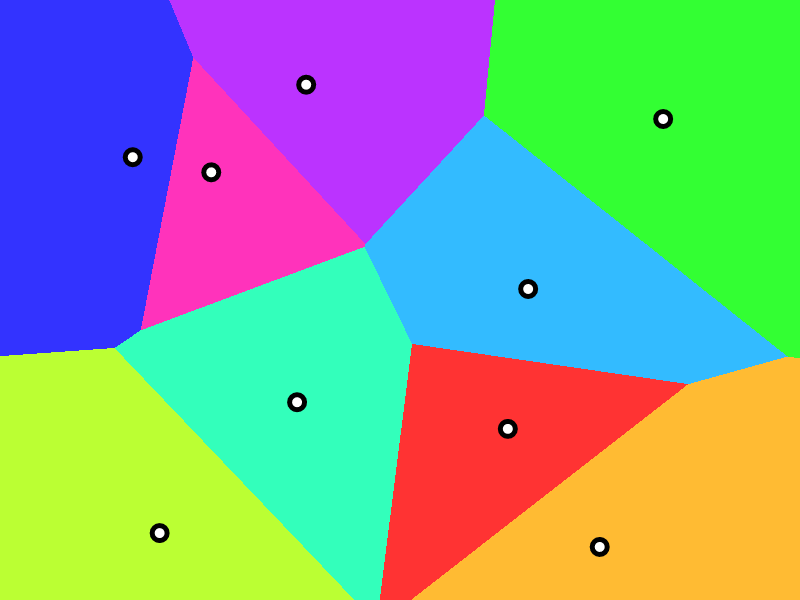
\includegraphics[scale=0.21]{naive-voronoi-L2}
    }
    \subfloat{
      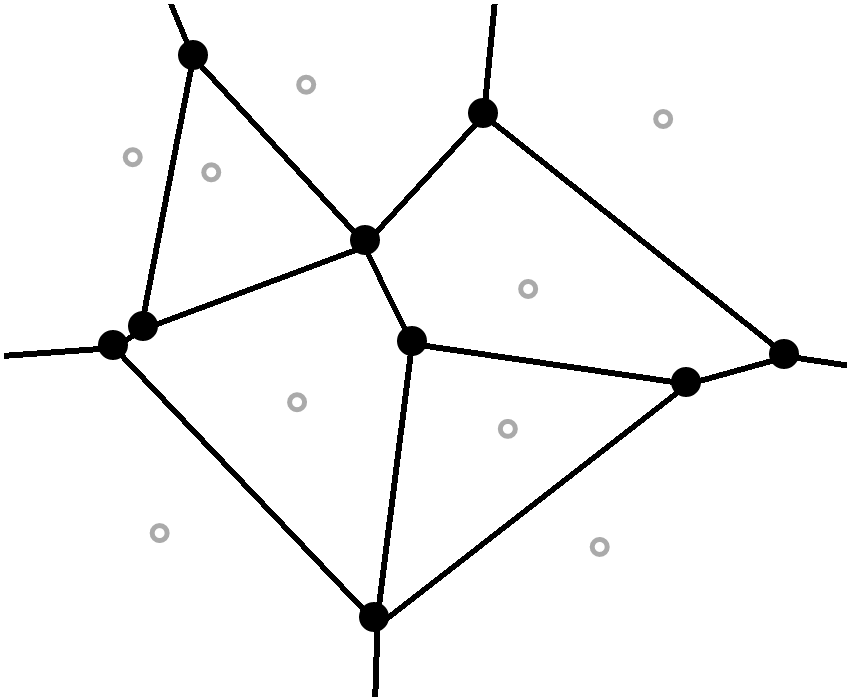
\includegraphics[scale=0.18]{naive-voronoi-graph-L2}
    }
\end{figure}
We note that the diagram consists of straight lines, rays and line segments. In the following sections we will describe the shape of the diagram in detail.

% % % % % % % % % % % % % % % % % % % % % % % % % % % % % % % % % % % %
%
% Preliminary definitions: Bisector, halfplane, Voronoi cells
%
% % % % % % % % % % % % % % % % % % % % % % % % % % % % % % % % % % % % 

\section{Bisectors, halfplanes and Voronoi cells}
From linear algebra we know that $\norm{v}_2 = \sqrt{\ip{v}{v}}$, where $\ip{\,\cdot\,}{\,\cdot\,}$ is the usual dot product on $\R^2$. Given two points $p, q \in \R^2$ then the \textbf{bisector} of $p$ and $q$ is denoted by $\bi(p, q) \subset \R^2$ and denotes the set of points on a line $\ell$ which passes through the midpoint of $p$ and $q$ and is orthogonal (w.r.t. $\ip{\,\cdot\,}{\,\cdot\,}$) to the vector $p - q$.
\[
    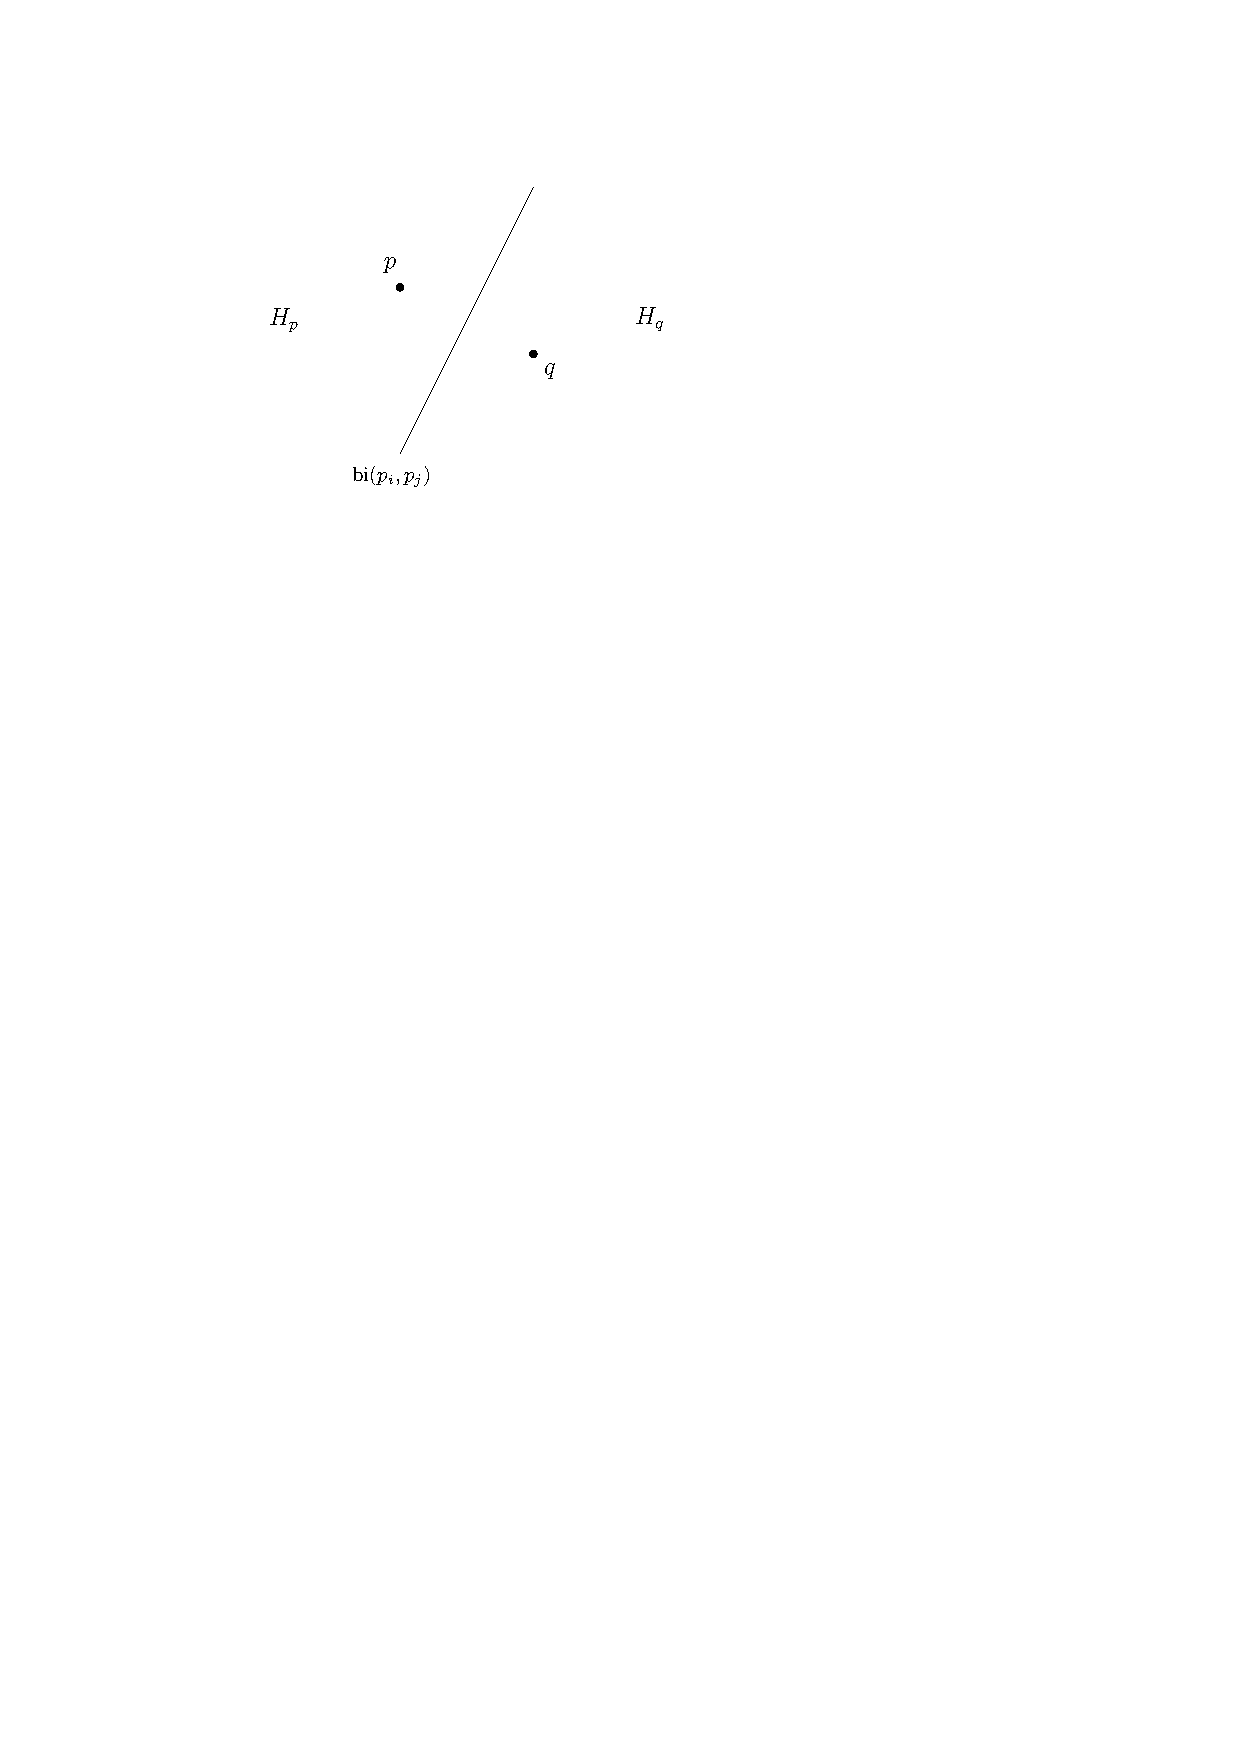
\includegraphics[scale=0.8]{bisector} %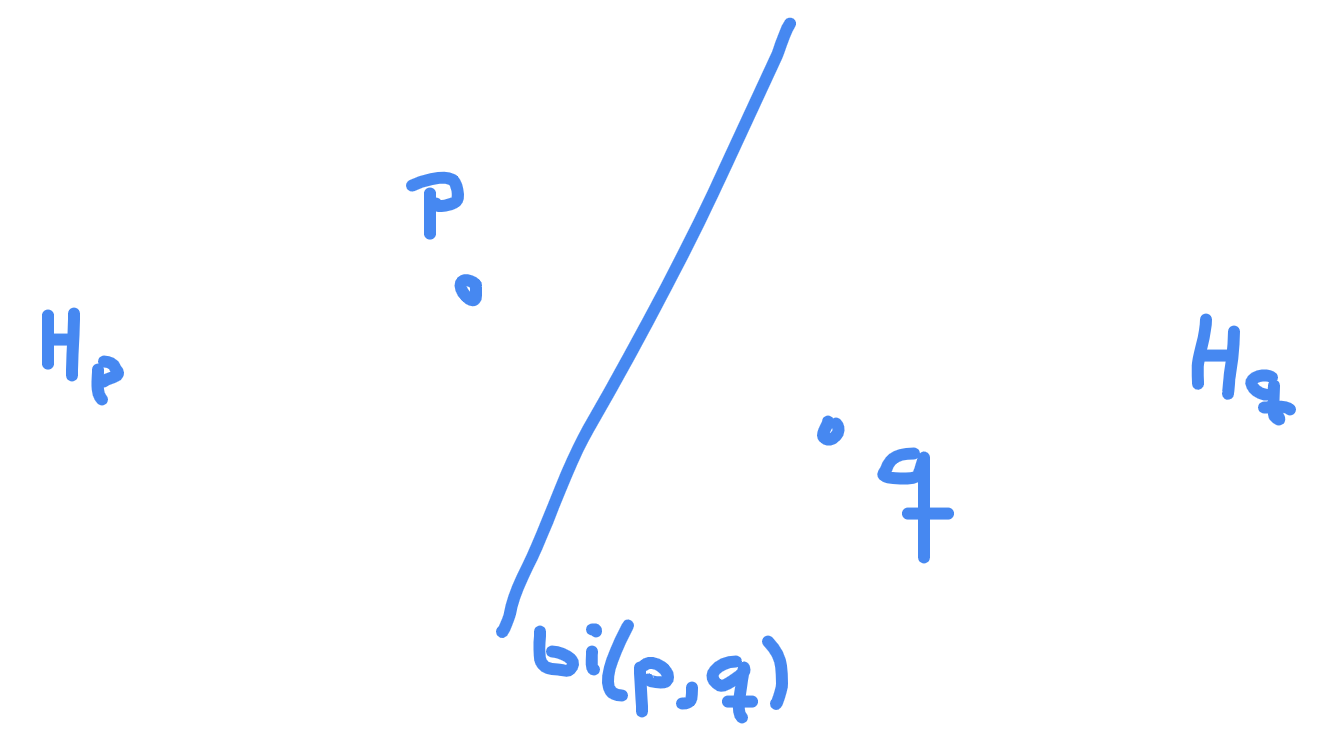
\includegraphics[scale=0.22]{temp-fig-2}
\]
A bisector $\bi(p, q)$ splits the plane into two \textbf{half-planes} $H_p$ and $H_q$ such that $p \in H_p$ and $q \in H_q$. We define $h(p, q)$ to be the open half-plane which contains $p$, that is the interior of $H_p$. So we have that
\[
    \R^2 = h(p, q) \cup \bi(p, q) \cup h(q, p).
\]
\begin{prop} \label{prop:hyperplaneinclusionproperty}
$r \in h(p, q)$ if and only if $\dist(r, p) < \dist(r, q)$.
\end{prop}
\begin{proof}
Let $r \in h(p, q)$ and let $s$ be the projection of $r$ onto the line segment $\overline{pq}$.
\[
    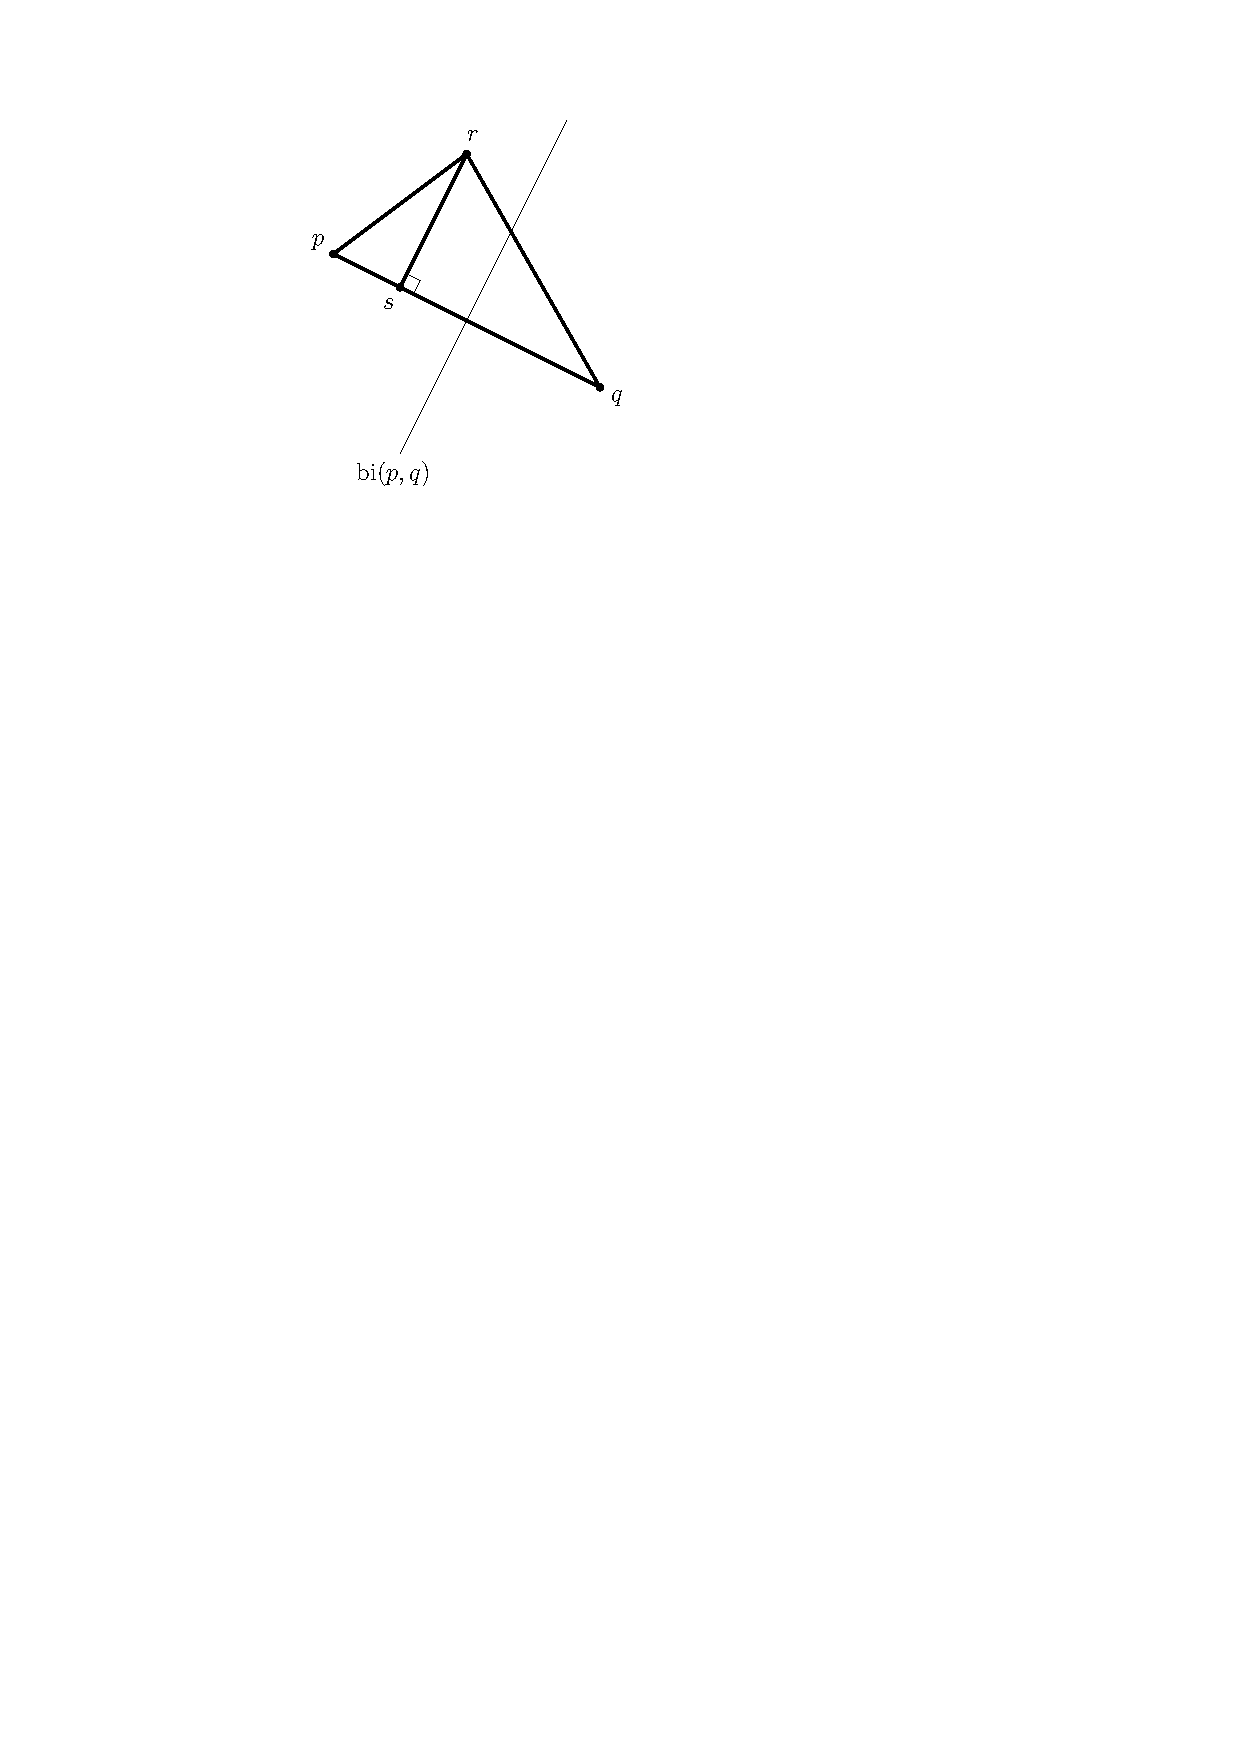
\includegraphics[scale=0.8]{halfplane_containment} %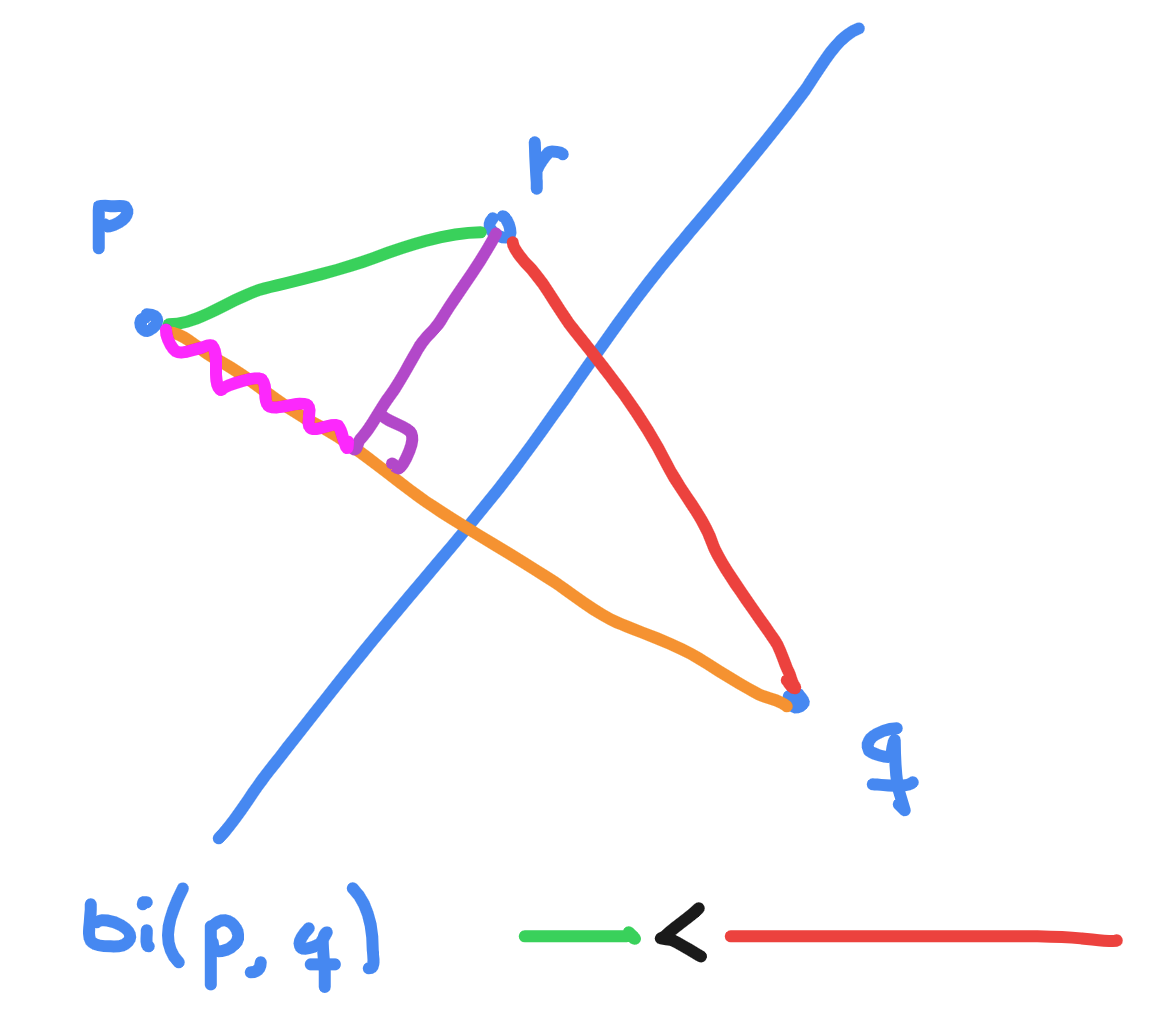
\includegraphics[scale=0.25]{temp-fig-1}
\]
The Pythagorean theorem and the fact that $\overline{ps}$ is shorter than $\overline{sq}$ then gives us
\begin{align*}
    \norm{p - r}^2 &= \norm{p - s}^2 + \norm{s - r}^2 \\
    &< \norm{q - s}^2 + \norm{s - r}^2 \\
    &= \norm{q - r}^2,
\end{align*}
which gives us that $\dist(r, p) < \dist(r, q)$. The other direction is symmetrical.

%\todo{Formalize} Proof sketch: We want to project $r$ onto the orange line. As long as $r \in H_p$ then the squiggly pink segment is shorter than the orange segment, which will make the green segment shorter than the red segment (which is what we want to show).
\end{proof}

\begin{cor} \label{prop:cellsareintersectionsofhalfplanes}
For every Voronoi cell we have
\[
    \mathcal{V}(p_i) = \bigcap_{\substack{1 \leq j \leq n \\ j \ne i}} h(p_i, p_j).
\]
\end{cor}
\begin{proof}
``$\subset$'': Let $r \in \mathcal{V}(p_i)$. Then $\dist(r, p_i) < \dist(r, p_j)$ for all $i \ne j$. Prop \ref{prop:hyperplaneinclusionproperty} then gives us that this is equivalent to $r \in h(p_i, p_j)$ for all $i \ne j$.

``$\supset$'': This argument is symmetrical to the above argument.
\end{proof}
A Voronoi cell is thus the intersection of convex sets and is therefore convex. We conclude that the Voronoi cells are open and convex (possibly unbounded) polygons with at most $n - 1$ vertices and $n - 1$ edges. \\

\section{Shape of the entire diagram}
We now look at the shape of the entire Voronoi diagram. From Corollary \ref{prop:cellsareintersectionsofhalfplanes} it follows that the edges of $\VorG(P)$ are made up of parts of straight lines, namely the bisectors between different points of $P$. We now classify these based on the structure of the points in $P$:
\begin{thm} \label{prop:structureofentirevoronoidiagram}
If the points in $P$ are collinear then $\VorG(P)$ consists of $n - 1$ parallel lines. Otherwise, $\VorG(P)$ is connected and its edges are either segments or half-lines.
\end{thm}
\begin{proof}
Assume that the points in $P$ are collinear. By applying an isometry to $P$, we may assume without loss of generality that the points of $P$ lie on the $x$-axis:
\[
    P = \curly{(x_1, 0), (x_2, 0), \ldots, (x_n, 0)},
\]
where we assume that $x_1 < x_2 < \cdots < x_n$ by rearranging the points if necessary. By definition, we have that $p \in \VorG(P)$ if and only if $p \not\in \mathcal{V}(x_i, 0)$ for all $i$. Let $(x, y) \in \R^2$ such that $x_i < x < x_{i+1}$. Then $(x, y) \in \VorG(P)$ if
\[
    \dist((x, y), (x_i, 0)) = \dist((x, y), (x_{i+1}, 0)).
\]
If furthermore $(x, y) \in \VorG(P)$ then we get
\begin{align*}
    &\norm{(x, y) - (x_i, 0)} = \norm{(x, y) - (x_{i+1}, 0)} \\
    \iff &\sqrt{(x - x_i)^2 + y^2} = \sqrt{(x - x_{i+1})^2 + y^2} \\
    \iff &\abs{x - x_i} = \abs{x - x_{i+1}}.
\end{align*}
Thus if $(x, 0) \in \VorG(P)$ then $(x, y) \in \VorG(P)$ for all $y \in \R$. This shows that $\bi((x_i, 0), (x_{i+1}, 0)) \subset \VorG(P)$ for all $i < n$. Every point of $\VorG(P)$ is on one of these bisectors, and the bisectors are all parallel, which proves the claim.

Assume that the points in $P$ are not collinear. First, we show that the edges of $\VorG(P)$ are either segments or half-lines. Suppose for a contradiction that there is an edge $e$ of $\VorG(P)$ that is a full line and assume that $e \subset \partial\mathcal{V}(p_i) \cap \partial\mathcal{V}(p_j)$. Let $p_k \in P$ be a point which is not collinear with $p_i$ and $p_j$. Then the line $\bi(p_j, p_k)$ is not parallel to the line $e$, hence they have an intersection point. Then there exists a point $v \in e \cap {}^{\circ}h(p_k, p_j)$. The situation is visualized here:
\[
    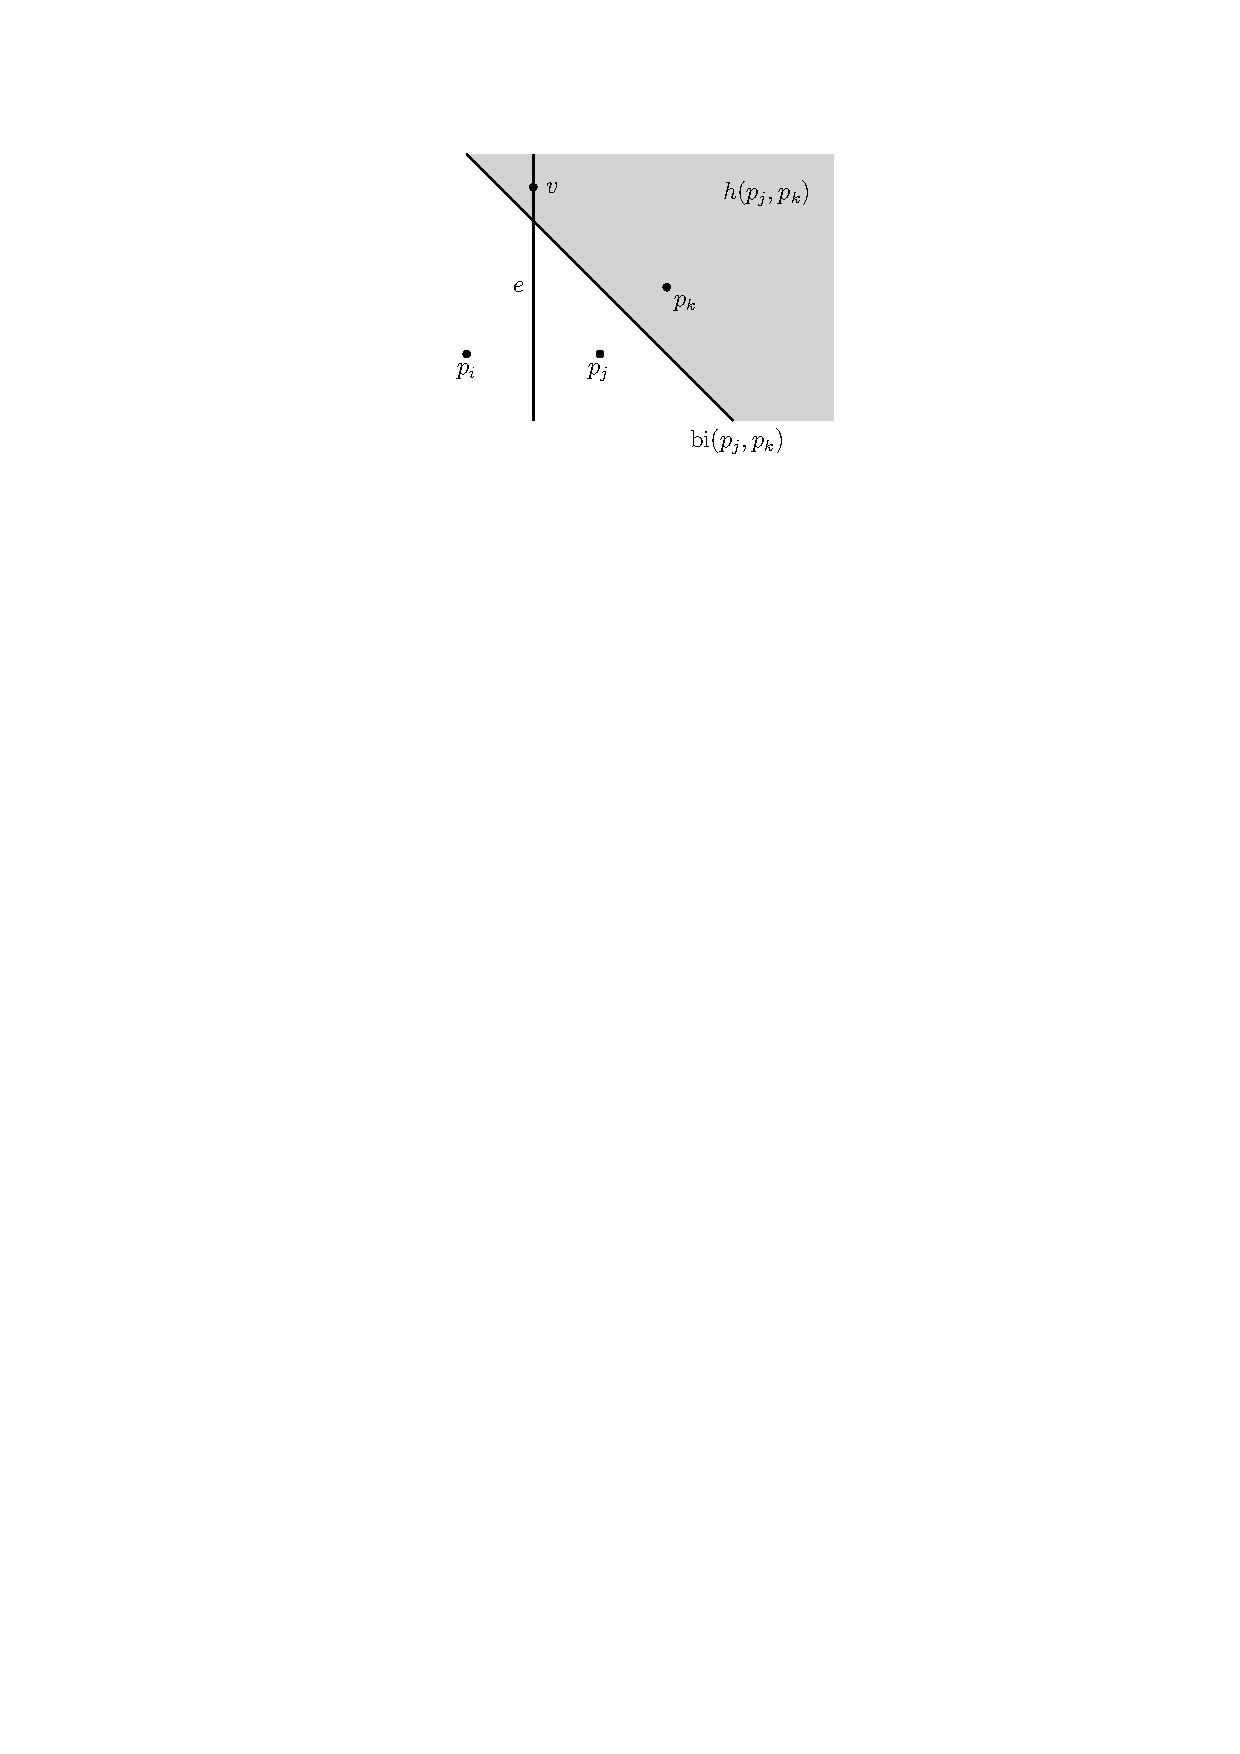
\includegraphics[scale=0.8]{diagram_is_connected} %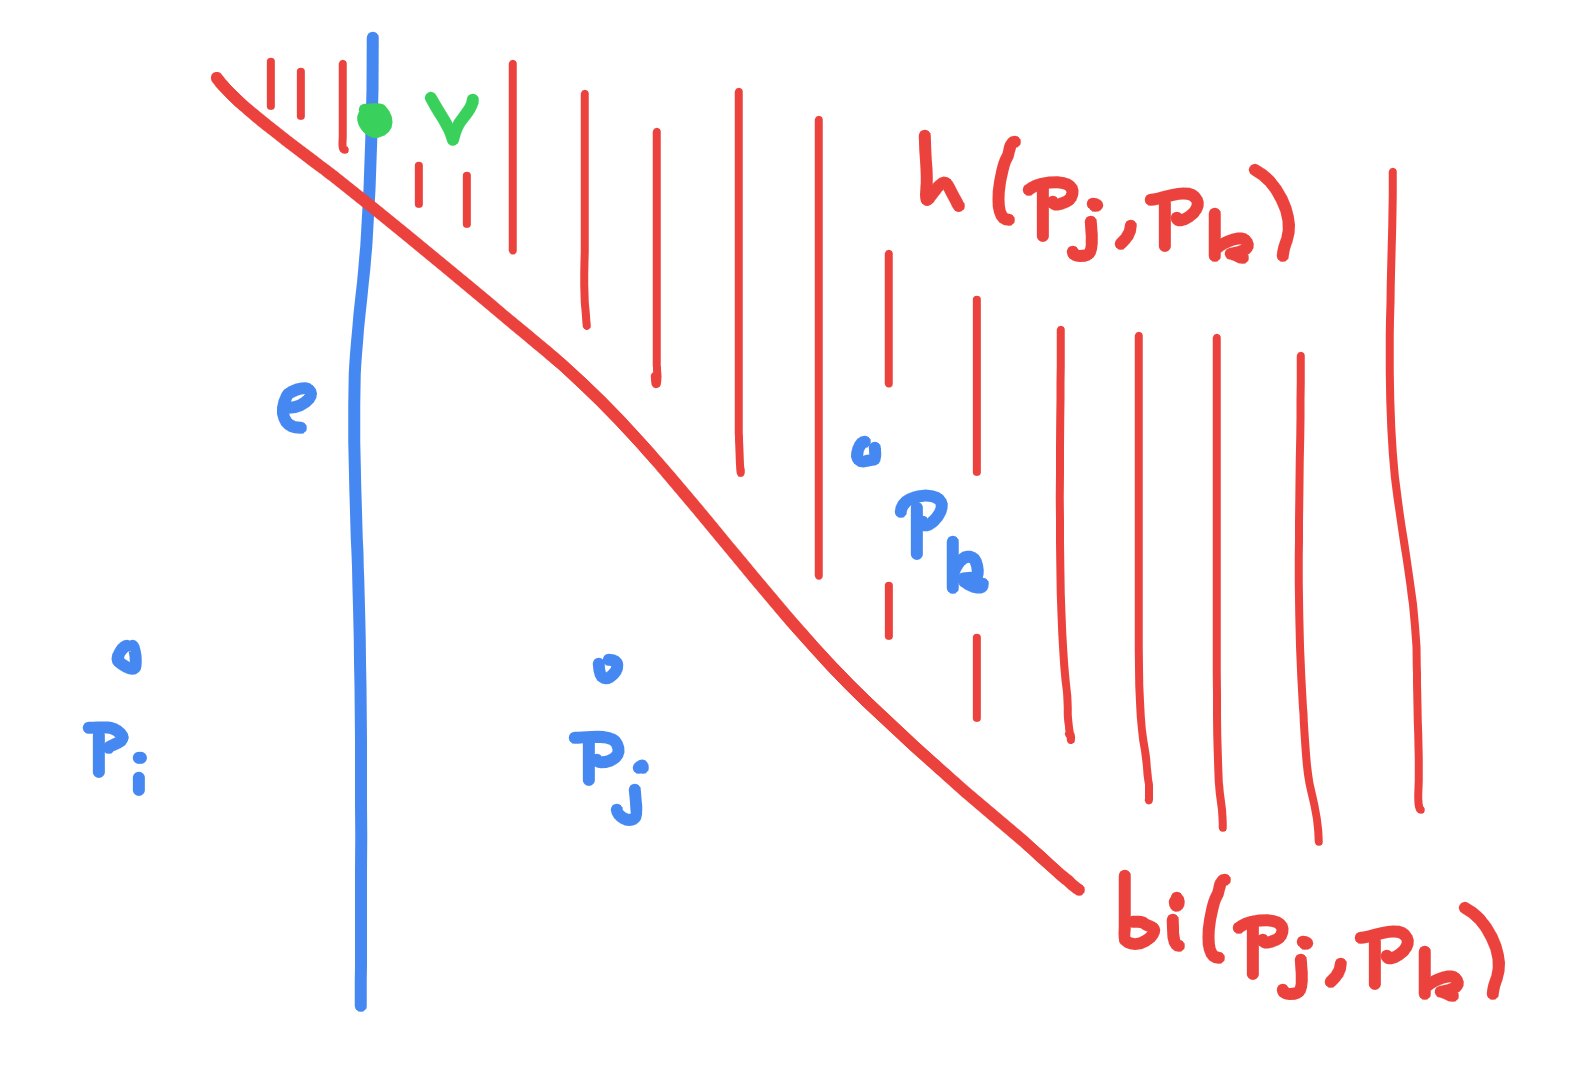
\includegraphics[scale=0.22]{temp-fig-4}
\]
We have that $v \in \partial\mathcal{V}(p_j)$ by definition of $e$. Now note that
\[
    \partial \mathcal{V}(p_j) = \partial \para{\bigcap_{a \ne j} h(p_j, p_a)} \subset^{\footnotemark} \bigcup_{a \ne j} \partial h(p_j, p_a) = \bigcup_{a \ne j} \bi(p_j, p_a).
\]
\footnotetext{Here we used that $\partial(A \cap B) \subset \partial A \cup \partial B$.}As $v \in h(p_k, p_j)$ we have that $\dist(v, p_k) < \dist(v, p_j)$, hence $v \not\in \bi(p_j, p_k)$, so $v \not\in \partial{V}(v_j)$ by the above characterization of $\partial \mathcal{V}(p_j)$.
This is a contradiction, so $e$ can't be a full line. Now we show that $\VorG(P)$ is connected. Assume for the sake of a contradiction that $\VorG(P)$ is not connected. Then there exists a $\partial \mathcal{V}(p_i)$ which is not path connected. This can only happen if $\partial \mathcal{V}(p_i)$ consists of two parallel lines. This contradicts the fact that $\VorG(P)$ contains no lines. Thus $\VorG(P)$ is connected.
\end{proof}

Finally, we show that that the complexity of the vertices and edges is $\mathcal{O}(n)$:
\begin{thm} \label{thm:numberofvertsandedges}
For $n \geq 3$, the number of vertices in $\VorG(P)$ is at most $2n - 5$ and the number of edges is at most $3n - 6$.
\end{thm}
\begin{proof}
If the points in $P$ are collinear, then Theorem \ref{prop:structureofentirevoronoidiagram} implies the claim. Now assume that the points in $P$ are not collinear. As a first preprocessing step, we start by transforming $\VorG(P)$ into an actual plane graph, as some of the edges in $\VorG(P)$ may be half-lines. Let $v_1, \ldots, v_k$ denote the vertices of $\VorG(P)$. Let $p = \tfrac{1}{k}(v_1 + v_2 + \cdots + v_k) \in \R^2$ and let
\[
    r = 1 + \max\curly{\dist(p, v_1), \dist(p, v_2), \ldots, \dist(p, v_k)}.
\]
Then let $B_r(p) \subset \R^2$ denote the open ball with center $p$ and radius $r$. We have that $B_r(p)$ contains every vertex $v_i$ and that every half-line edge $e$ of $\VorG(P)$ intersects $\partial B_r(p)$ exactly once. Now define $v_{\infty} \in \R^2$ as any point in $\R^2 - B_r(p)$ and transform every half-line edge $e$ into a path with finite length by connecting the half-lines to the point $v_{\infty}$. This is possible since $\R^2 - \overline{B_p(r)}$ only contains these half-lines, and every half-line is pointing in a unique direction so we may then transform the half-lines in order by starting with those which are closest to $v_{\infty}$. An example of this construction is given here:
\[
    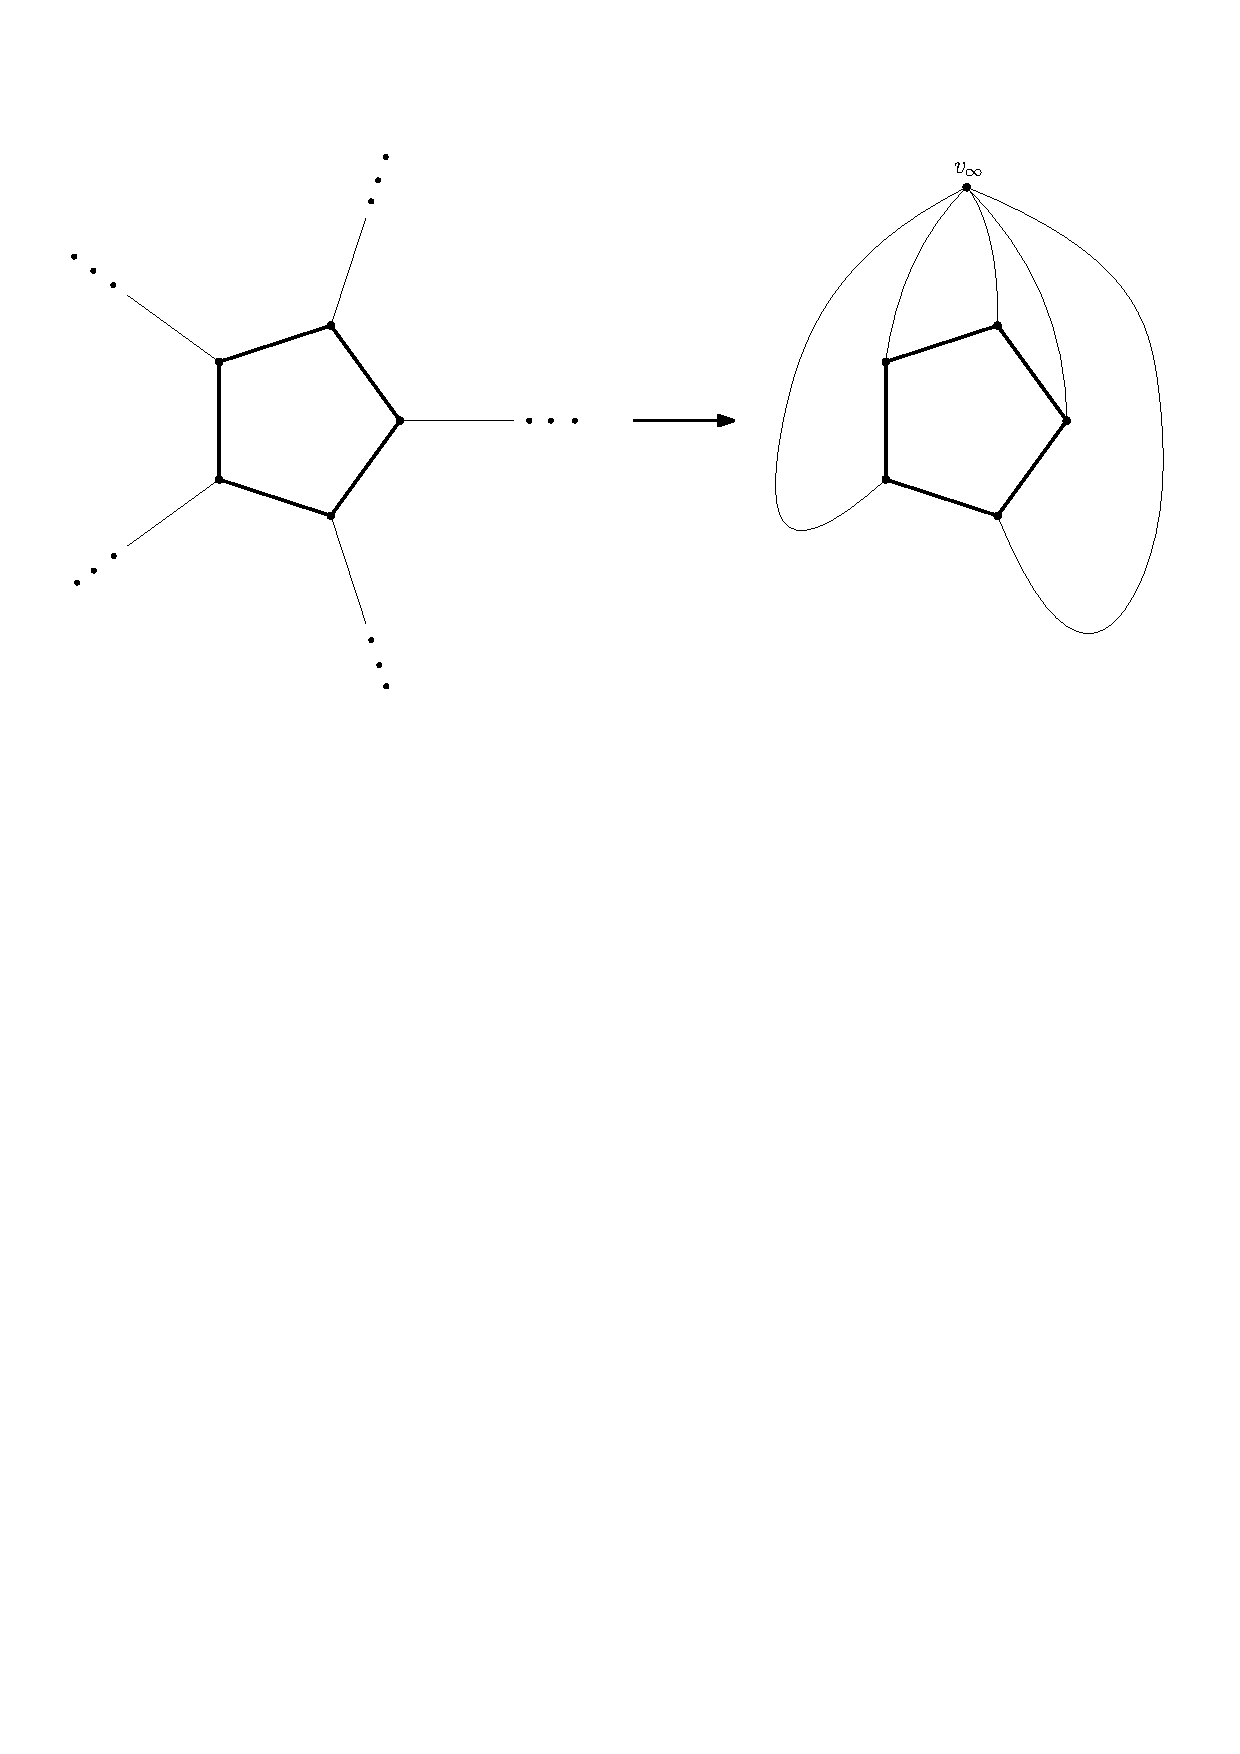
\includegraphics[width=\textwidth]{projective_embedding} % 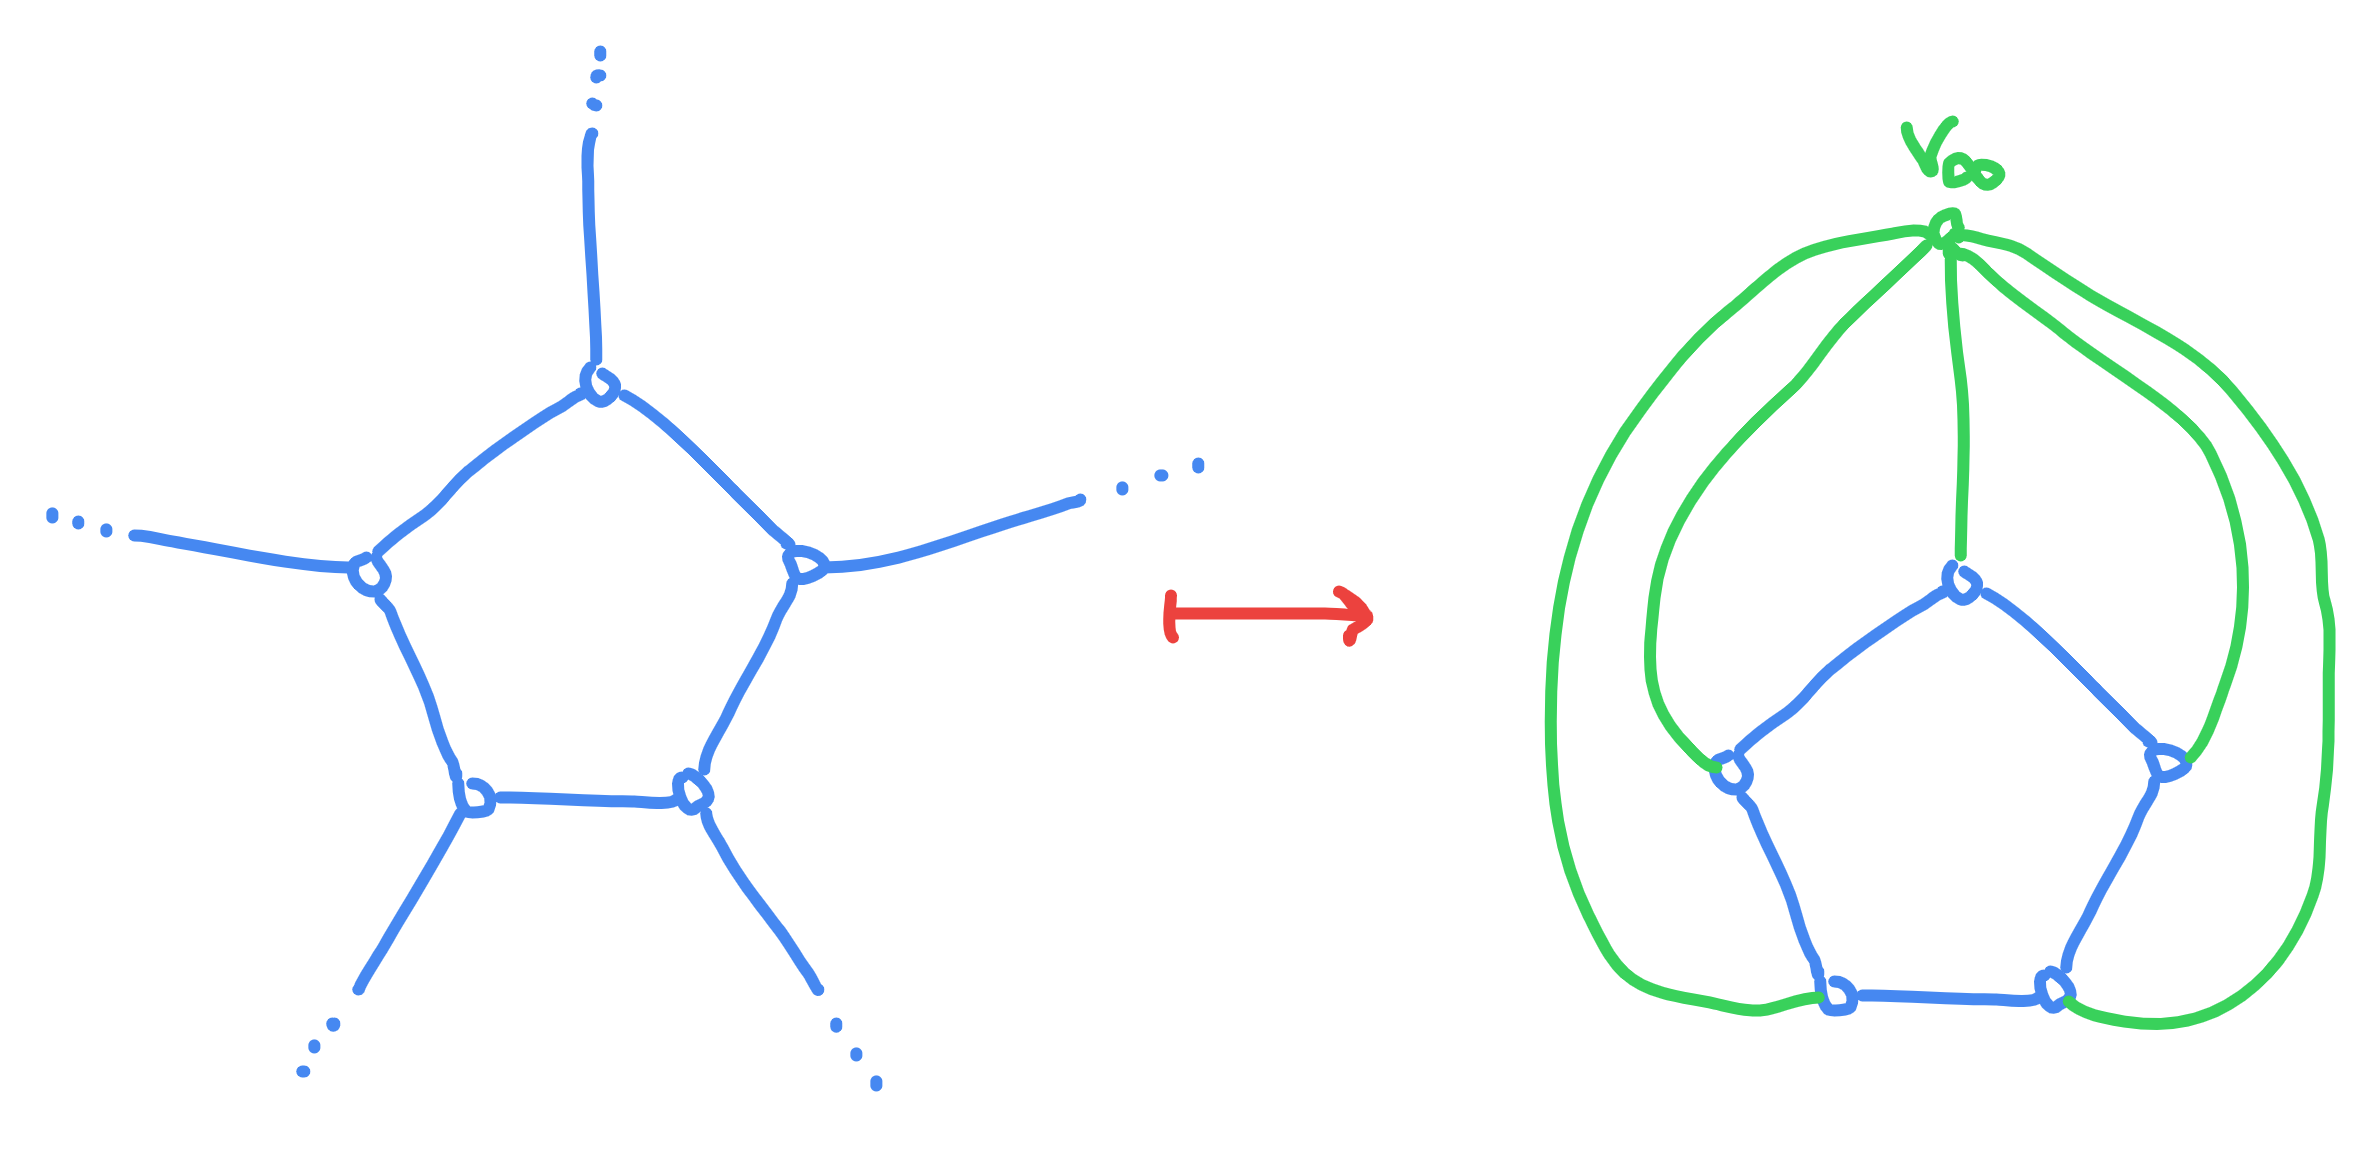
\includegraphics[scale=0.2]{temp-fig-5}
\]
In this way we can turn $\VorG(P)$ into a planar graph. For a planar graph $G$, Euler's polyhedra formula from topology states that
\begin{equation} \label{eq:eulerformulainproof}
    V - E + F = 2,
\end{equation}
where $V$ is the number of vertices, $E$ is the number of edges and $F$ is the number of faces of $G$. Let $n_v$ denote the number of vertices of the original $\VorG(P)$, and let $n_e$ denote the number of edges. In our modification, we only added a single vertex, so by plugging into (\ref{eq:eulerformulainproof}) we obtain the following relationship:
\begin{equation} \label{eq:eulersformulaapplied}
    (n_v + 1) - n_e + n = 2.
\end{equation}
Note that $n$ is the number of faces, since we have a Voronoi cell for each point in $P$. Every vertex $v$ in $G$ has $\deg(v) \geq 3$, otherwise there would be a $\mathcal{V}(p_i)$ which is not convex. This means that
\[
    \sum_{v \in V(G)} \deg(v) \geq 3 \abs{V(G)} = 3(n_v + 1).
\]
Now we want to compute the left side of the above inequality. Given a vertex $v$ we have that $\deg(v)$ counts the number of edges which touch $v$, and in $G$ every edge touches exactly 2 vertices, which gives us that $\sum_{v \in V(G)} \deg(v) = 2 n_e$. Combining these facts, we obtain the inequality:
\begin{equation} \label{ineq:eulersformulacompanion}
    2 n_e \geq 3(n_v + 1).
\end{equation}
Multiplying (\ref{eq:eulersformulaapplied}) by $2$, isolating $2 n_e$ and then applying (\ref{ineq:eulersformulacompanion}) we get:
\begin{align*}
    2 (n_v + 1) - 2 n_e + 2 n = 4
    &\iff 2 n_e = (2 n_v + 1) + 2n - 4 \\
    &\implies 3(n_v + 1) \leq 2 (n_v + 1) + 2n - 4 \\
    &\implies n_v \leq 2n - 5.
\end{align*}
Multiplying (\ref{eq:eulersformulaapplied}) by $3$, isolating $3 (n_v + 1)$ and then applying (\ref{ineq:eulersformulacompanion}) we get:
\begin{align*}
    3 (n_v + 1) - 3 n_e + 3 n = 6
    &\iff 3 (n_v + 1) = 3 n_e - 3n + 6 \\
    &\implies 2 n_e \geq 3n_e - 3n + 6 \\
    &\implies n_e \leq 3n - 6.
\end{align*}
This proves the theorem.
\end{proof}

\section{Characterizing bisectors in the diagram}
We have seen that we have a linear number of vertices and edges $\VorG(P)$, but we have a quadratic number of bisectors $\bi(p_i, p_j)$ of which every edge of $\VorG(P)$ is a subset of, and every vertex in $\VorG(P)$ is an intersection point of two such bisectors. Thus it would be interesting to characterize when a particular bisector is a part of $\VorG(P)$. First, we need a definition:

\begin{defn}[Largest empty circle]
For a $q \in \R^2$ we define $C_P(q)$ to be \emph{the largest empty circle of $q$ with respect to $P$}, which is the largest empty circle with $q$ as its center that does not contain any point of $P$ in its interior. Formally,
\[
    C_P(q) = B_r(q), \quad \text{where} \quad r = \sup\makeset{\lambda \in \R^+}{B_{\lambda}(q) \cap P = \varnothing}.
\]
\end{defn}
\[
    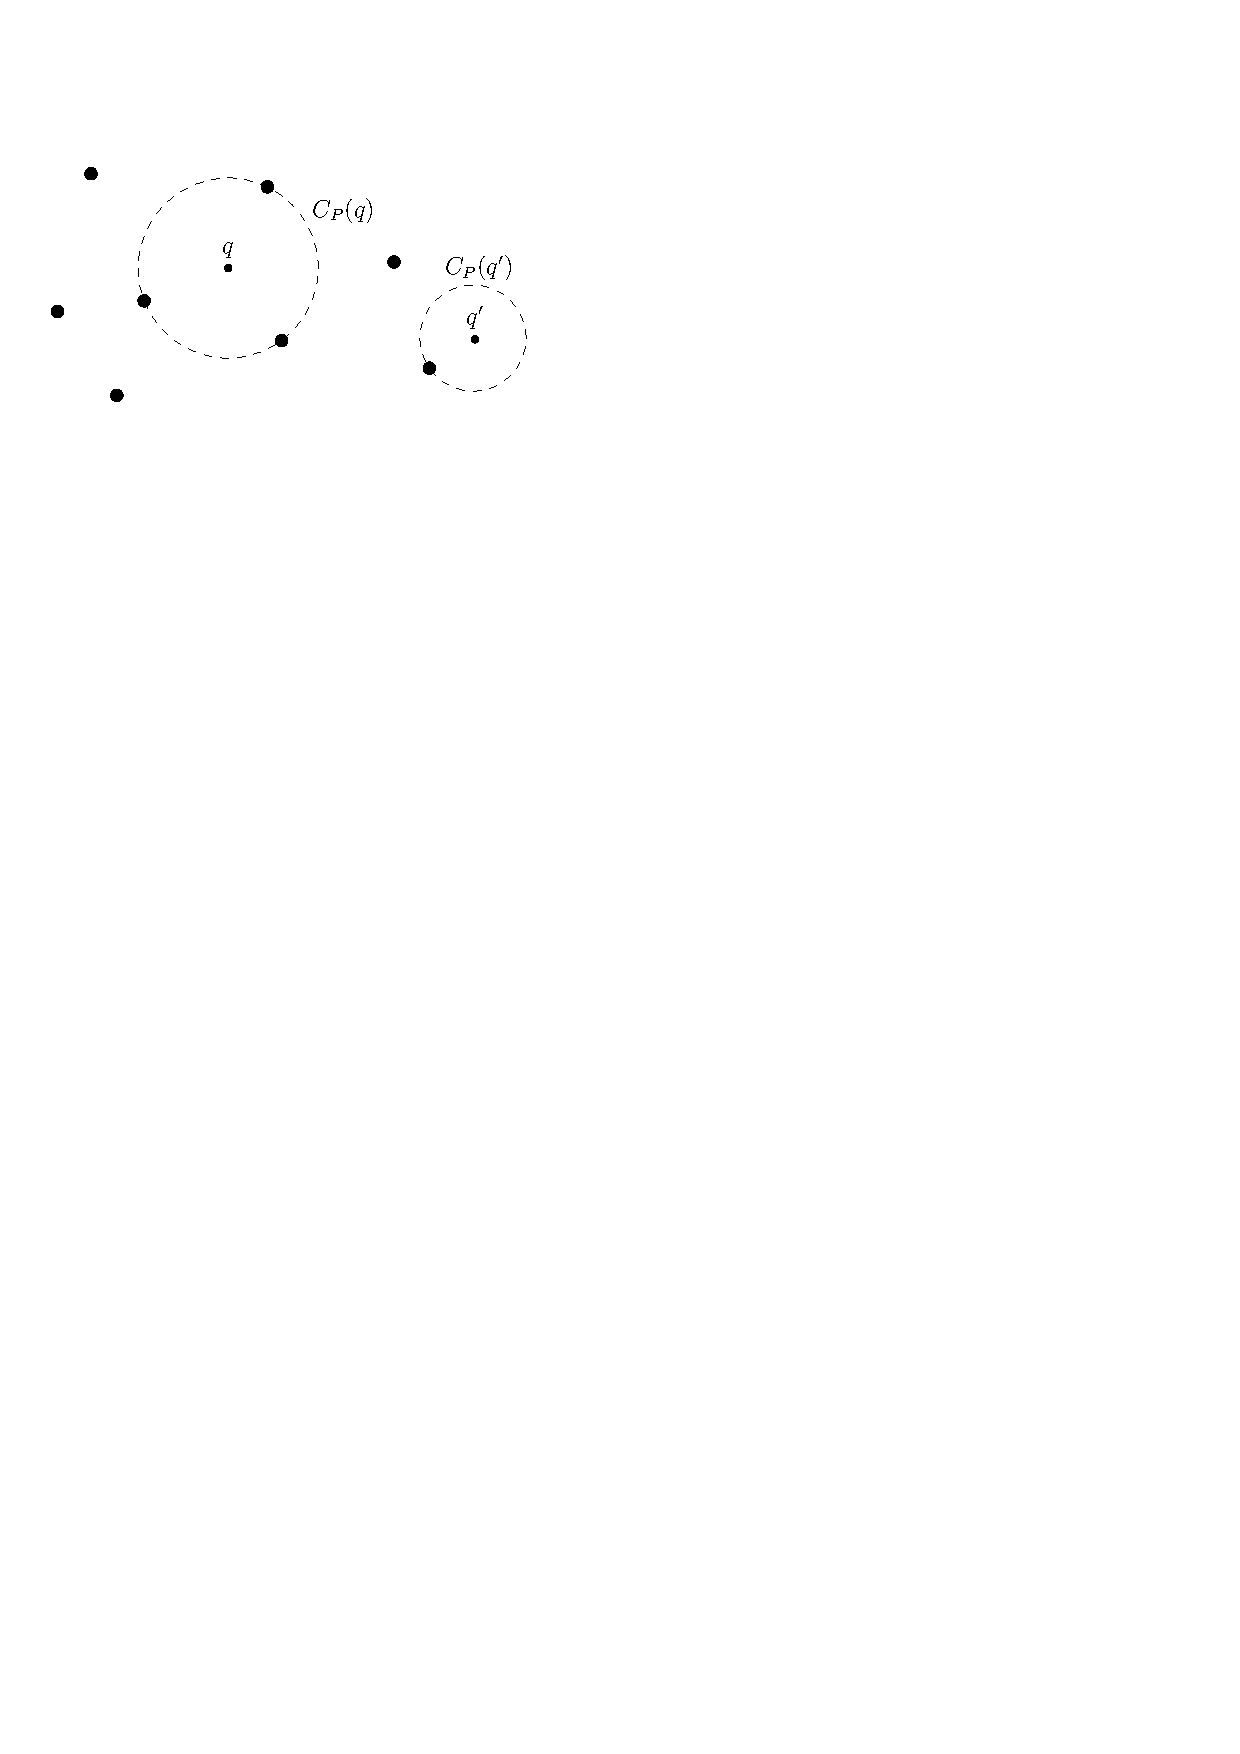
\includegraphics[scale=0.8]{largest_empty_circle}
\]
\begin{thm} \label{thm:characterizationofbisectors} The bisectors and their intersections are characterized by:
\begin{enumerate}[{(}i{)}]
    \item $q \in \R^2$ is a vertex of $\VorG(P)$ if and only if \[ \abs{\partial C_P(q) \cap P} \geq 3. \]
    \item $\bi(p_i, p_j)$ defines an edge of $\VorG(P)$ if and only if \[ \exists q \in \bi(p_i, p_j) \colon \partial C_P(q) \cap P = \curly{p_i, p_j}. \]
\end{enumerate}
\end{thm}
\[
    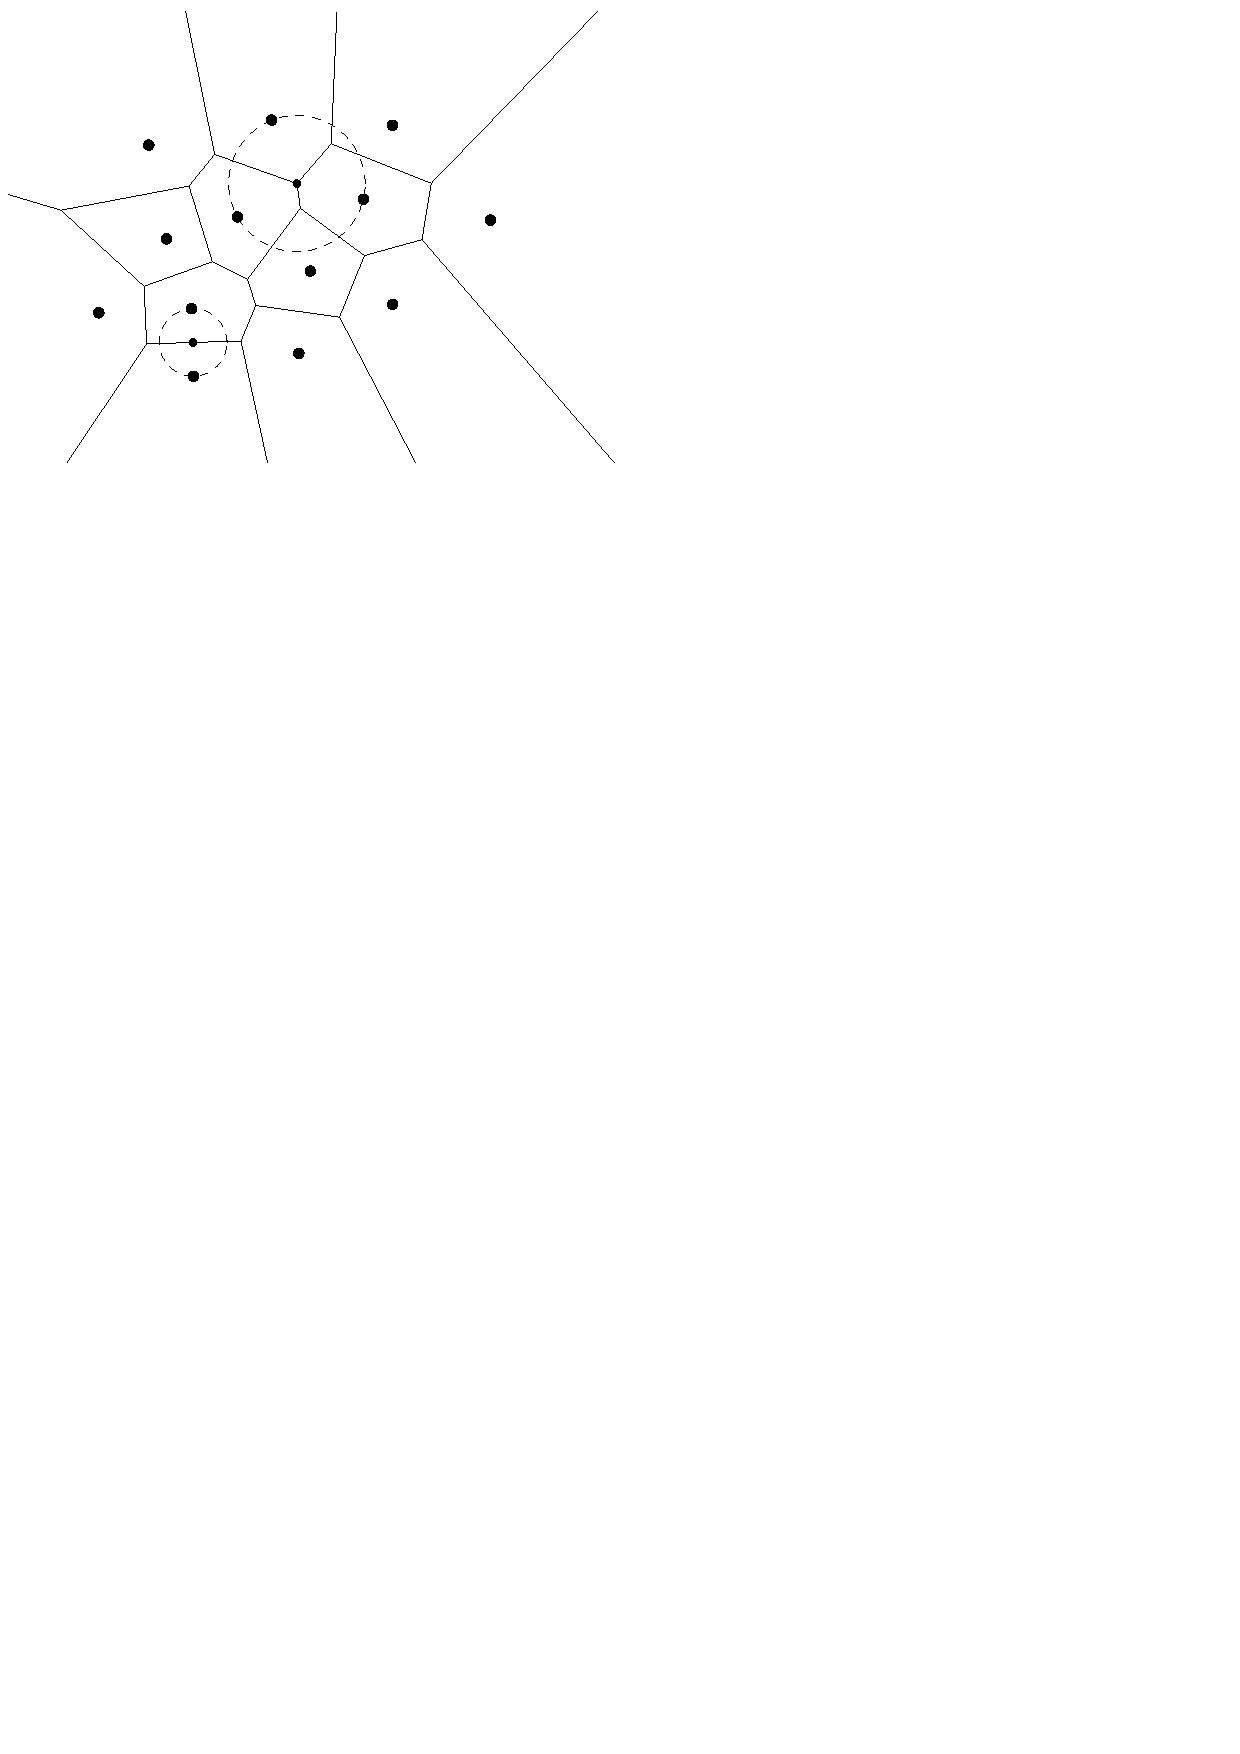
\includegraphics[scale=0.8]{vert_edge_char}
\]
\begin{proof}
We prove each statement individually:
\begin{enumerate}[{(}i{):}]
    \item ``$\Leftarrow$'': Let $q \in \R^2$ and assume that $\abs{\partial C_P(q) \cap P} \geq 3$. Let $p_i, p_j, p_k$ be three distinct points from $\partial C_P(q) \cap P$. Since $C_P(q) \cap P = \varnothing$ by definition, this means that $q$ is equally close to $p_i, p_j, p_k$ but not closer to any other points in $P$, so $q \in \partial\mathcal{V}(p_i) \cap \partial\mathcal{V}(p_j) \cap \partial\mathcal{V}(p_k) \subset \VorG(P)$, and it is a vertex since it is at an intersection of 3 or more bisectors.

    ``$\Rightarrow$'': Let $q \in \R^2$ be a vertex of $\VorG(P)$. A vertex of $\VorG(P)$ touches at least 3 different edges, and thus touches at least 3 distinct Voronoi cells $\mathcal{V}(p_i), \mathcal{V}(p_j)$ and $\mathcal{V}(p_k)$. So $q \in \partial\mathcal{V}(p_i) \cap \partial\mathcal{V}(p_j) \cap \partial\mathcal{V}(p_k)$. This gives us that
    \[
        \dist(q, p_i) = \dist(q, p_j) = \dist(q, p_k).
    \]
    Denote the above distance by $D$. Now assume for the sake of a contradiction that there exists $p_\alpha \in P$ such that $\dist(q, p_{\alpha}) < D$. Then there are parts of the bisectors $\bi(p_{\alpha}, p_i), \bi(p_{\alpha}, p_j), \bi(p_{\alpha}, p_k)$ contained inside $B_D(q)$, which means that $\mathcal{V}(p_i), \mathcal{V}(p_j), \mathcal{V}(p_k)$ do not all meet at $q$, a contradiction. This means that $C_P(q) \cap P = \varnothing$ and $p_i, p_j, p_k \in \partial C_P(q)$.

    \item ``$\Leftarrow$'': Let $q \in \bi(p_i, p_j)$ such that $\partial C_P(q) \cap P = \curly{p_i, p_j}$. So $C_P(q) \cap P = \varnothing$, which by definition of $C_P(q)$ means that
    \[
        \dist(q, p_i) = \dist(q, p_j) \leq \dist(q, p_k)
    \]
    for all $k$. So $q \in \VorG(P)$ and is either a vertex or an edge. Since $\abs{\partial C_P(q) \cap P} < 3$ part (i) gives us that $q$ is not a vertex, hence it must be an edge, which is a subset of $\bi(p_i, p_j)$. 

    ``$\Rightarrow$'': Let $e \subset \bi(p_i, p_j)$ be an edge of $\VorG(P)$. For $q \in e$ we have that $\dist(q, p_i) = \dist(q, p_j)$, and that $q$ touches $\mathcal{V}(p_i)$ and $\mathcal{V}(p_j)$. By applying the same contradiction proof as in (i) ``$\Rightarrow$'' we have that there is no point in $P$ which is closer to $q$ than $p_i$ and $p_j$, thus $\partial C_P(q) \cap P = \curly{p_i, p_j}$.
\end{enumerate}
\end{proof}

% % % % % % % % % % % % % % % % % % % % % % % % % % % % % % % % % % % %
%
% How to store a Voronoi diagram? DCELs
%
% % % % % % % % % % % % % % % % % % % % % % % % % % % % % % % % % % % % 

\section{The DCEL data structure}
We want to write an algorithm to compute the Voronoi diagram, which leads us to a natural question: how do we store Voronoi diagrams on a computer?  We'll need the following geometric data structure:
\begin{defn}[DCEL] \label{defn:dcel}
A \emph{double connected edge list} (DCEL) is a data structure which represents a subdivision of $\R^2$. A DCEL consists of a lists of vertices, faces and edges. For every edge we will have two copies of it, with opposite orientations, so we will refer to each copy as a directed edge and call it a half-edge, so we actually store a list of half-edges. These three structures are represented as follows:
\begin{description}
  \item[\textsf{Vertex}] $v$ -- represents a vertex of the subdivision. Properties:
  \begin{itemize}
    \item $v.\textsf{position} \in \R^2$: Describes the position of $v$.
    \item $v.\textsf{edge} \text{ is a } \textsf{HalfEdge}$: Points to a half-edge which has $v$ as its start vertex.
  \end{itemize}
  \item[\textsf{Face}] $f$ -- represents a face of the subdivision. Properties:
  \begin{itemize}
    \item $f.\textsf{edge} \text{ is a } \textsf{HalfEdge}$: Points to a half-edge which lies on $\partial f$, and which is a part of a cycle of half-edges which goes around $f$ in counterclockwise order.
  \end{itemize}
  \item[\textsf{HalfEdge}] $e$ -- represents a half-edge of the subdivision. Properties:
  \begin{itemize}
    \item $e.\textsf{origin} \text{ is a } \textsf{Vertex}$: Since the half-edge is directed, we have a first and a second vertex in relation to the edge's direction, and this points to the first vertex.
    \item $e.\textsf{twin} \text{ is a } \textsf{HalfEdge}$: Points to the half-edge with the same vertices as $e$, but pointing in the opposite direction.
    \item $e.\textsf{face} \text{ is a } \textsf{Face}$: Points to the face which lies to the left of $e$.
    \item $e.\textsf{next} \text{ is a } \textsf{HalfEdge}$: Around $e.\textsf{face}$ we have a cycle half-edges which is oriented counterclockwise, and given $e$ in this cycle, $e.\textsf{next}$ gives us the next edge.
    \item $e.\textsf{prev} \text{ is a } \textsf{HalfEdge}$: Around $e.\textsf{face}$ we have a cycle half-edges which is oriented counterclockwise, and given $e$ in this cycle, $e.\textsf{prev}$ gives us the previous edge.
  \end{itemize}
\end{description}
\end{defn}

\begin{rmk}
In the CompGeo book the DCEL structure allows a face to have holes, but since Voronoi diagrams and Delaunay triangulations don't have holes in their faces, we have chosen to omit this feature.
\end{rmk}

\begin{ex}
Consider a graph $G$ with 9 vertices and 10 edges embedded into $\R^2$, which is given as the black figure in the following:
\[
    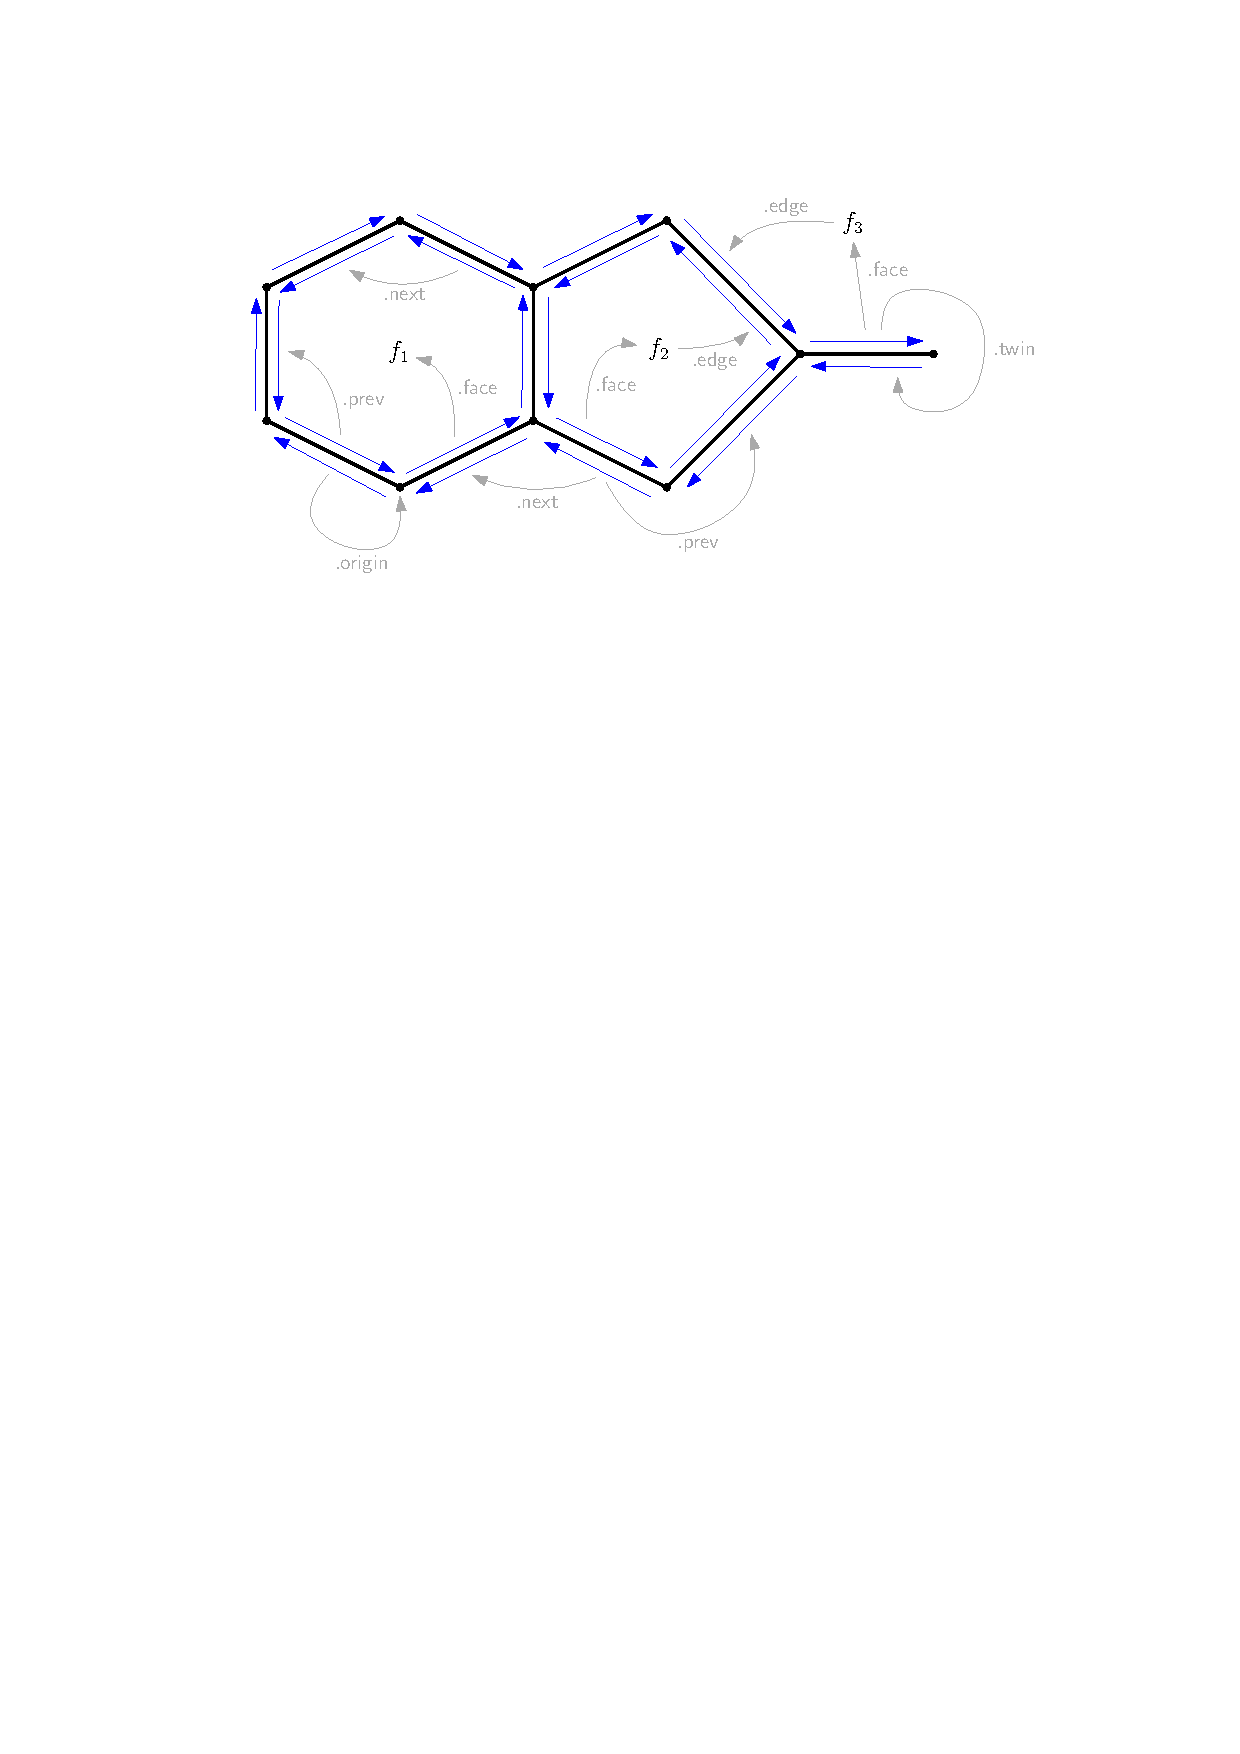
\includegraphics[width=\textwidth]{dcel_example} % 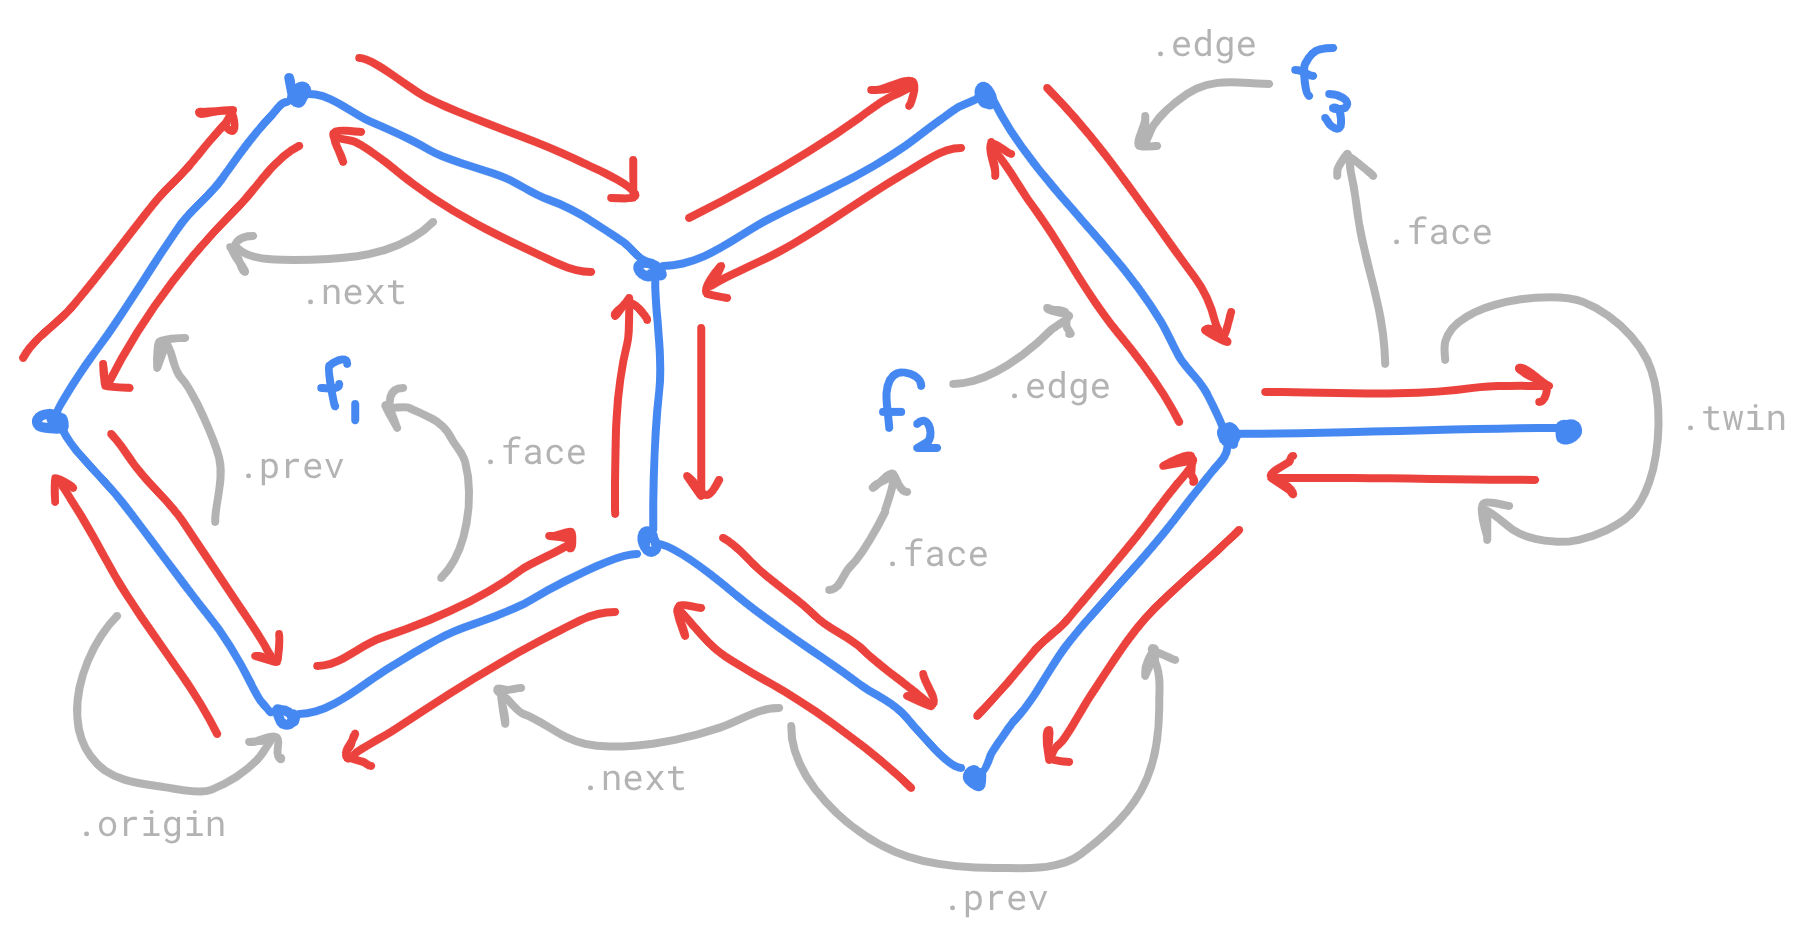
\includegraphics[scale=0.37]{temp-fig-10}
\]
Then this induces a subdivision of $\R^2$ which we represent as a DCEL. The half-edges are given as the blue arrows, the faces as $f_1, f_2, f_3$ and the vertices are the vertices of $G$. Some of the pointers are visible on the figure.
\end{ex}

\begin{rmk} \label{rmk:boxalsohaslinearnumedges}
Note that the DCEL does not support infinite edges, so what we do is put a bounding box $B$ with some padding around the vertices of $\Vor(P)$, and then intersect the infinite edges and faces with the boundary of $B$ and only keep the part inside the bounding box.
\[
    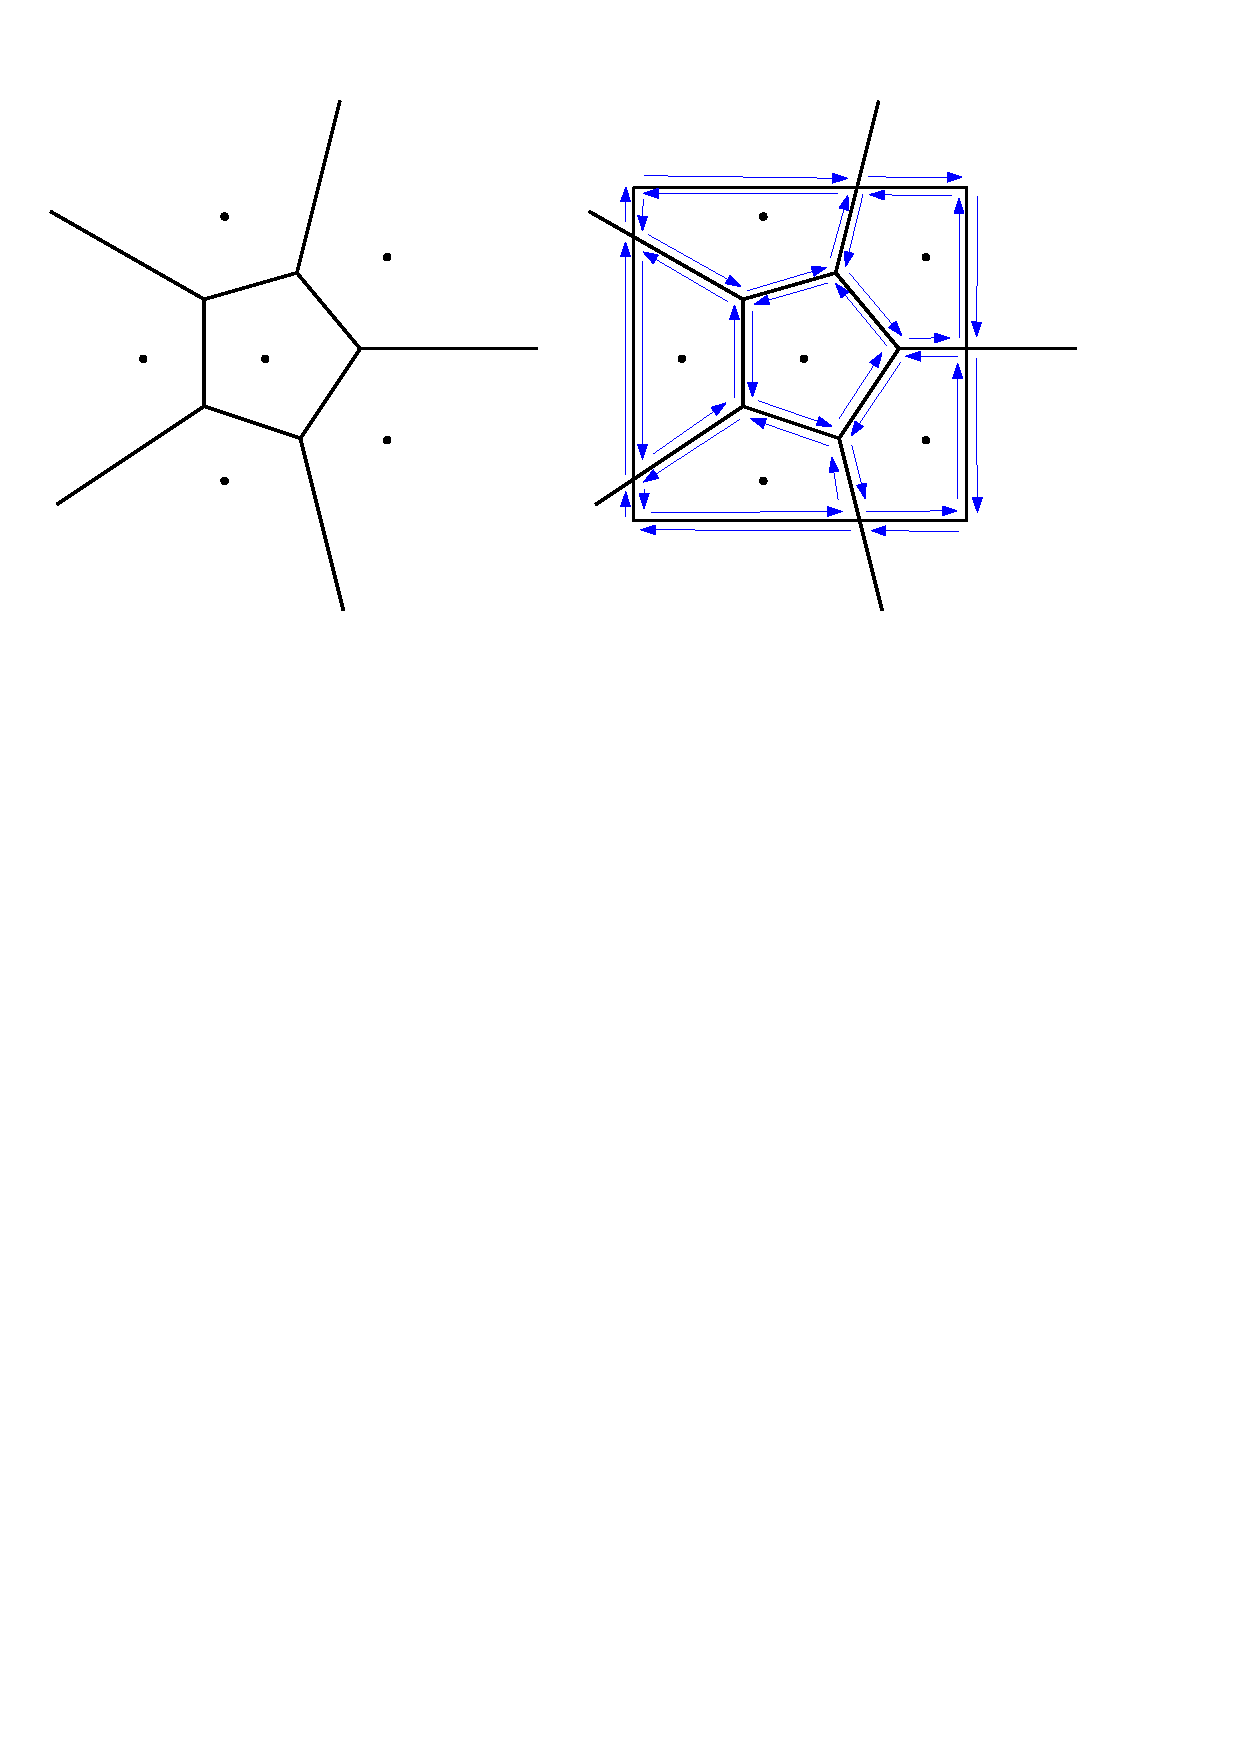
\includegraphics[width=\textwidth]{voronoi_bounding_box} % 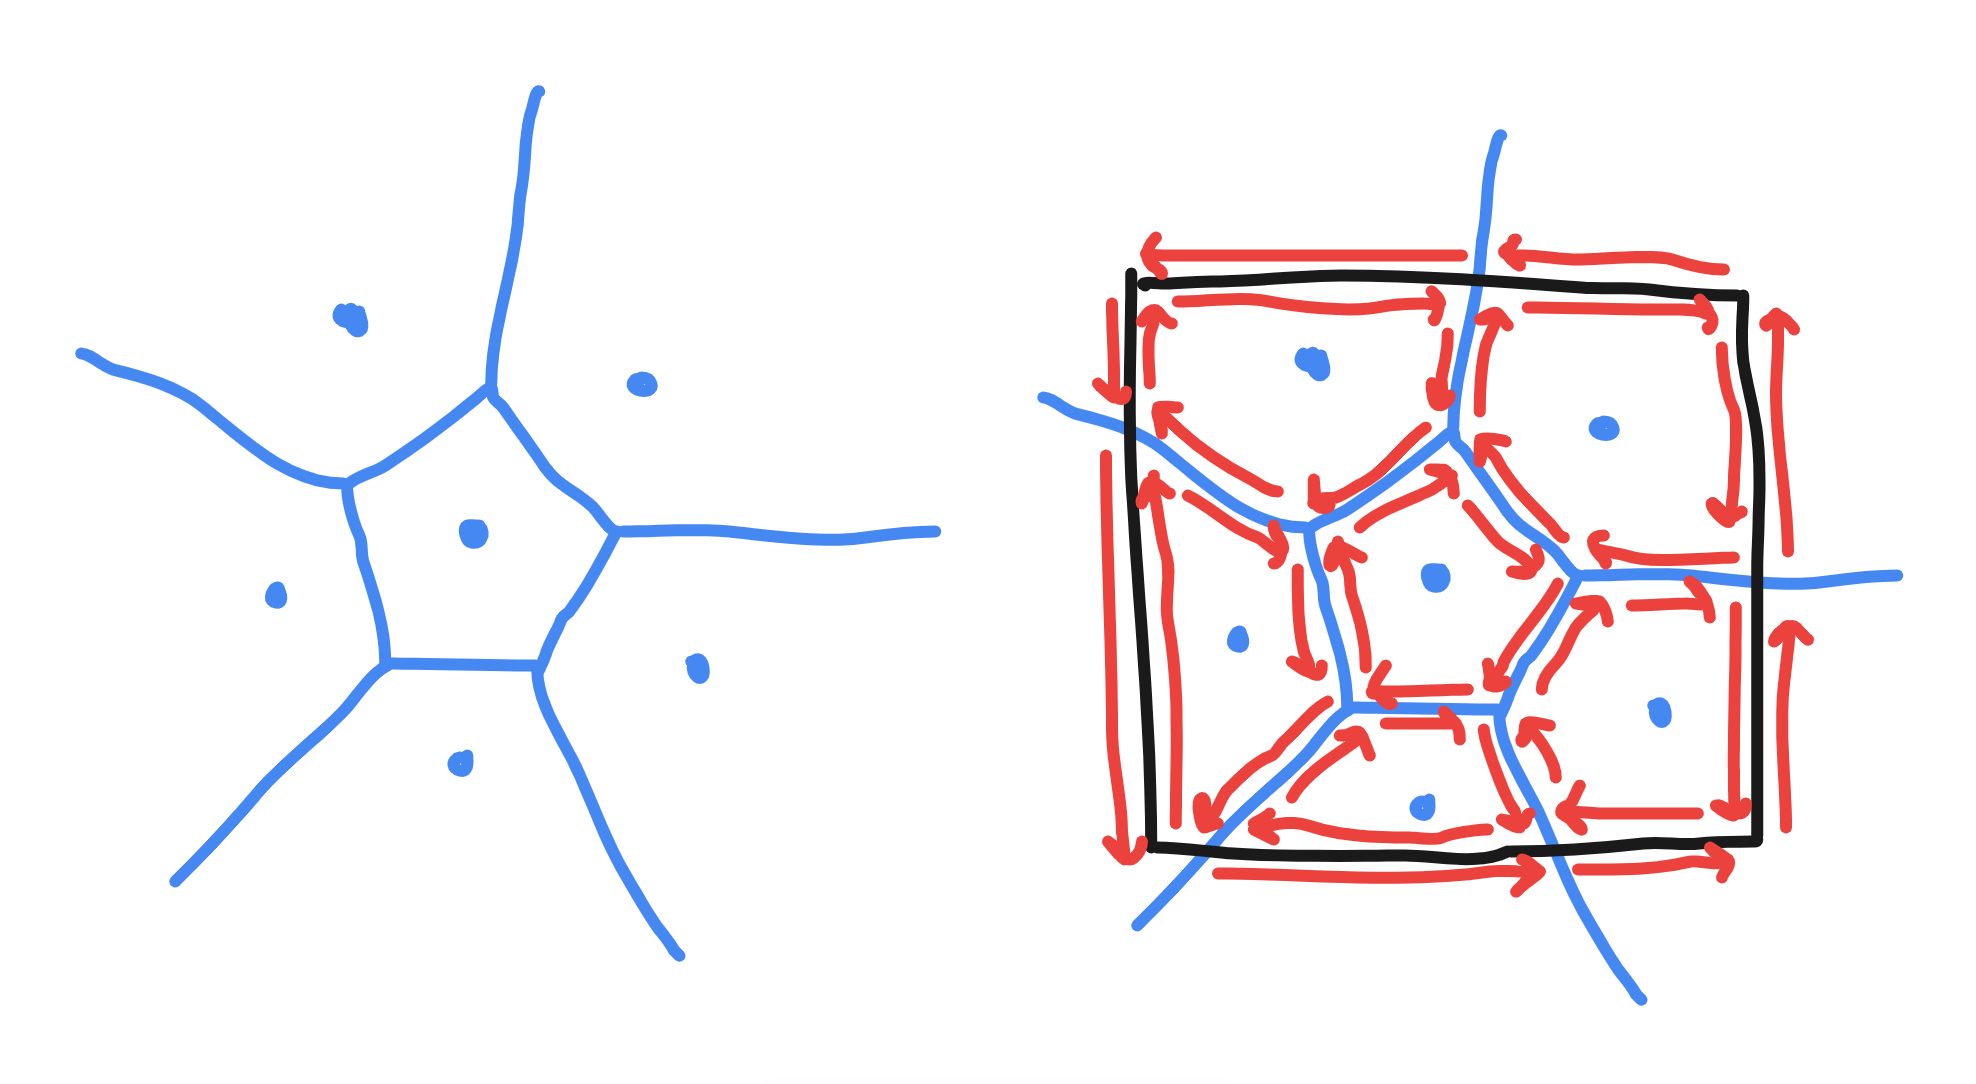
\includegraphics[scale=0.25]{temp-fig-3}
\]
The aim of our algorithms will then be to calculate the DCEL in the right figure.

How does intersecting the edges of $\Vor(P)$ with such a bounding box $B$ affect the number of edges?
\[
    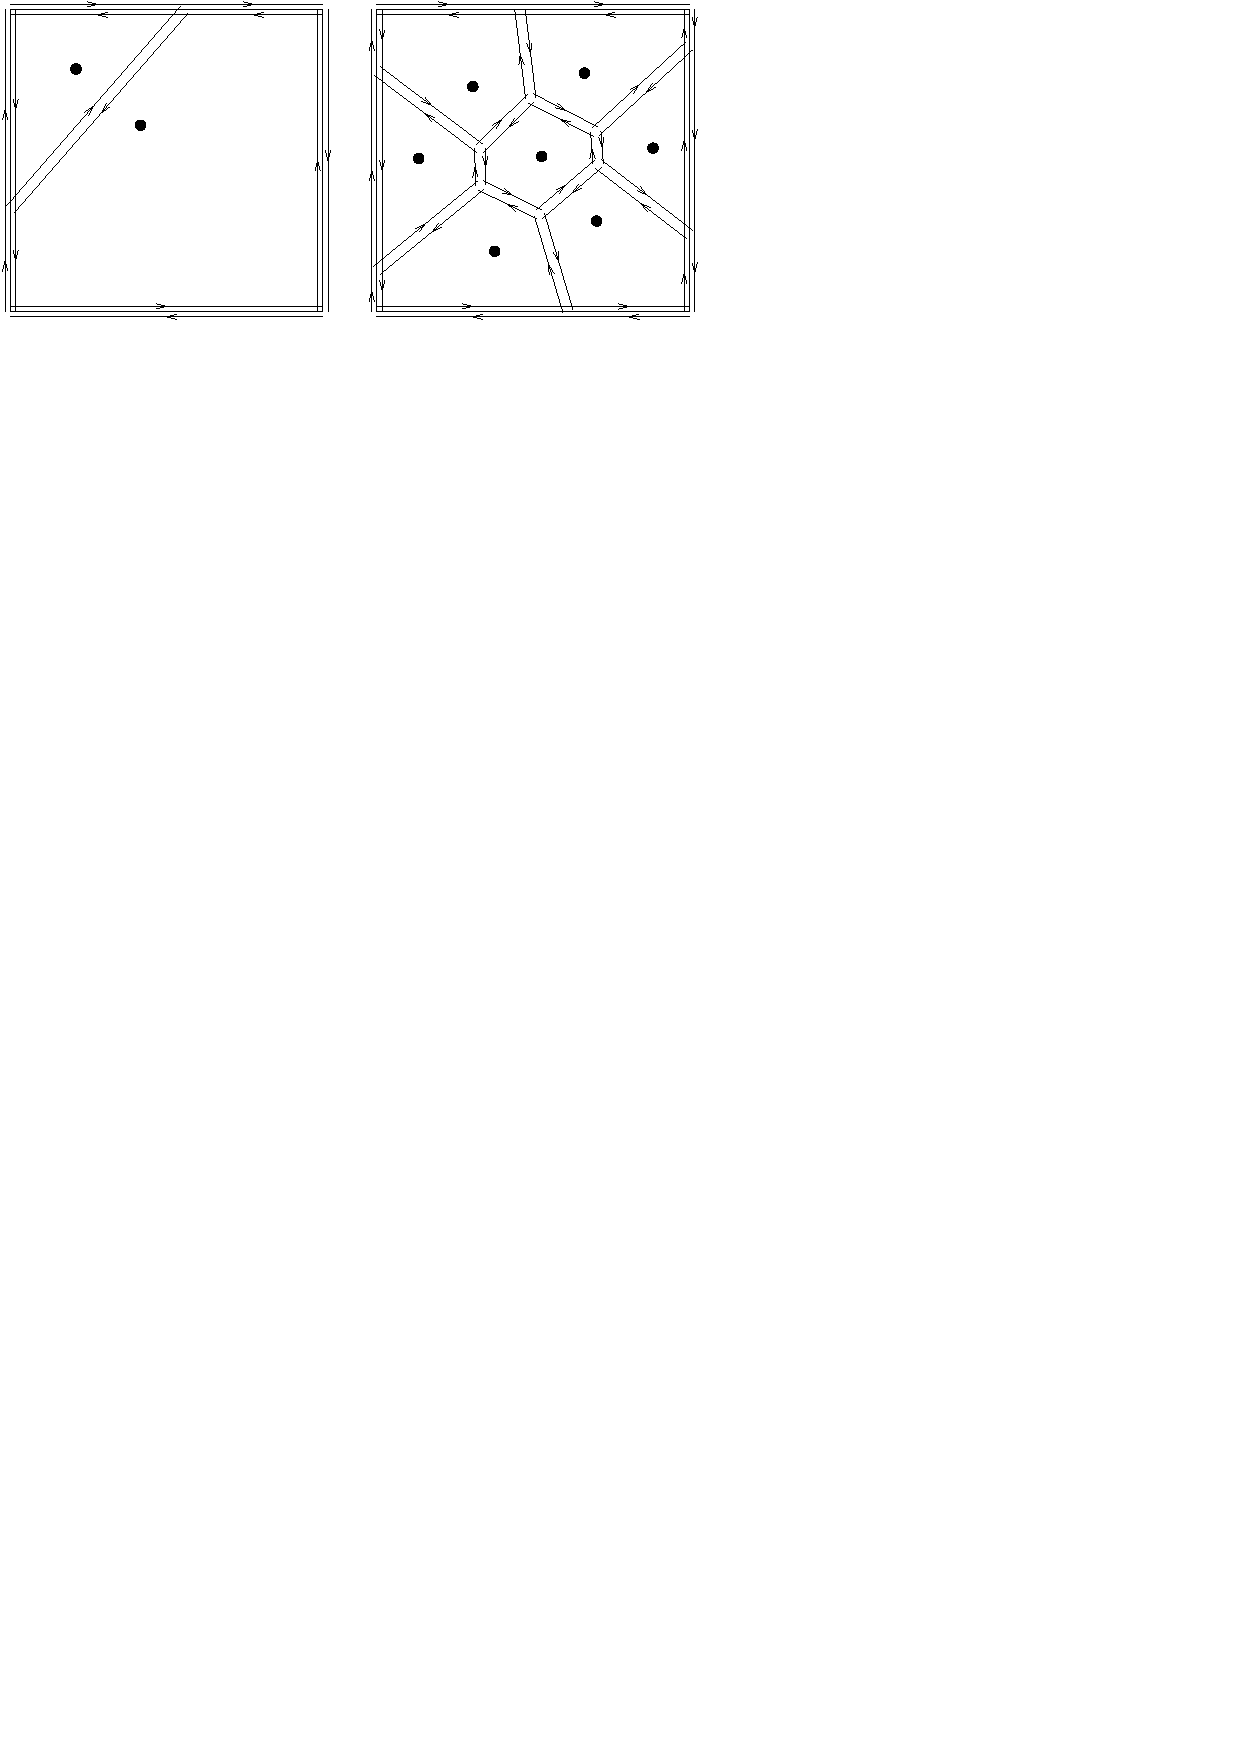
\includegraphics[scale=0.7]{dcel_edges_example}
\]
In the worst case, as depicted on the left figure, 4 new edges may be added to a single unbounded face. In the general case however, as depicted on the right figure, we only introduce between 1-3 edges per face. Thus Theorem \ref{thm:numberofvertsandedges} implies that the complexity is still linear.
%If we intersect $\VorG(P)$ with the bounding box $B$ then $B$ adds at most 2 edges to every cell: The bounded cells inside $B$ stay intact, and for unbounded cells we have two cases. Either a vertex of $B$ is contained in the cell, and then 2 edges will be added, otherwise a single edge is added. Hence in the worst case we add an edge for each point in $P$, and then an edge for each of the 4 corners of $B$, so the DCEL $\Delta$ representing $\Vor(P)$ then has at most
%\[
%    (3n - 6) + (n + 4) = 4n - 2 = \mathcal{O}(n)
%\]
%edges.
\end{rmk}
\chapter{Theory for Fortune's algorithm}

In this chapter we start our treatment on Fortune's algorithm, and it will be our focus for the next three chapters. It is an algorithm for computing the Euclidean Voronoi diagram which has a running time of $\mathcal{O}(n \log n)$. Before we describe the steps of the algorithm, we have to do some theoretical ground work which will help explain why the algorithm works.

\section{Voronoi diagrams can be used to sort}
Before we begin, we show that:

\begin{thm} \label{thm:voronoicansort}
The optimal worst-case running time for computing $\Vor(P)$ is $\mathcal{O}(n \log n)$.
\end{thm}
\begin{proof}
Let $A = \curly{a_1, a_2, \ldots, a_n} \subset \R$ and assume that $n \geq 3$. Define $\varphi \colon \R \to \R^2$ given by $\varphi(x) = (x, x^2)$. Now assume we have used an algorithm to compute a Voronoi diagram of the points
\[
    P = \varphi(A) = \curly{(a_1, a_1^2), (a_2, a_2^2), \ldots, (a_n, a_n^2)}.
\]
We obtain a diagram which looks similar to this:
\[
    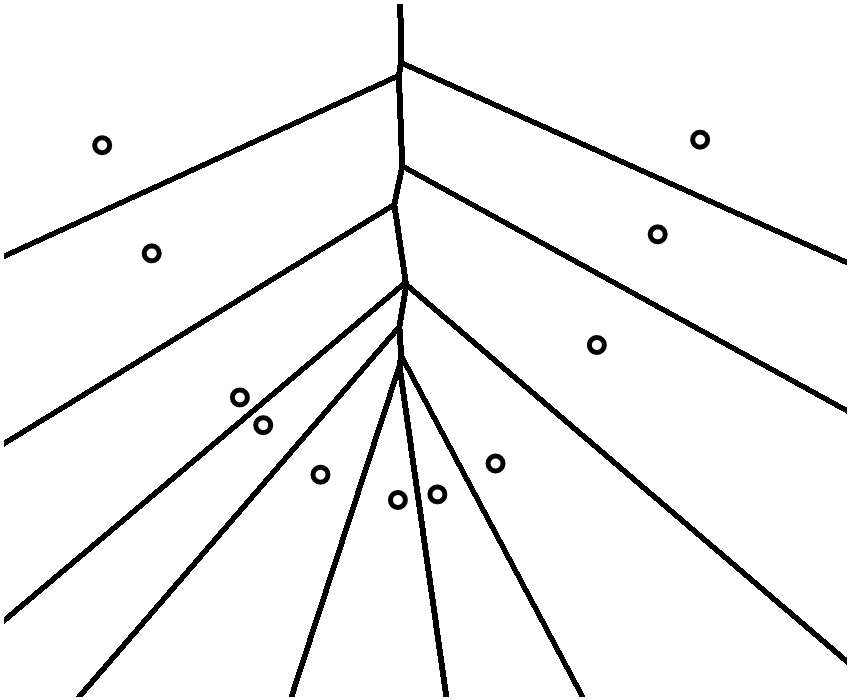
\includegraphics[scale=0.2]{voronoi-sorting-2}
\]
We may assume without loss of generality that $a_i \geq 0$ for all $i$, since we may just add
\[
    \max\makeset{-a}{a \in A \cup \curly{0} \text{ and } a \leq 0}
\]
to every number in $A$. Now we claim that
\begin{equation} \label{goodsortingproperty}
    0 \leq a < b < c < d < e
    \implies
    \begin{cases}
        \dist(\varphi(c), \varphi(b)) < \dist(\varphi(c), \varphi(a)) & \text{ } \\
        \quad\quad\quad\quad\quad\quad \text{ and } \quad & \text{ } \\
        \dist(\varphi(c), \varphi(d)) < \dist(\varphi(c), \varphi(e)). & \text{ }
    \end{cases}
\end{equation}
We have
\[
    \dist(\varphi(x), \varphi(y))^2 = \norm{\varphi(x) - \varphi(y)}^2 = (x - y)^2 + (x^2 - y^2)^2
\]
so
\[
    \dist(\varphi(c), \varphi(b)) < \dist(\varphi(c), \varphi(a))
\]
if and only if
\[
    \underbrace{(c - a)^2 - (c - b)^2}_{\lambda} + \underbrace{(c^2 - a^2)^2 - (c^2 - b^2)^2}_{\mu} > 0.
\]
The fact that $x \mapsto x^2$ is strictly increasing on $[0, \infty)$ and $0 \leq a < b < c$ implies that $\lambda > 0$ and $\mu > 0$. Using a similar argument, we obtain that $\dist(\varphi(c), \varphi(d)) < \dist(\varphi(c), \varphi(e))$. Thus (\ref{goodsortingproperty}) holds.

Now let $B = (b_1, b_2, \ldots, b_n)$ denote $A$ in sorted order, i.e. $i < j$ implies $b_i < b_j$. We'll now see how we can recover $B$ using $\Vor(P)$. We assume that the algorithm outputs a DCEL $\Delta$ of $\Vor(P)$. The property (\ref{goodsortingproperty}) implies that $\partial \mathcal{V}(\varphi(b_i))$ and $\partial \mathcal{V}(\varphi(b_j))$ share an edge when $i = j + 1$. This means that given $\mathcal{V}(\varphi(b_i))$ for $i < n$ we may find $b_{i+1}$ by traversing the edges of $\mathcal{V}(\varphi(b_i))$ in $\Delta$ until we find the face which belongs to $b_{i+1}$. We identify this face as the one which minimizes $a_j - b_i > 0$ where $\mathcal{V}(\varphi(a_j))$ is an adjacent face. In linear time we may find $\ell$ such that $a_{\ell} < a_i$ for all $i \ne \ell$. Let $b_1 := a_{\ell}$. Now assume that $b_i = a_j$ for $i < n$ and some $j$, and that we have the face $F = \mathcal{V}(\varphi(a_j)) \in \Delta$. We traverse the edges of $F$ until we find the face $F' = \mathcal{V}(\varphi(a_k)) \in \Delta$ which belongs to $b_{i+1}$, and we let $b_{i+1} := a_k$. In the worst case we iterate through every edge of every face of $\Delta$, but Remark \ref{rmk:boxalsohaslinearnumedges} gives us that there is $\mathcal{O}(n)$ edges in total, so we find all the $b_i$ in linear time. This means we can use an algorithm which computes $\Vor(P)$ to sort, which proves the claim.
\end{proof}
\todo{Choose a computation model in order for the above to make sense.}

This means that the promised running time of Fortune's algorithm is optimal.

\section{Theoretical assumptions}
In order to make proving some theoretical properties easier, and to avoid not every enlightening edge cases, we will start out by making some assumptions:

\begin{assume} \label{ass:generalposition}
The points in $P$ are in general position, which we define to mean that no two points in $P$ have the same $x$-coordinate or the same $y$-coordinate.
\end{assume}

\begin{assume} \label{ass:notsameline}
The points in $P$ do not all lie on the same line.
\end{assume}

\begin{assume} \label{ass:notcocircular}
No more than 3 points from $P$ lie on the same circle.
\end{assume}

\begin{rmk}
We may make Assumption \ref{ass:generalposition} without loss of generality, because if $\Theta \subset \R$ is the set of all of the angles that $\overline{p_i p_j}$ make with the $x$-axis for all $p_i \ne p_j$ in $P$, then $\Theta$ is finite and $\R \setminus \Theta$ is infinite, so generating a random number $\theta \in \R \setminus \Theta$ and letting
\[
    \varphi (x, y) = \begin{pmatrix} \cos \theta & -\sin \theta \\ \sin \theta & \cos \theta \end{pmatrix} \begin{pmatrix} x \\ y \end{pmatrix}
    = (\cos(\theta) x - \sin(\theta) y, \sin(\theta) x + \cos(\theta) y)
\]
be the rotation about the origin with the angle $\theta$, then the set
\[
    \varphi(P) = \makeset{\varphi(p)}{p \in P}
\]
is in general position with probability 1. After having computed the Voronoi diagram for $\varphi(P)$, we may then rotate the diagram by the angle $-\theta$ to obtain $\Vor(P)$.
\end{rmk}

\begin{rmk}
If $P$ is collinear then every point $p \in P$ lies on a line $\ell$. Theorem \ref{prop:structureofentirevoronoidiagram} gives us that $\VorG(P)$ consists of parallel lines and Theorem \ref{thm:characterizationofbisectors} gives us that these parallel lines are the bisectors of pairs of adjacent points on $\ell$. By sorting the points on $P$ along $\ell$ and then marking all the bisectors between adjacent points we then compute the Voronoi diagram of $\VorG(P)$ in $\mathcal{O}(n \log n)$ time. With this out of the way, it is now reasonable to assume Assumption \ref{ass:notsameline}.
\end{rmk}

\section{The beach line}
In Computational Geometry a sweep line algorithm is an algorithm which incrementally computes some geometric structure, by continuously sweeping a line from one end of the plane to the other. Fortune's algorithm is such an algorithm, and it works by maintaining a horizontal sweep line $\ell \colon y = \ell_y$, and $\ell$ sweeps the plane from top to bottom in order to uncover the structure of the Voronoi diagram. In Fortune's algorithm there is also a secondary device, determined from the current position of the sweep line in relation to the points of $P$. It is called the beach line, and we describe it as follows:

For a point $p = (p_x, p_y) \in \R^2$ and a sweep line $\ell \colon y = \ell_y$ the distance between $p$ and $\ell$ is
\[
    \dist(p, \ell) = \abs{p_y - \ell_y}.
\]
Define
\[
    B_i = \makeset{q \in \R^2}{\dist(q, p_i) = \dist(q, \ell)}
\]
for all $i$. If $(p_i)_y > \ell_y$, it turns out we may parametrize $B_i$ by a parabola: Let $p = (p_x, p_y)$ denote $p_i$ and let $q = (x, y) \in B_i$. Since distances are non-negative, instead of looking at the original definition of $B_i$, it is equivalent to look at satisfying $\dist(q, p)^2 = \dist(q, \ell)^2$. We have:
\[
    \dist(q, p)^2 = \dist(q, \ell)^2 \iff (p_x - x)^2 + (p_y - y)^2 = (y - \ell_y)^2.
\]
This can be transformed into the equation
\begin{equation}
    2 (p_y - \ell_y) y = x^2 - 2 p_x x + p_x^2 + p_y^2 - \ell_y^2.
\end{equation}
Since $p_y \ne \ell_y$ by assumption, we obtain the parabola:
\begin{equation} \label{eq:parabola}
    y = \frac{1}{2 (p_y - \ell_y)} (x^2 - 2 p_x x + p_x^2 + p_y^2 - \ell_y^2),
\end{equation}
which parametrizes $B_i$ if $(p_i)_y > \ell_y$. Now we look at the situation where $(p_i)_y = \ell_y$. Then
\[
    \dist(q, p)^2 = \dist(q, \ell)^2 \iff (p_x - x)^2 + (p_y - y)^2 = (p_y - y)^2.
\]
Then it must be the case that $p_x = x$, so $B_i$ is a subset of a vertical line, and is a line segment if there is some $B_k$ above $B_i$ and a half-line which starts at $p_i$ otherwise. Finally, if $(p_i)_y < \ell_y$, we let $B_i = \varnothing$. We now for all $i$ define the maps
\[
    \beta_i(x) = \begin{cases}
        \displaystyle \frac{x^2 - 2 (p_i)_x x + (p_i)_x^2 + (p_i)_y^2 - \ell_y^2}{2 ((p_i)_y - \ell_y)} & \text{if } (p_i)_y > \ell_y, \\
        \infty & \text{otherwise.}
    \end{cases}
\]
Let $\textsf{LB}(x)$ denote the map which takes the minimum of each $\beta_i$, i.e.
\[
    \textsf{LB}(x) = \min\curly{\beta_1(x), \beta_2(x), \ldots, \beta_n(x)}.
\]
\begin{defn}[Beach line]
The \emph{beach line for the points $P$ with regards to the sweep line $\ell$} is given by the following subset of $\R^2$:
\[
    G \cup V,
    %\makeset{(x, \textsf{LB}(x)) \in \R^2}{\textsf{LB}(x) < \infty} \cup \makeset{B_i - \curly{(p_i)_x} \times (\textsf{LB}((p_i)_x), \infty)}{(p_i)_y = \ell_y}.
\]
where $G$ is the graph of $\textsf{LB}$ when it is finite
\[
    G = \makeset{(x, \textsf{LB}(x)) \in \R^2}{\textsf{LB}(x) < \infty},
\]
and $V$ is all the vertical parts not hidden behind other parabolas
\[
    V = \makeset{B_i - \curly{(p_i)_x} \times (\textsf{LB}((p_i)_x), \infty)}{i = 1, \ldots, n \text{ where } (p_i)_y = \ell_y}.
\]
\end{defn}
In the figure below the beach line is illustrated by the blue curves:
\[
    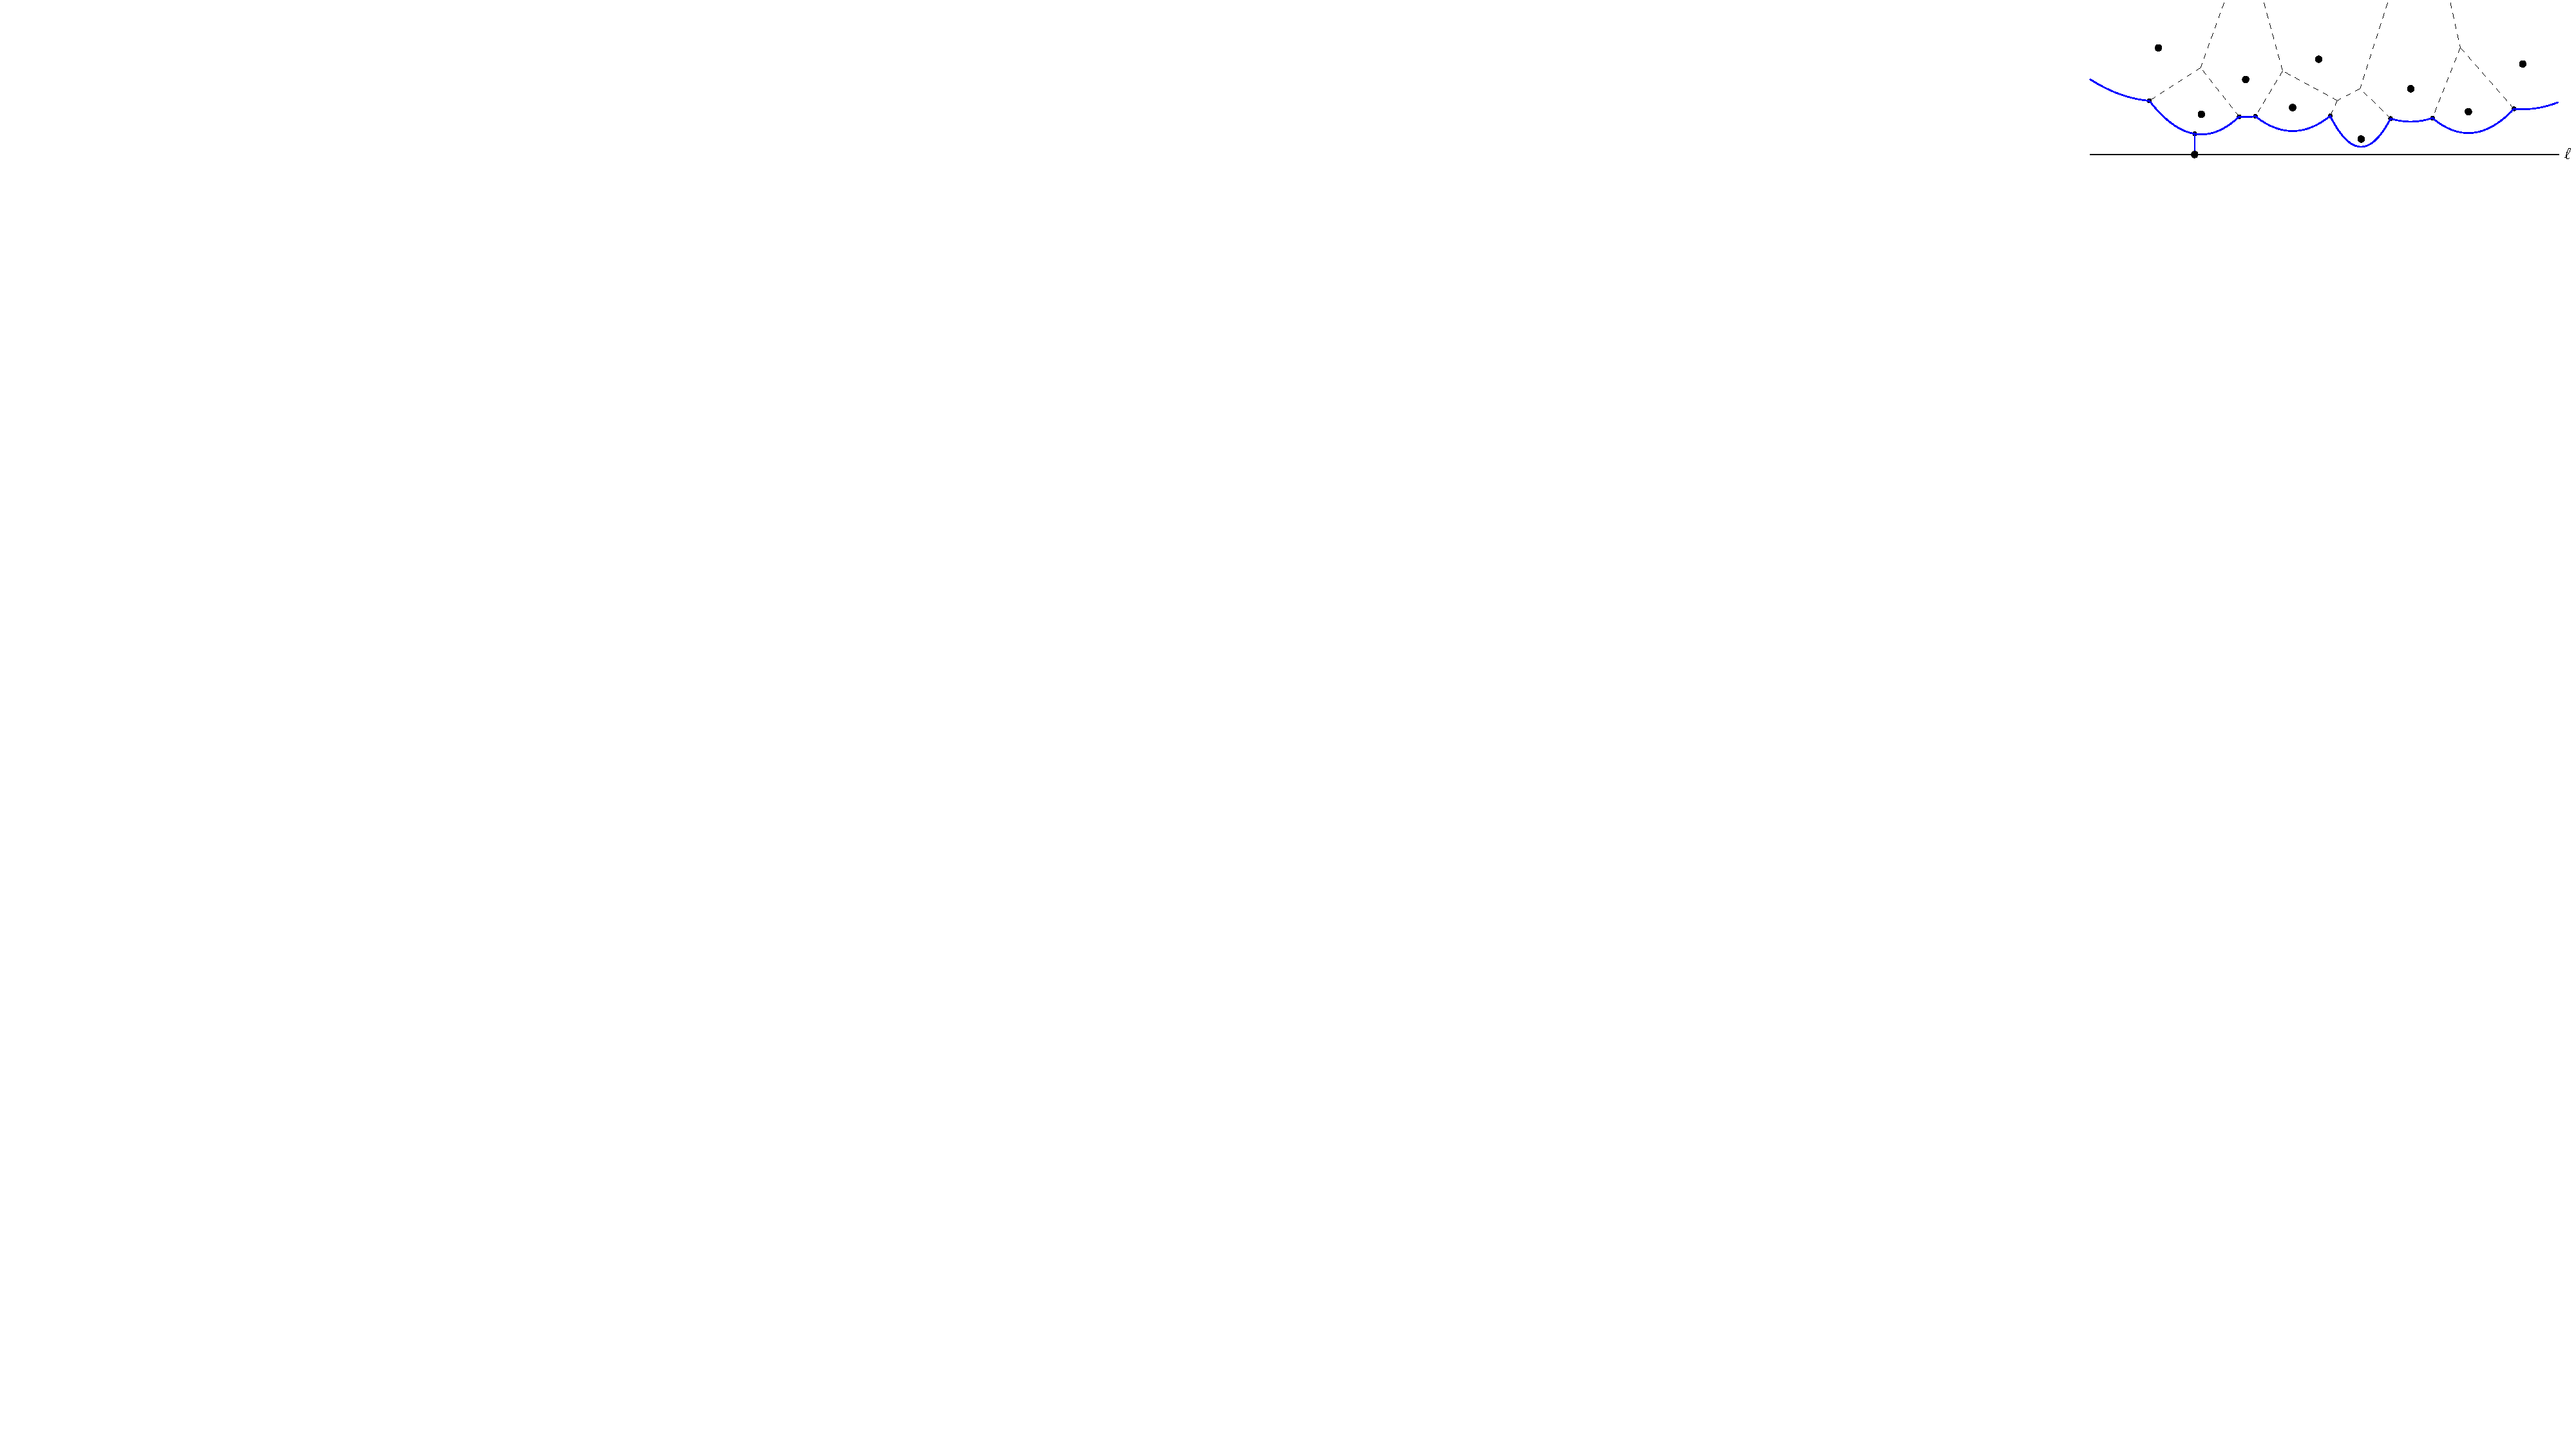
\includegraphics[width=\textwidth]{beachline}
\]
\begin{rmk}
From the definition we see that the beach line consists of parts of parabolas, and vertical line segments or half-lines. For this reason, it is easy to see that the intersection between any vertical line and the beach line has at most one component.
\end{rmk}
\begin{rmk}
For a sweep line $\ell$ which does not intersect any of the points in $P$, it follows from the definition of beach line that the map $\textsf{LB}(x)$ parametrizes the beach line. This was used in the demo to visualize the beach line.
\end{rmk}
\begin{defn}[Breakpoint]
Every point $q$ on the beach line such that $q \in B_i \cap B_j$ for two different $i, j$ is called a \textit{breakpoint}.
\end{defn}

\begin{figure}[H]
    \centering
    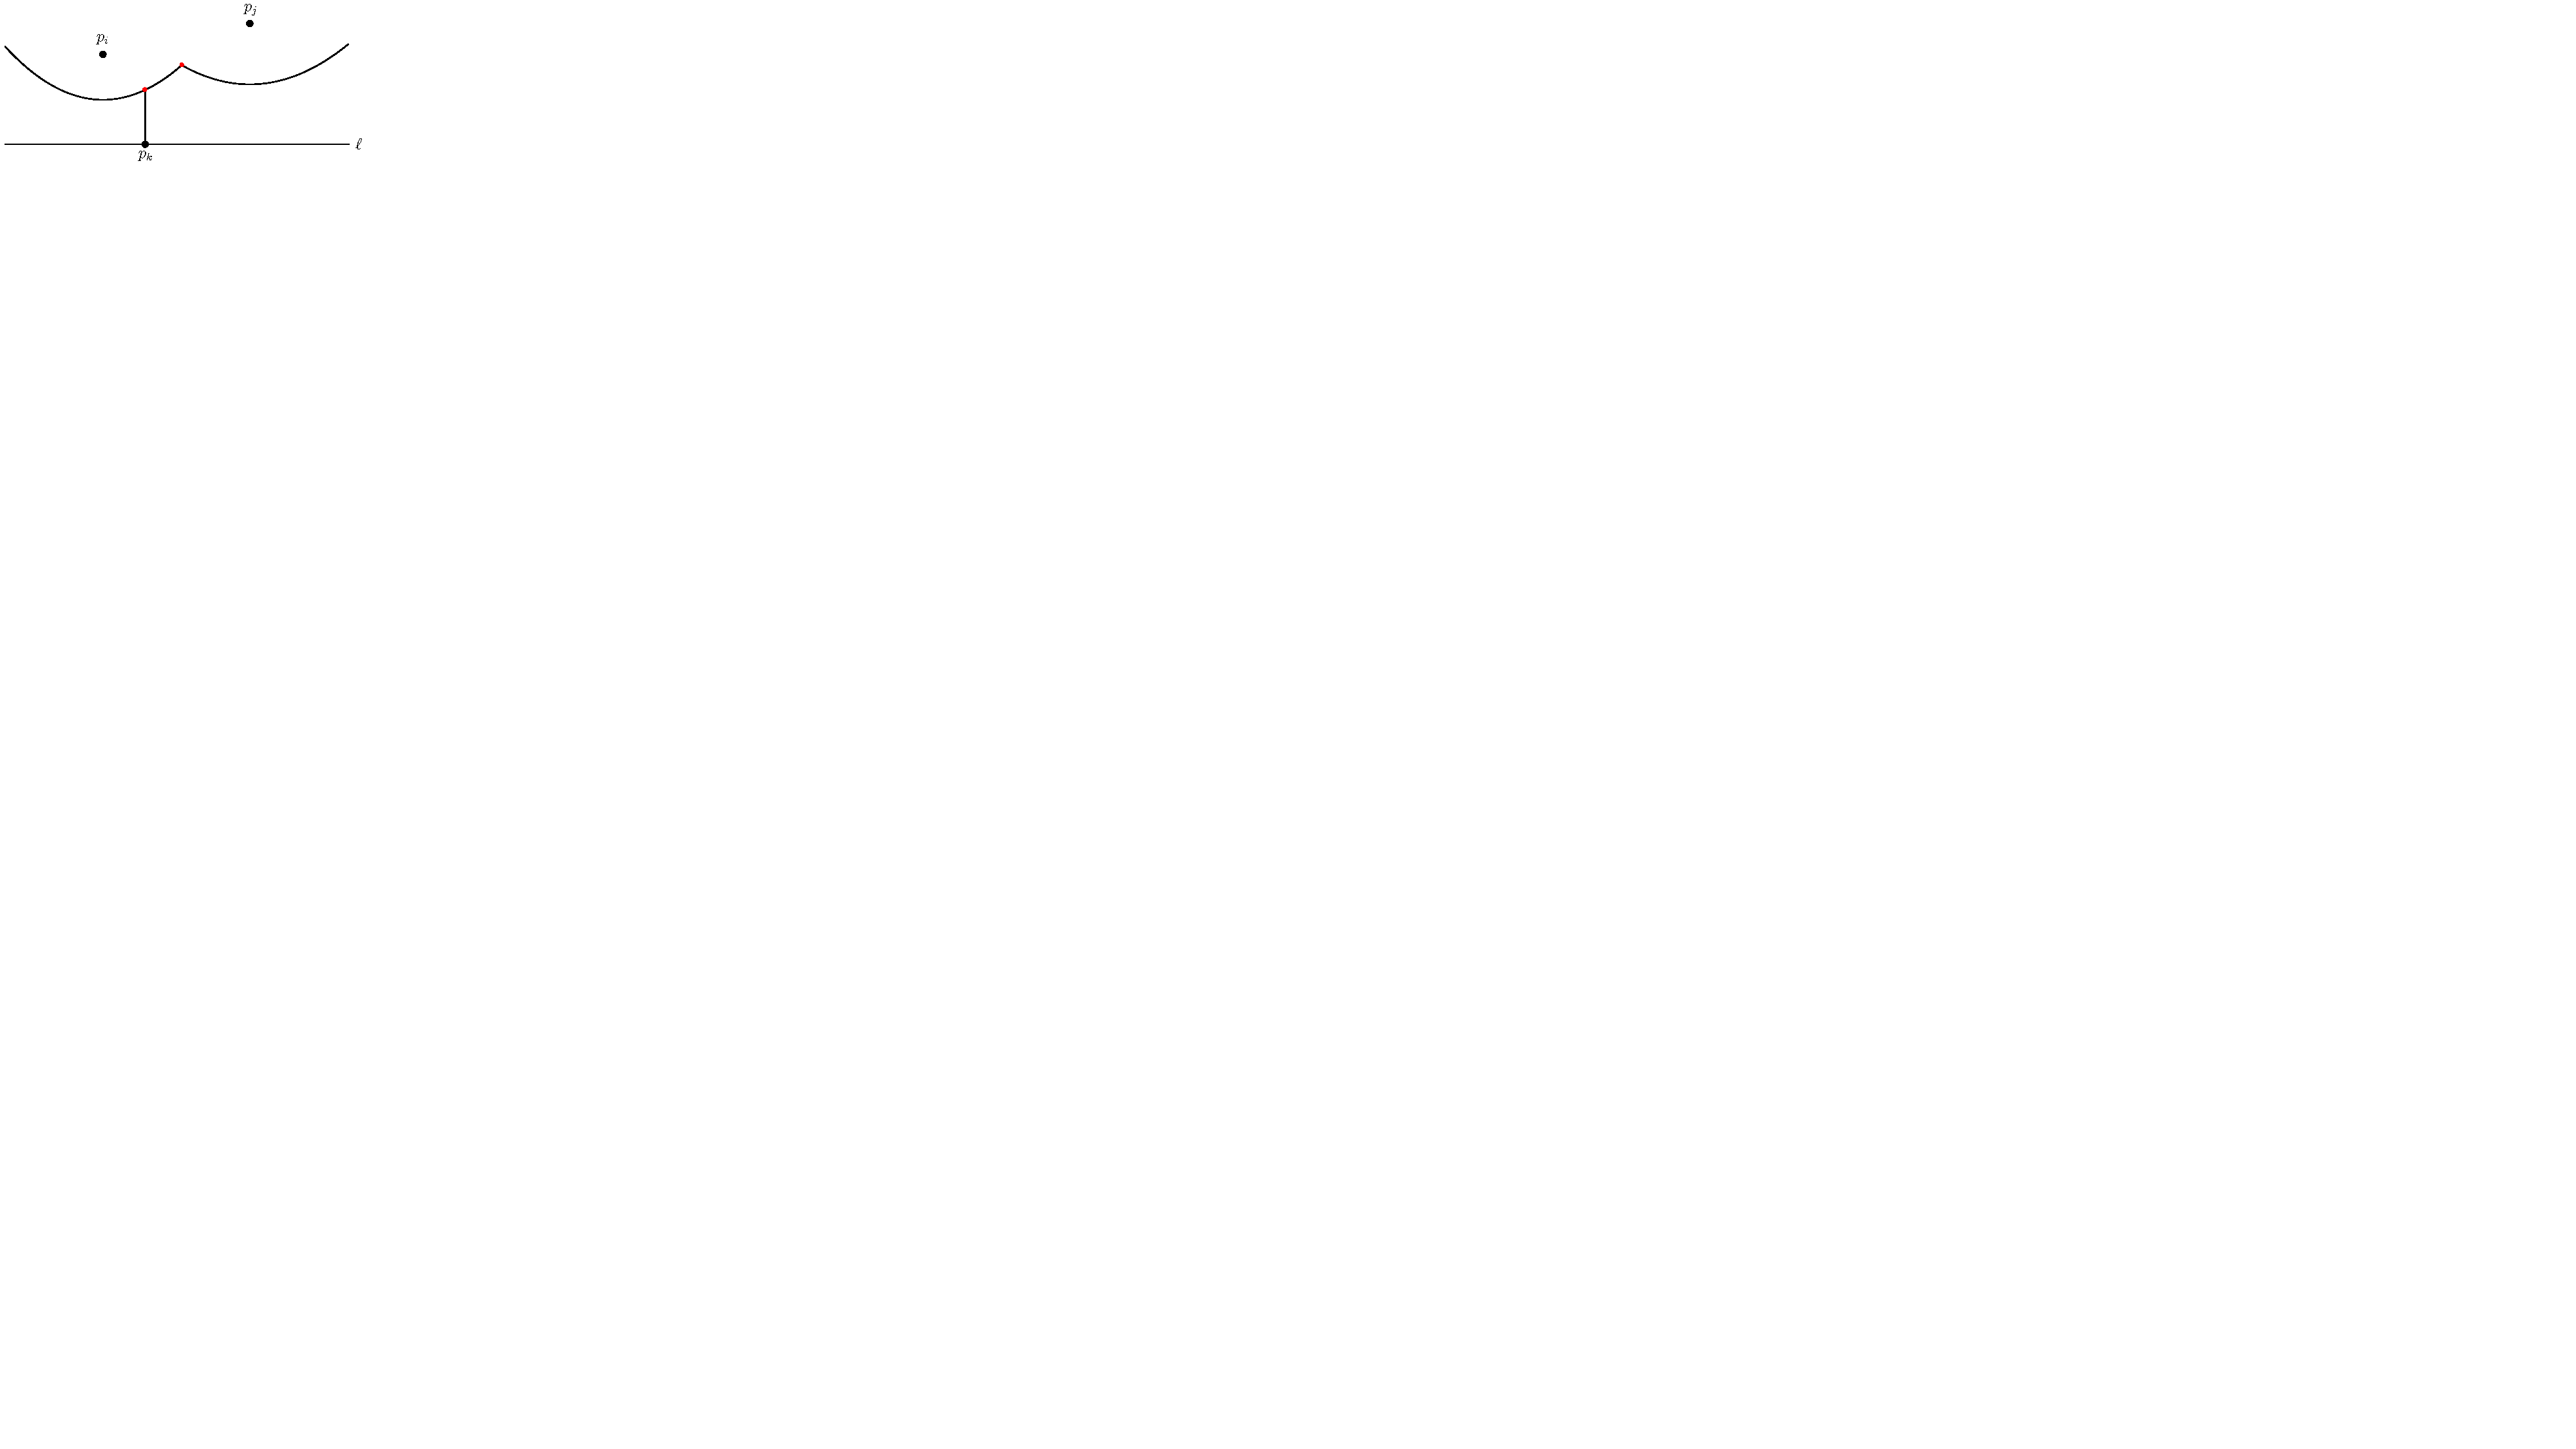
\includegraphics[scale=0.8]{breakpoint} %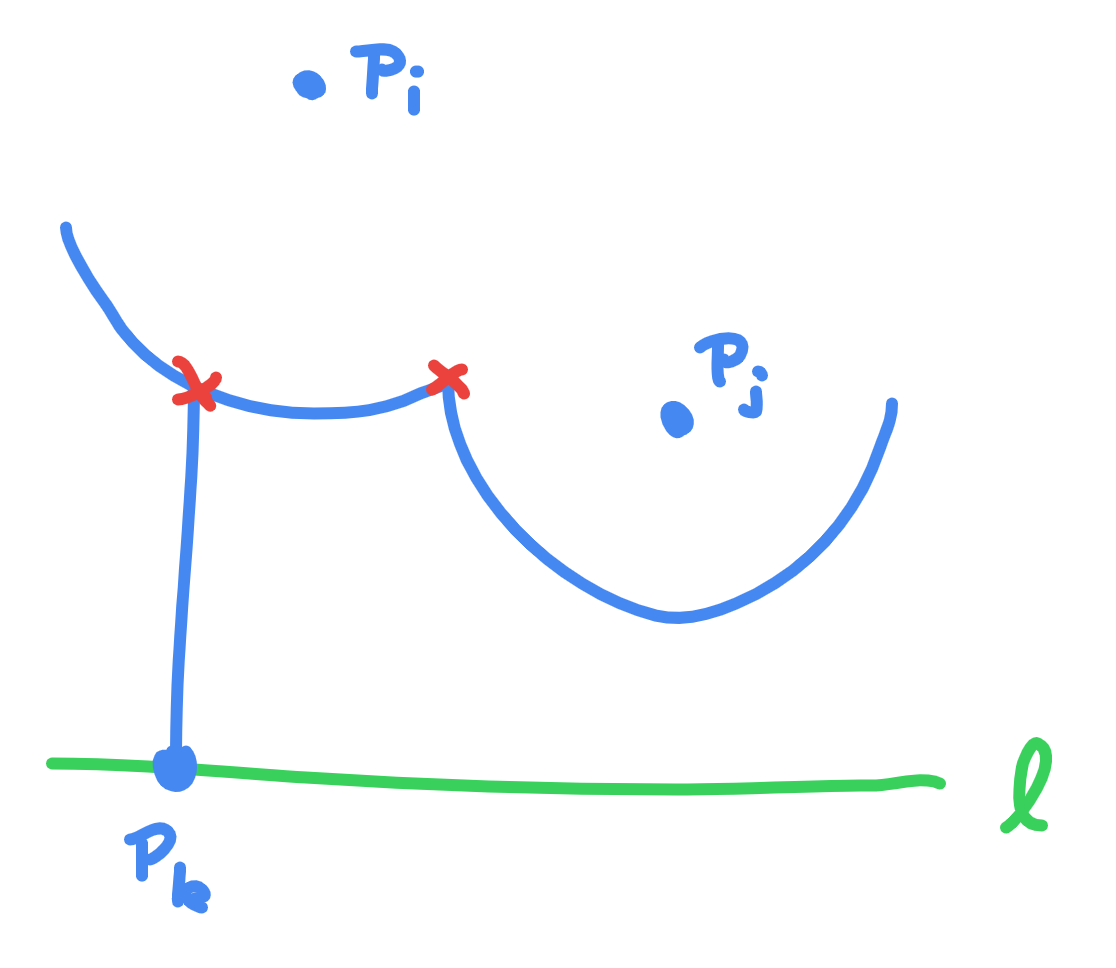
\includegraphics[scale=0.24]{temp-fig-6}
    \caption{The red dots indicate the breakpoints.}
    \label{fig:example-of-breakpoint}
\end{figure}

\section{Breakpoints make out the Voronoi diagram}
Now we show that the breakpoints exactly trace out $\VorG(P)$ as the sweep line $\ell$ moves from top to bottom.
\begin{prop}
We have the following:
\begin{enumerate}[{(}i{)}]
\item For every sweep line $\ell$: $y = \ell_y$ each breakpoint lies on $\VorG(P)$.
\item For every point $q$ in $\VorG(P)$ there is a position of the sweep line $\ell$ such that $q$ is a breakpoint.
\end{enumerate}
\end{prop}
\begin{proof}
We prove each statement individually:
\begin{enumerate}[{(}i{):}]
    \item Let $\ell$ be the sweep line, and assume that it has one or more breakpoints. Let $q \in \R^2$ be such a breakpoint. Then $q \in B_i \cap B_j$ for some $i \ne j$, which means that
    \[
        \dist(q, \ell) = \dist(q, p_i) = \dist(q, p_j).
    \]
    The last equality gives us that $q \not\in \mathcal{V}(p_k)$ for all $k$, hence $q \in \VorG(P)$.
    \item Let $q = (q_x, q_y) \in \VorG(P)$. Since $q$ is either an edge or a vertex, Theorem \ref{thm:characterizationofbisectors} gives us that $\partial C_P(q) \cap P$ has at least two elements, so let $p_i, p_j \in \partial C_P(q) \cap P$ be two different elements. We have $\dist(q, p_i) = \dist(q, p_j)$ by definition of $C_P(q)$, and then we may set
    \[
        \ell_y := q_y - \dist(q, p_i),
    \]
    and obtain
    \[
        \dist(q, \ell) = \dist(q, p_i) = \dist(q, p_j).
    \]
    Then $B_i$ and $B_j$ intersect at $q$, and $q$ is on the beach line since there is no $B_k$ with a point $p_k$ closer to $q$ than $p_i$ and $p_j$, by definition of $C_P(q)$.
\end{enumerate}
\end{proof}

\section{Site and circle events}
As the sweep line $\ell$ sweeps the plane from top to bottom, the combinatorial structure of the beach line changes. We'll categorize these changes into \emph{events}.

First we will consider when new arcs appear on the beach line. As $\ell$ sweeps down and hits a point, a vertical segment is added to the beach line, and then as $\ell$ continues to move, the vertical line spreads out into a new parabolic arc, as seen in this figure:
\[
    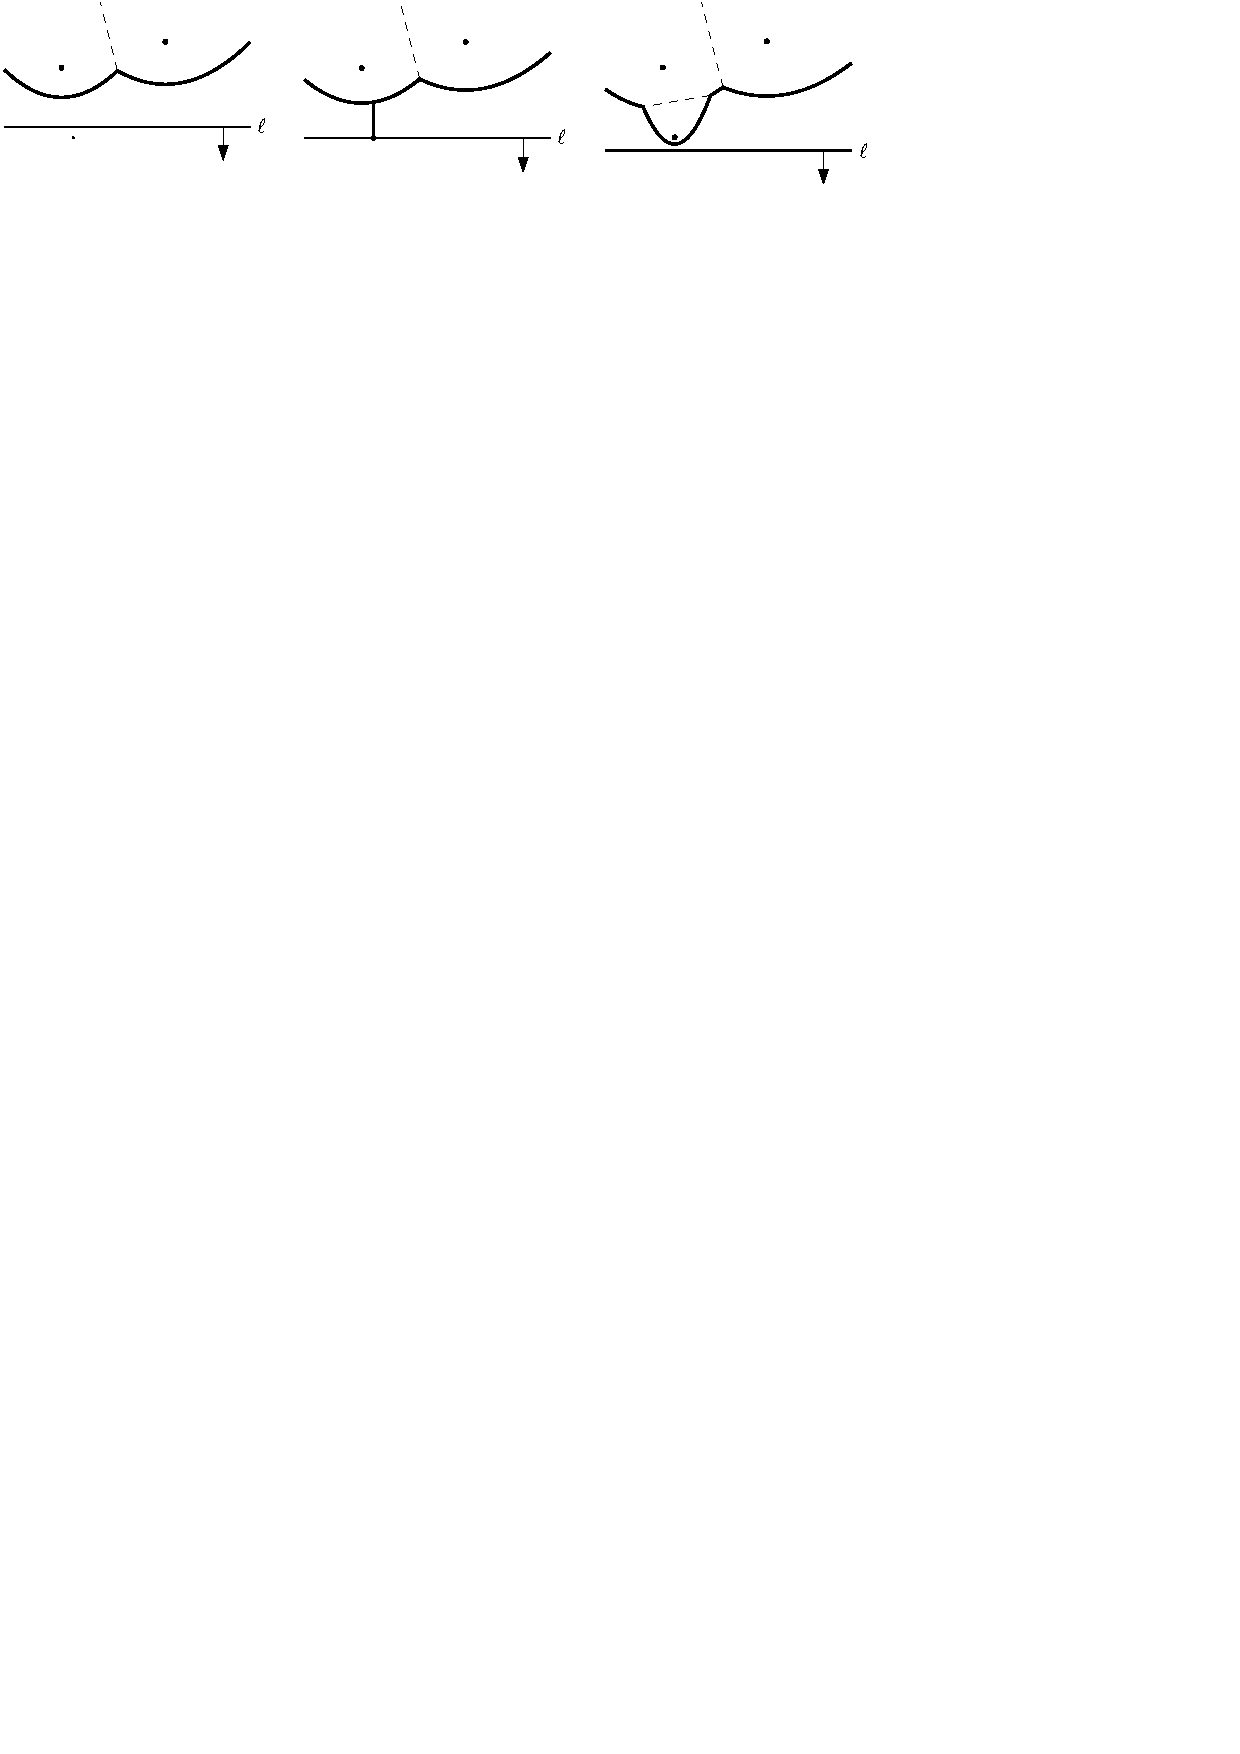
\includegraphics[width=\textwidth]{siteevent} % 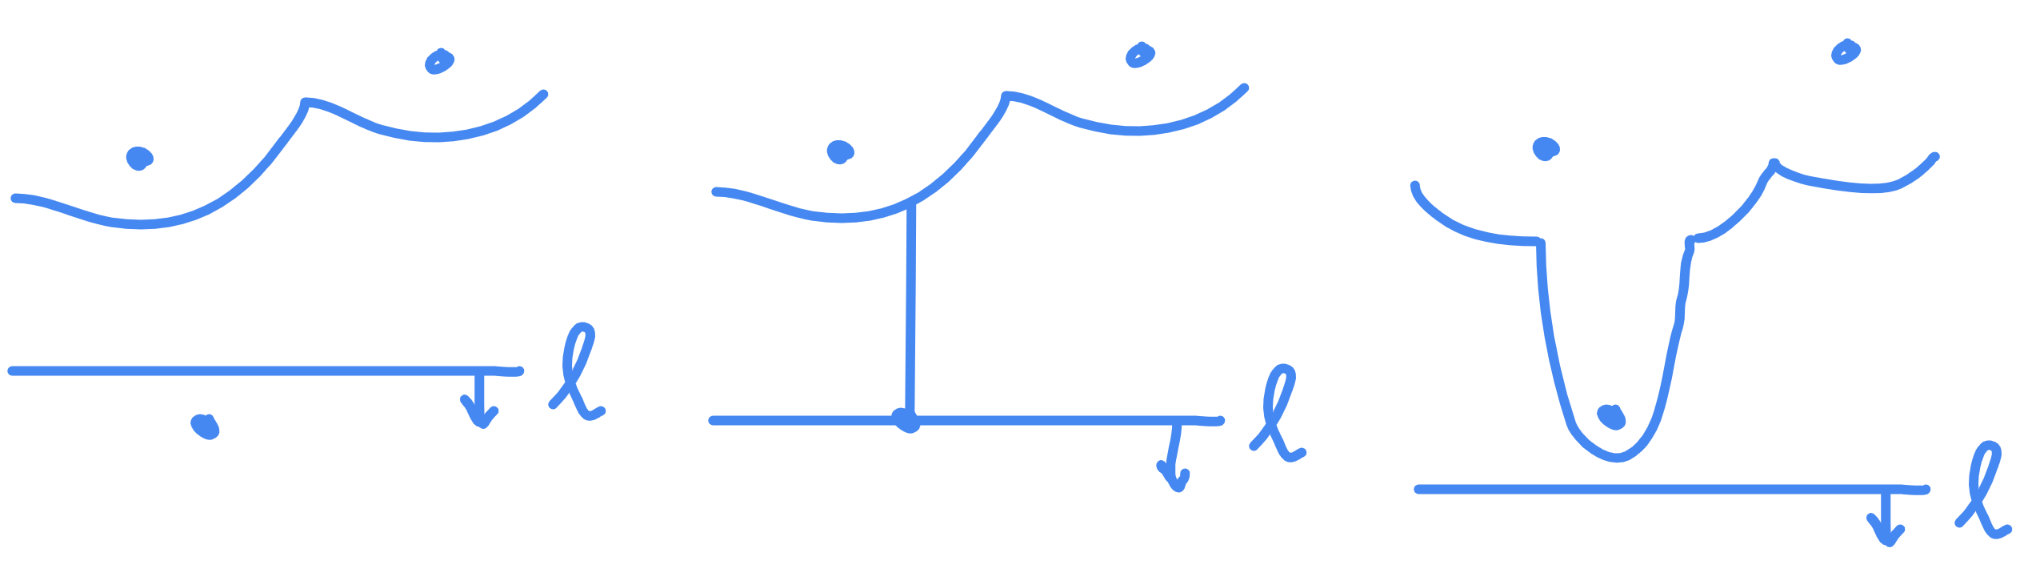
\includegraphics[scale=0.25]{temp-fig-7}
\]
\begin{defn}[Site event]
When $\ell$ encounters a point $p_i \in P$, that is when $\ell_y = (p_i)_y$, we say that we encounter a \emph{site event}.
\end{defn}
\begin{lem} \label{lem:newarciffsiteevent}
The only way in which a new arc can appear on the beach line is through a site event.
\end{lem}
\begin{proof}
The only other alternative is for new arcs to arise due to changes in the shape and position of existing parabolas, that is due to some parabola overtaking the beach line and breaking through it. Assume for the sake of a contradiction that a new arc appears on the beach line but $\ell_y \ne p_i$ for all $i$. Let $\beta_j$ denote the parabola which contains the new arc, associated to the point $p_j \in P$, which appears on the beach line. We have that $\beta_j$ is a full parabola since $\ell_y \ne p_j$. Now, we look at the two cases in which $\beta_j$ can appear as a new arc on the beach line.

The first possibility is that $\beta_j$ breaks through the middle of an another arc which is a part of the parabola $\beta_i$. For this to happen, there is a time at which $\beta_i$ and $\beta_j$ either coincide, or they are tangent which means they intersect in exactly one point which is on the beach line. They cannot coincide, since $p_i \ne p_j$, so they must intersect in exactly one point. By Assumption \ref{ass:generalposition} we have $(p_i)_y \ne (p_j)_y$ so $\beta_i(x) - \beta_j(x)$ is a second degree polynomial with discriminant
\begin{equation}
    D = \frac{(p_x - q_x)^2 + (p_y - q_y)^2}{(p_y - \ell_y)(q_y - \ell_y)}.
\end{equation}
Since $p_y, q_y > \ell_y$ the denominator is strictly positive, and since $p_i \ne p_j$ the numerator is also strictly positive, so $D > 0$. This means that $\beta_i$ and $\beta_j$ intersect in two different points, a contradiction.

The second possibility is that $\beta_j$ appears in between two arcs. Let these arcs be part of parabolas $\beta_i$ and $\beta_k$. Let $q$ be the intersection point between $\beta_i, \beta_j$ and $\beta_k$, and we assume that the arc on the beach line from $\beta_i$ is to the left of $q$, and the arc from $\beta_k$ is to the right of $q$, as in this figure:
\[
    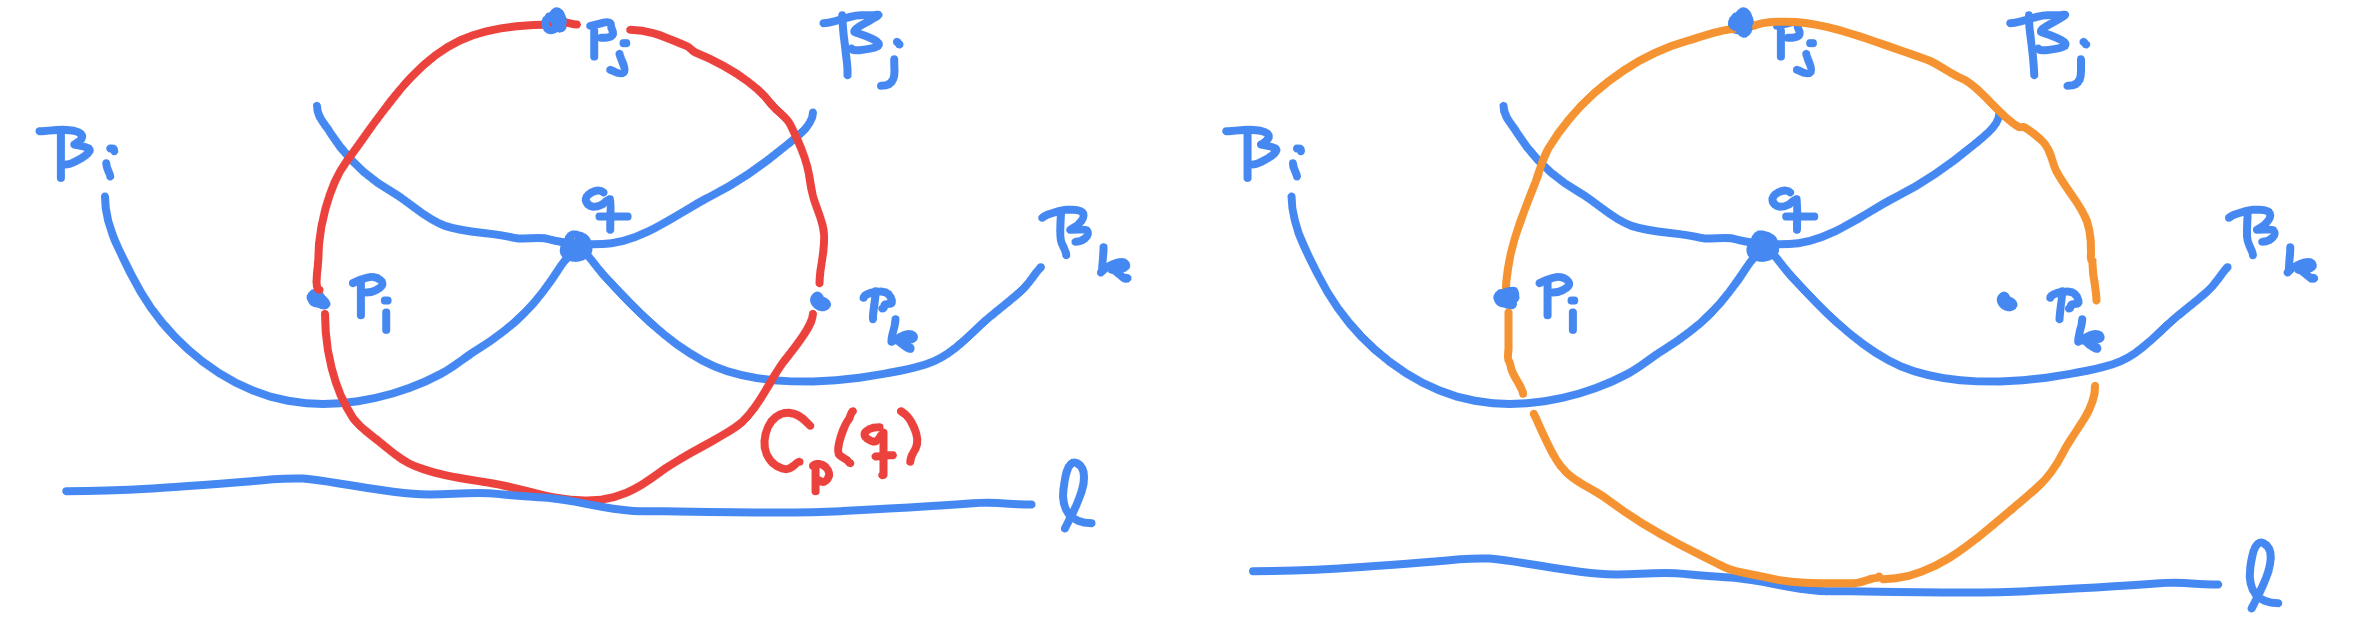
\includegraphics[scale=0.25]{temp-fig-8}
\]
Now let $C$ denote the circle $C_P(q)$ and note that it has $p_i, p_j, p_k$ on its boundary, and it is tangent to $\ell$. The cyclic order on $C$, starting at the point of tangency with $\ell$ and going clockwise is $p_i, p_j, p_k$. Now, we imagine an infinitesimal downward motion of $\ell$ while keeping $C$ tangent to $\ell$ and $p_j$, we call the new circle $C'$. Now either $p_i$ or $p_k$ will be contained in the interior of $C'$, say it's $p_k$ like on the figure. Let $c$ denote the center of $C'$. Then $\dist(c, p_j)$ is equal to $\dist(c, \ell)$, but since $p_k$ is contained in the interior of $C'$ then $\dist(c, p_k)$ is strictly smaller than $\dist(c, p_j)$, which means that $p_k$ is closer to $\ell$ than $p_j$, which means $\beta_j$ cannot be on the beach line, a contradiction.
\end{proof}

\begin{cor}
At any time the beach line consists of at most $2n-1$ arcs.
\end{cor}
\begin{proof}
We prove this by induction. The first site event adds a single arc, so for $n = 1$ there is at most $2n - 1 = 1$ arcs on the beach line. Now assume during the execution of the algorithm that we've seen $k < n$ of the $n$ site events, and that the beach line consists of at most $2k - 1$ arcs. When we encounter a new site, we have seen that there are two cases:
\[
    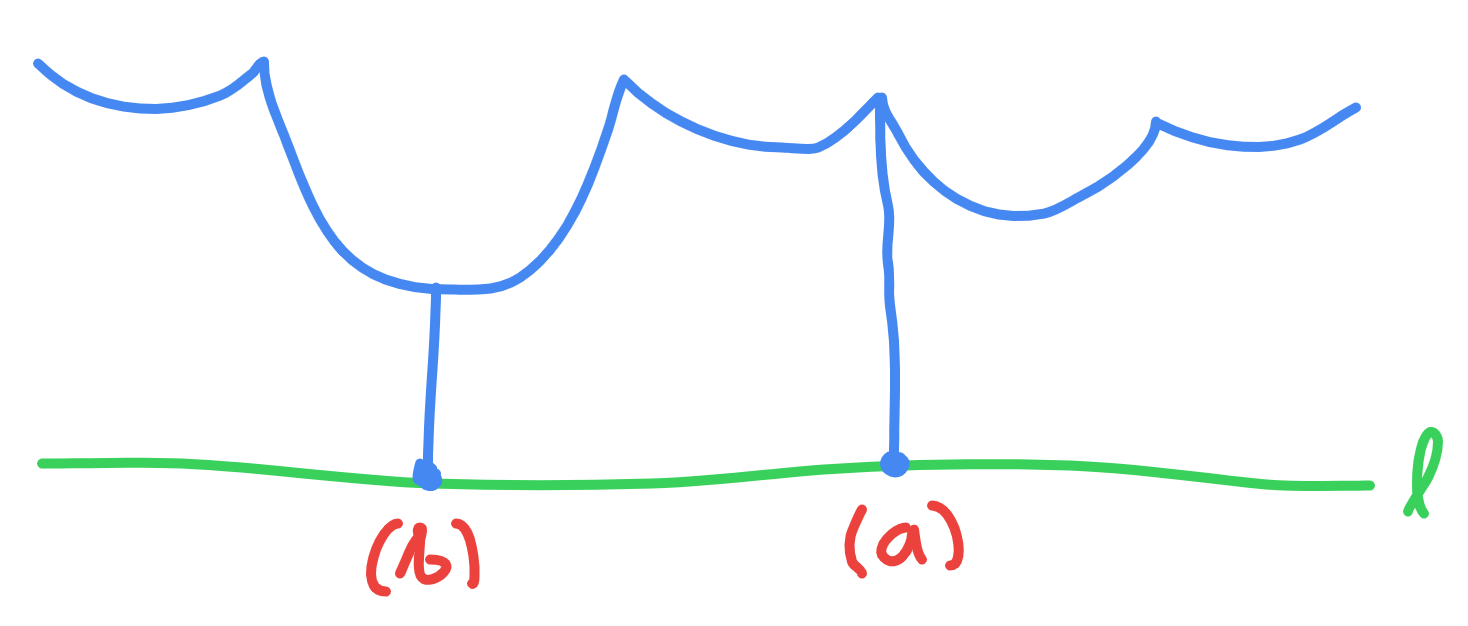
\includegraphics[scale=0.25]{temp-fig-11}
\]
In case (a) the have that an arc appears inbetween 2 existing arcs, increasing the total number by one. In case (b) an existing arc is split into two, and a new arc appears in between, which increases the total number by two. This means that after having seen $k + 1$ site events, there can be at most
\[
    (2k - 1) + 2 = 2(k + 1) - 1
\]
parabolic arcs, which proves the claim.
\end{proof}
Now we've characterized exactly when new arcs appear on the beach line. We now turn to the question of when arcs disappear from the beach line. Assume we have at least 3 arcs on the beach line, name them $\alpha, \alpha', \alpha''$ and assume that $\alpha$ is adjacent to $\alpha'$, and $\alpha'$ is adjacent to $\alpha''$. We assume that $\alpha'$ is the arc which is about to disappear. We first note that $\alpha$ and $\alpha''$ cannot be a part of the same parabola. If this case the case, we'd be in the following situation:
\[
    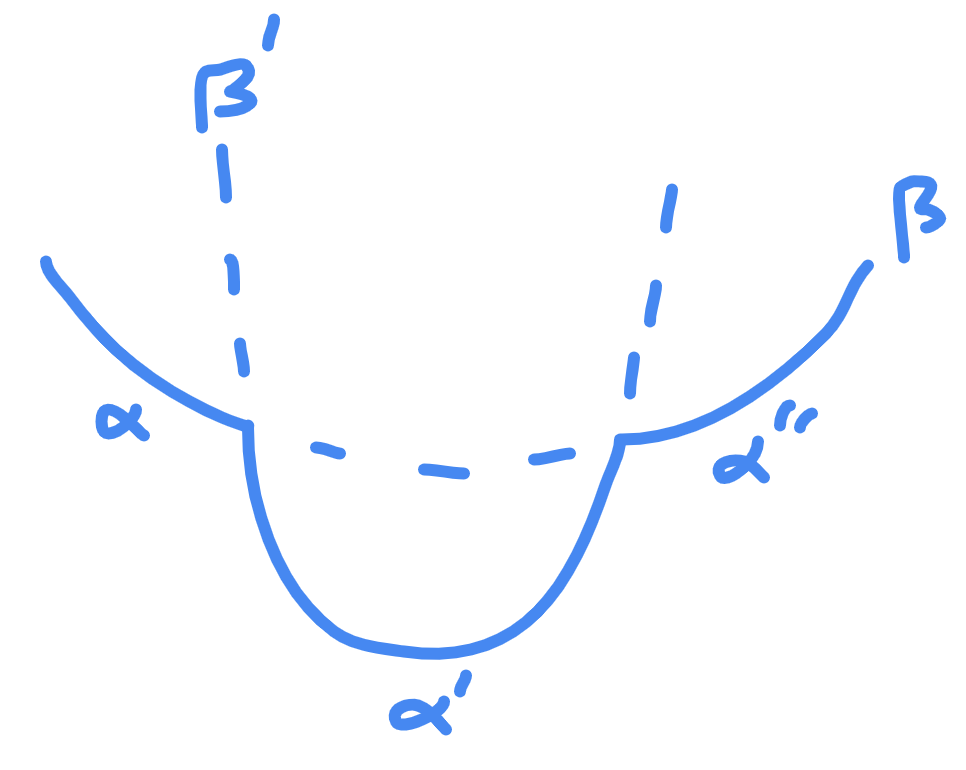
\includegraphics[scale=0.25]{temp-fig-12}
\]
Let $\beta$ denote the parabola which $\alpha$ and $\alpha''$ are a part of, and let $\beta'$ be the parabola which $\alpha'$ is a part of. When $\alpha'$ is about to disappear, then there will be a time at which $\beta$ and $\beta'$ are tangent, and then we can reuse the contradiction argument from the first part of the proof of Lemma \ref{lem:newarciffsiteevent}. Thus $\alpha, \alpha'$ and $\alpha''$ are defined by 3 distinct sites $p_i, p_j, p_k \in P$. At the moment that $\alpha'$ disappears, then the three parabolas $\beta_i \supset \alpha$, $\beta_j \supset \alpha'$ and $\beta_k \supset \alpha''$ intersect in a single point $q$. We note that
\[
    \dist(q, \ell) = \dist(q, p_i) = \dist(q, p_j) = \dist(q, p_k).
\]
So there is a circle $C$ with center $q$ passing through $p_i, p_j, p_k$ which is tangent to $\ell$ at its lowest point. The situation is illustrated as follows:
\[
    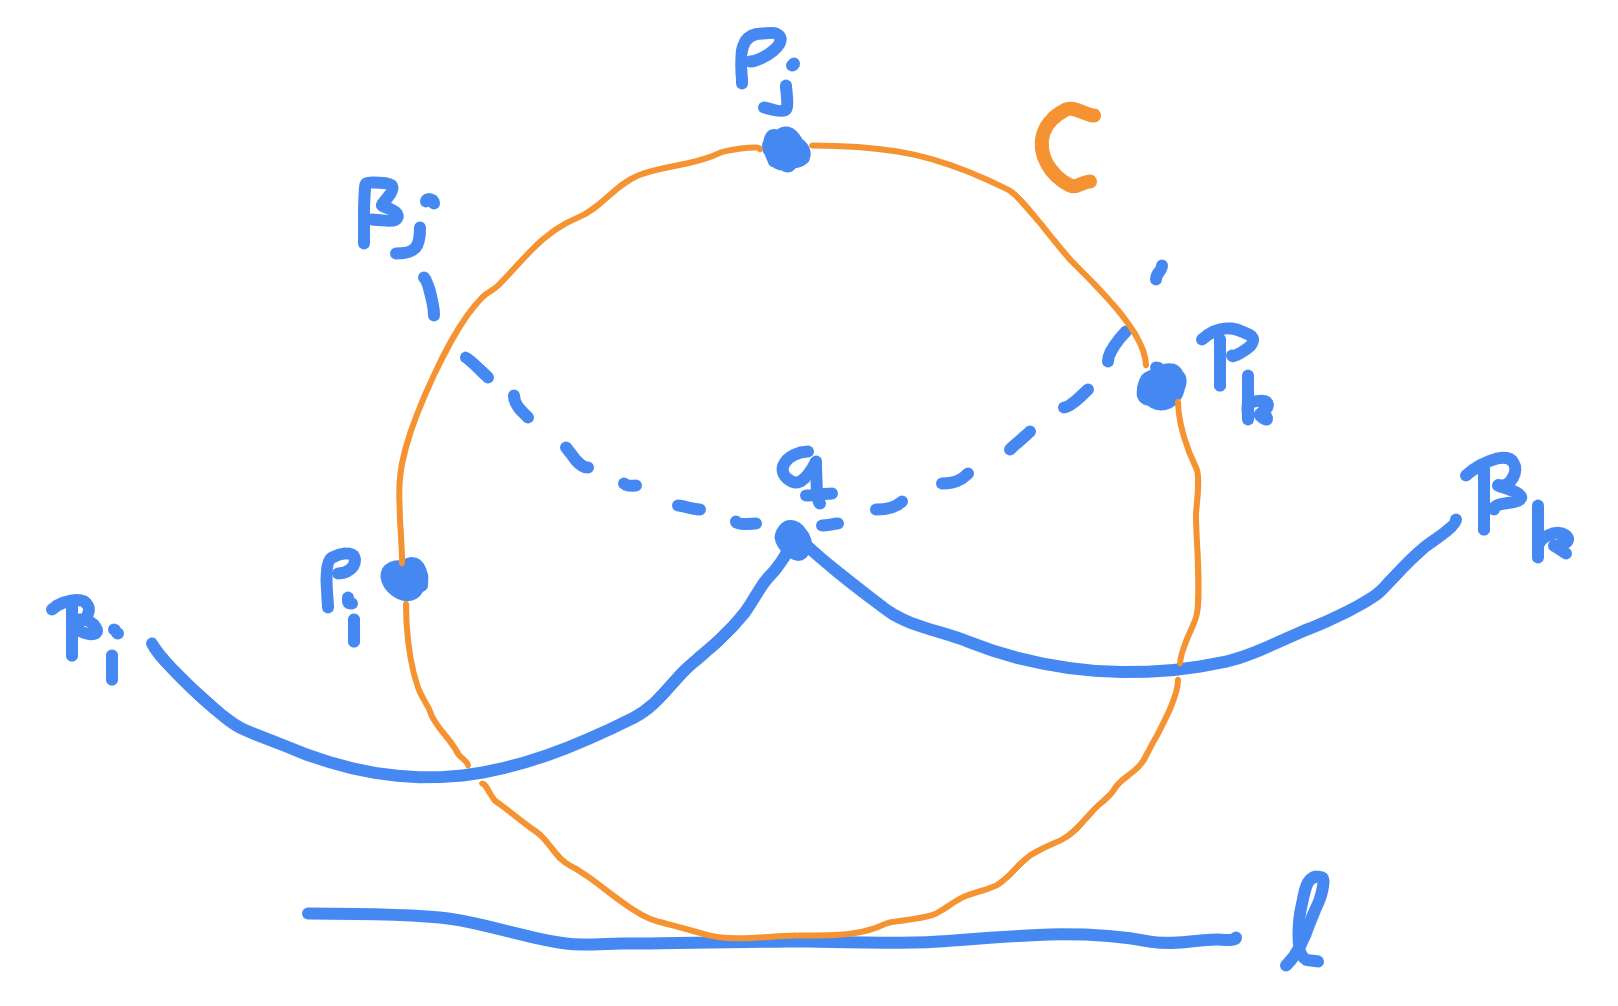
\includegraphics[scale=0.25]{temp-fig-13}
\]
We claim that $C = C_P(q)$. Assume for the sake of a contradiction that there is a site $p$ inside the interior of $C$. Then
\begin{equation} \label{eq:notonthebeachlinechar}
    \dist(p, q) < \dist(q, \ell).
\end{equation}
Now note the following characterization of being on the beach line: A point $r$ is on the beach line if $\dist(r, \ell) = \dist(r, p_i)$ for all $i \in \mathcal{I}$ and $\dist(r, \ell) < \dist(r, p_j)$ for all $j \in \mathcal{J}$, where $\mathcal{I}$ describes those indices $i$ where $r \in \beta_i$ and $\mathcal{J}$ describes those indices where $r \not\in \beta_j$. By assumption $q$ is on the beach line, since it is a point on all of $\alpha, \alpha', \alpha''$ but (\ref{eq:notonthebeachlinechar}) contradicts the characterization we just gave of the beach line. So it must be the case that $C = C_P(q)$. Now note that
\[
    \curly{p_i, p_j, p_k} \subset \partial C_P(q),
\]
so Theorem \ref{thm:characterizationofbisectors} (i) gives us that $q$ is a vertex of $\VorG(P)$. Compare this to the fact that breakpoints trace out $\VorG(P)$ as we proved earlier. This means that when two breakpoints meet and an arc disappears from the beach line, then two edges of $\Vor(P)$ meet at a vertex. We call the event when $\ell$ reaches the lowest point of a circle through three sites defining consecutive arcs on the beach line a \emph{circle event}. We have thus just proven:
\begin{lem}
The only way in which an existing arc can disappear from the beach line is through a circle event.
\end{lem}

\todo{Prove Lemma 7.8: Every Voronoi vertex is detected by means of a circle event. (p. 157)}
\chapter{Data structures for Fortune's algorithm}

During the algorithm we will need three data structures:
\begin{itemize}
    \item A \textbf{priority queue} $\mathcal{Q}$ for keeping track of the site and circle events.
    \item A \textbf{doubly-connected edge list (DCEL)} $\mathcal{D}$ for keeping track of the current state of the Voronoi diagram. See Definition \ref{defn:dcel}. This will be updated after each site and circle event.
    \item A self-balancing \textbf{binary search tree (BST)} $\mathcal{T}$ for keeping track of the breakpoints and arcs on the beach line.
\end{itemize}
We explain them in detail in the next sections.

\section{Priority queue}
The priority queue stores the site and circle events, and enables the algorithm to handle them in order. Each element in the priority queue has a priority. For a site event the $y$-value of the point describes the priority, and for a circle event the priority is given by the $y$-value of the lowest point of the center of the circle which describes the event. Site events also store a pointer to the site, and circle events also store the center of its definining circle and a pointer to the arc in $\mathcal{T}$ which is disappearing.

For the implementation of the priority queue we will use a binary heap. These are described in CLRS \todo{Ref}, and the implementation has been taken from \todo{Ref}.

\section{Binary search tree}
We will store the current configuration of the beach line in a binary search tree, which has some additional information stored:
\begin{itemize}
    \item Leaves correspond to arcs on the beach line. Every leaf has a pointer to a site in $P$, and it also has a pointer to a potential circle event at which the arc will disappear. If no circle event has been detected yet, the pointer will simply be \textsc{nil}. Every arc will also store \textsf{.leftArc} and \textsf{.rightArc} pointers to the two arcs that surround it, so that we get a doubly linked list of arcs that are currently on the beach line. These pointers are \textsc{nil} if the leaf has no neighbour in that particular direction. In our figures the leaves will be depicted by squares.
    
    \item Internal nodes correspond to breakpoints on the beach line. Every breakpoint stores an ordered pair $(p, q)$, where $p$ and $q$ are sites in $P$. The order is important since the intersection of the hyperbolas defined by $p$ and $q$ consists of two points, and the order lets us tell these breakpoints apart. If we consider the beach line as running from the left to the right, then at every breakpoint an arc is leaving, and another is entering it. Thus the tuple $(p, q)$ tells us that we are interested in the breakpoint at which an arc pointing to $p$ leaves, and an arc pointing to $q$ is entering. In our figures the internal nodes will be depicted by circles.
\end{itemize}

The binary tree will only be updated at site and circle events. First we describe what happens at a site event.

\subsection{Inserting at site events} \label{sec:insertingatsiteevents}
During the first site event, the tree will be empty (we say it is \textsc{nil}), so to add an arc $\alpha$ to it, we simply turn the tree into a leaf, which describes the new arc, and we have it point to the first site $p$, illustrated as follows:
\[
    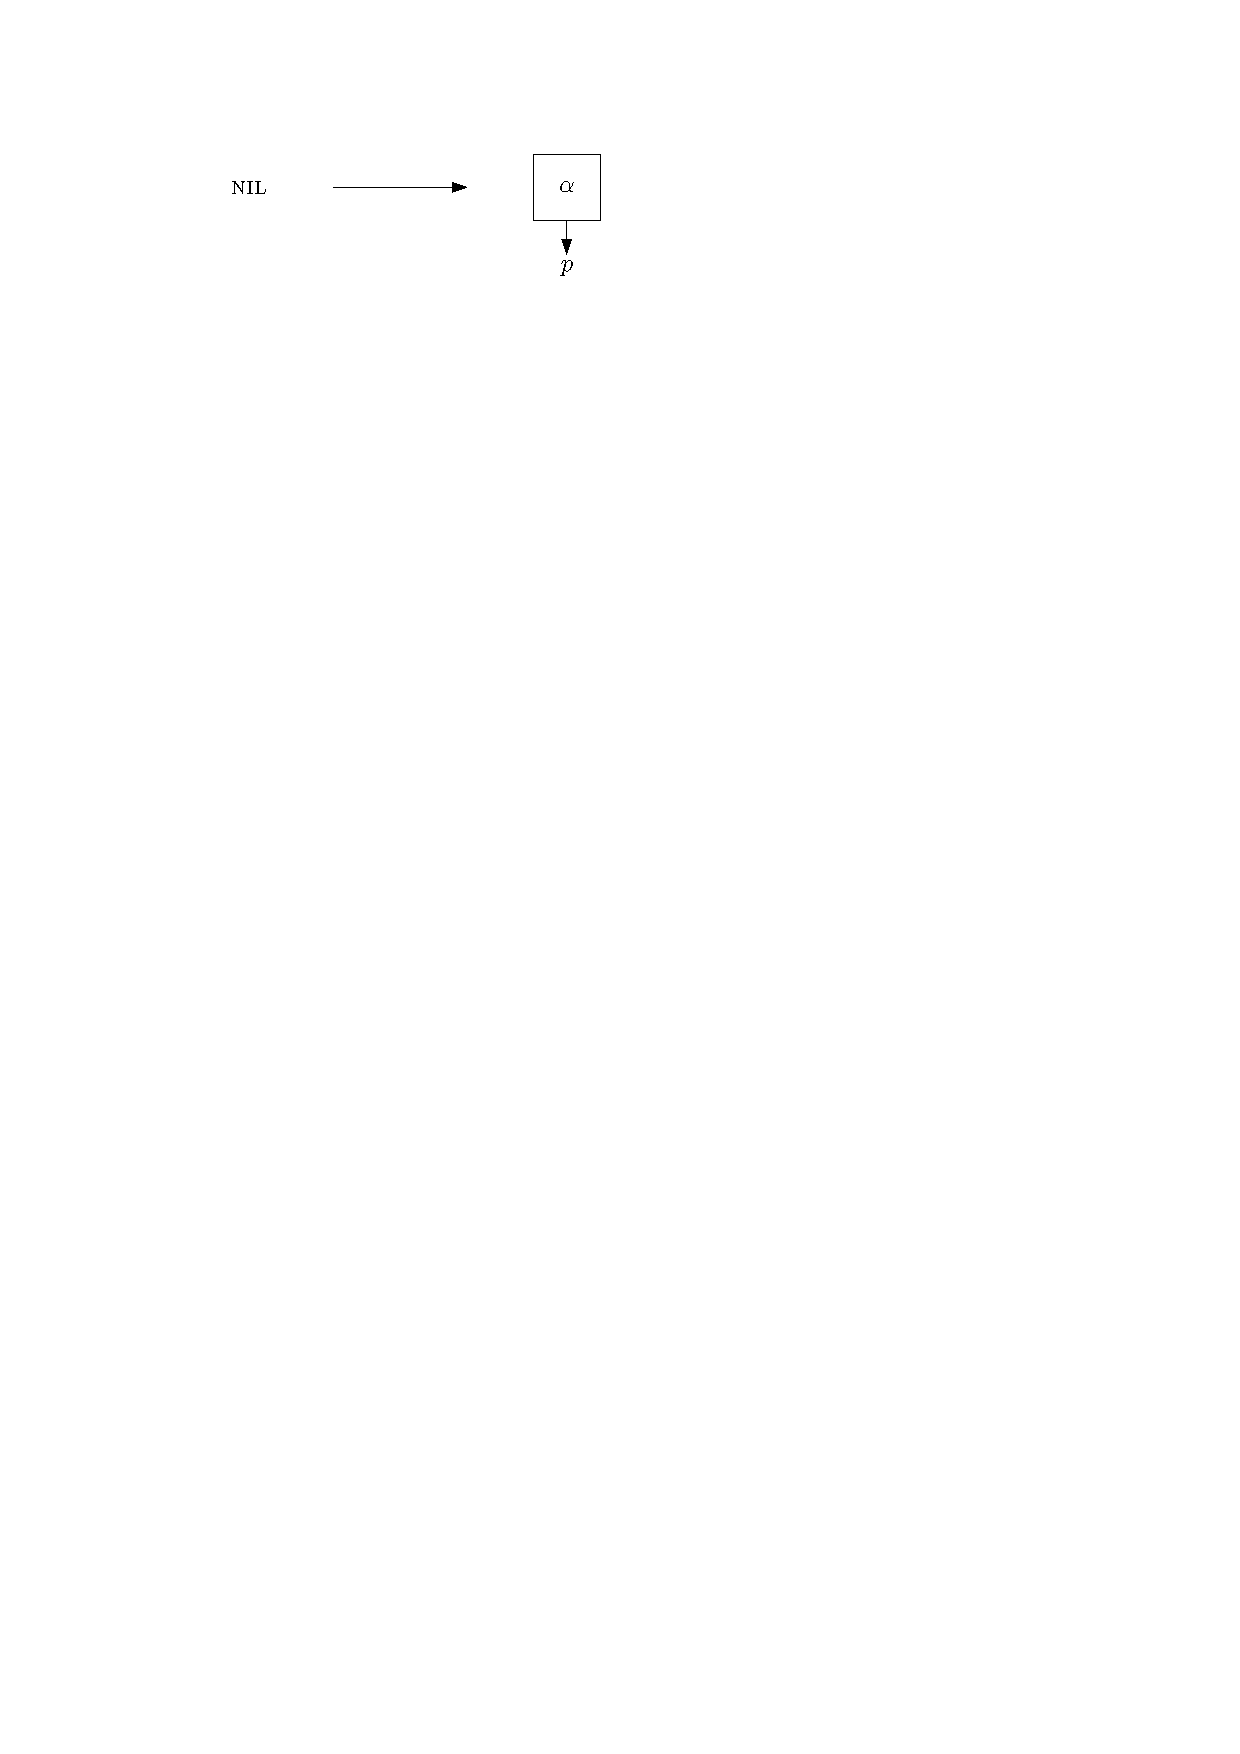
\includegraphics[scale=0.75]{images/tree_insert_base}
\]
Now we look at the general case. We assume that $\alpha$ is an arc on the beach line, which points to a point $p$, and that we at a site event discover a new point $q$ which is located below the arc $\alpha$ (e.g. a vertical line going through $q$ intersects $\alpha$). At this site event, the arc $\alpha$ will be split into two arcs $\alpha_1$ to the left, and $\alpha_2$ to the right, and two breakpoints $x$ and $y$ with $x \leq y$ will be introduced. We update the tree locally as illustrated in the figure below:
\[
    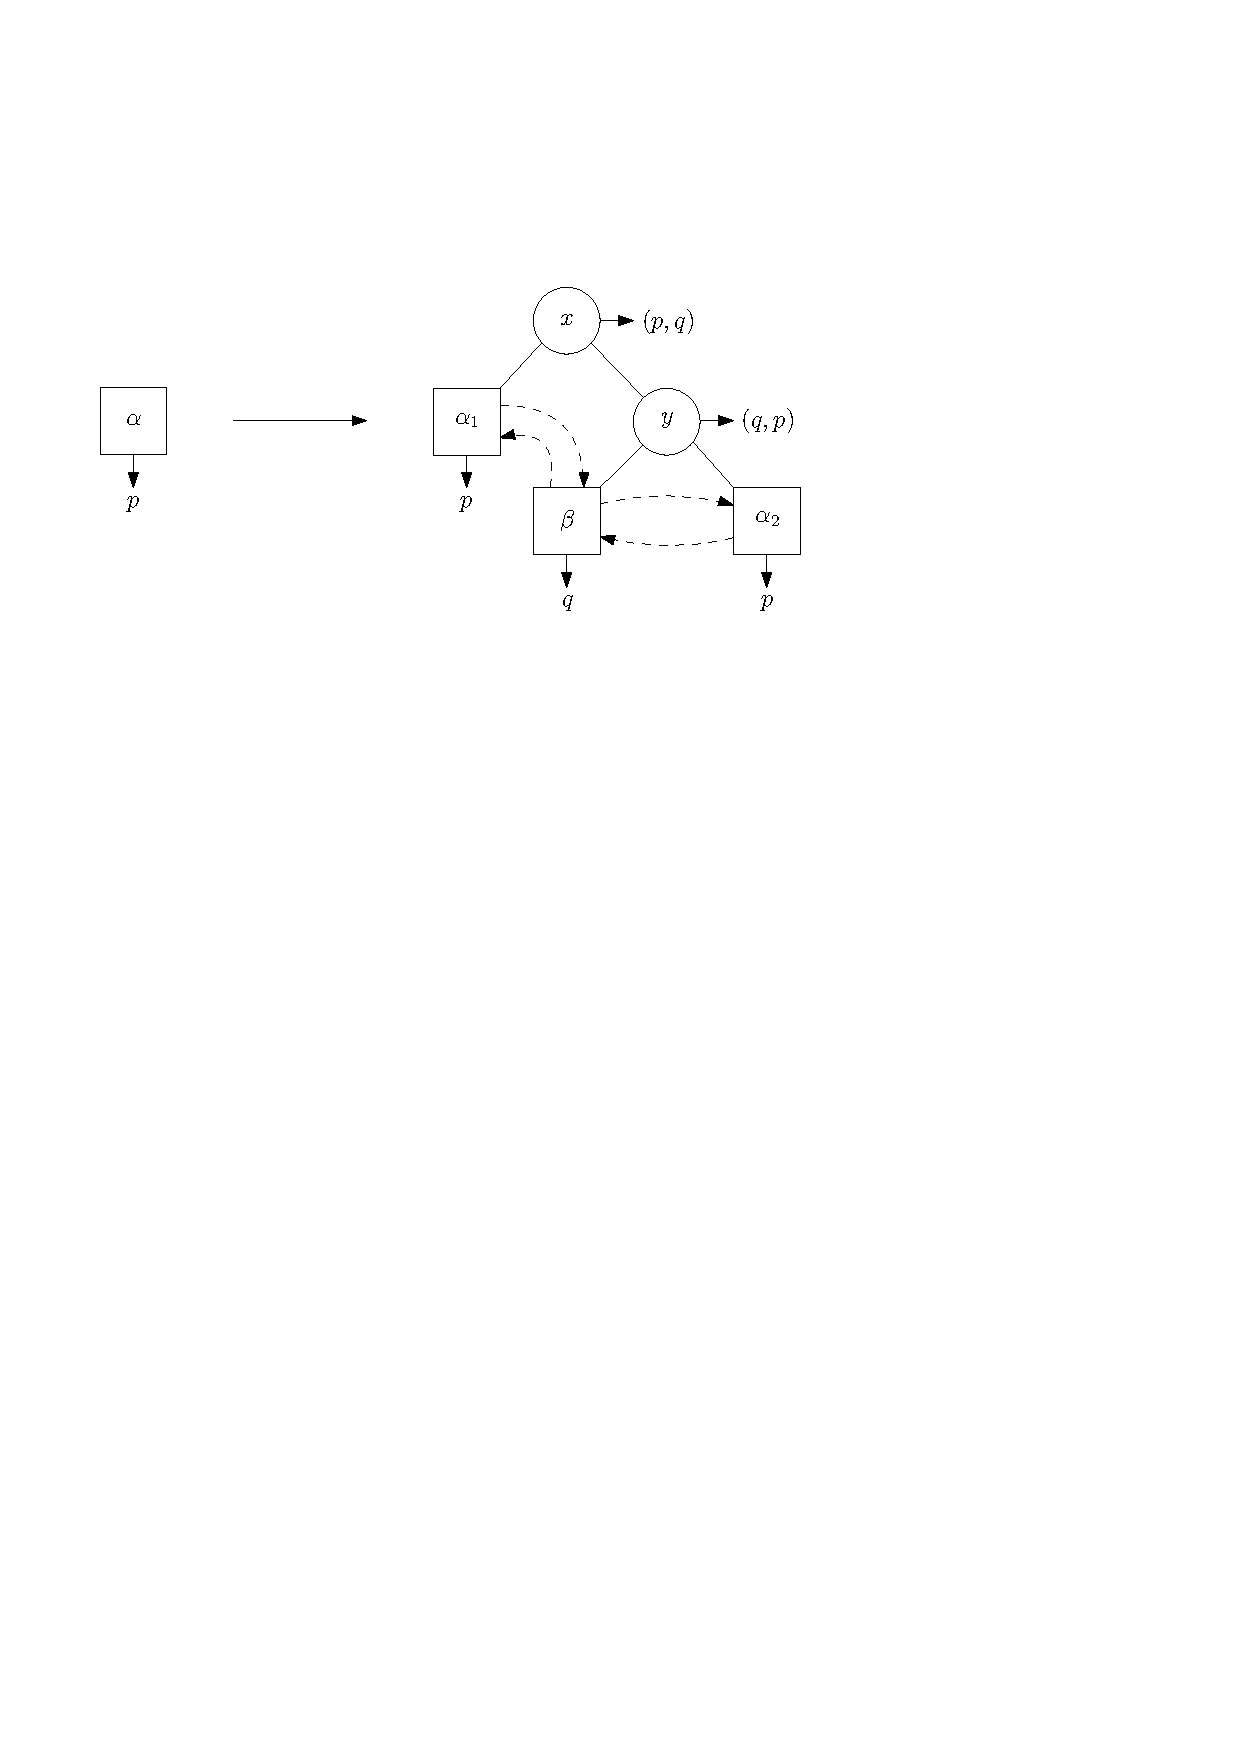
\includegraphics[scale=0.75]{images/tree_insert}
\]
The leaf $\alpha$ gets replaced by the tree on the right. The dashed arrows represent the pointers for our doubly linked lists of arcs, and not depicted but also necessary is that we need to connect $\alpha_1$ to $\alpha$\textsf{.leftArc} and connect $\alpha_2$ to $\alpha$\textsf{.rightArc} by setting the appropriate pointers.

\subsection{Deleting at circle events}
At a circle event two breakpoints $x$ and $y$ converge into a single breakpoint $z$ and an arc $\gamma$ disappears. In terms of the tree we must modify, the fact that the breakpoints $x$ and $y$ are converging means that $y$ is the successor of $x$. What this means for the structure of the tree depends on whether $x$ is an ancestor of $y$, or if $y$ is an ancestor of $x$. First, we assume that $x$ is an ancestor of $y$. Then $y$ is the lowest internal node on the left spine of $x$\textsf{.right}, and our modification is as illustrated:
\[
    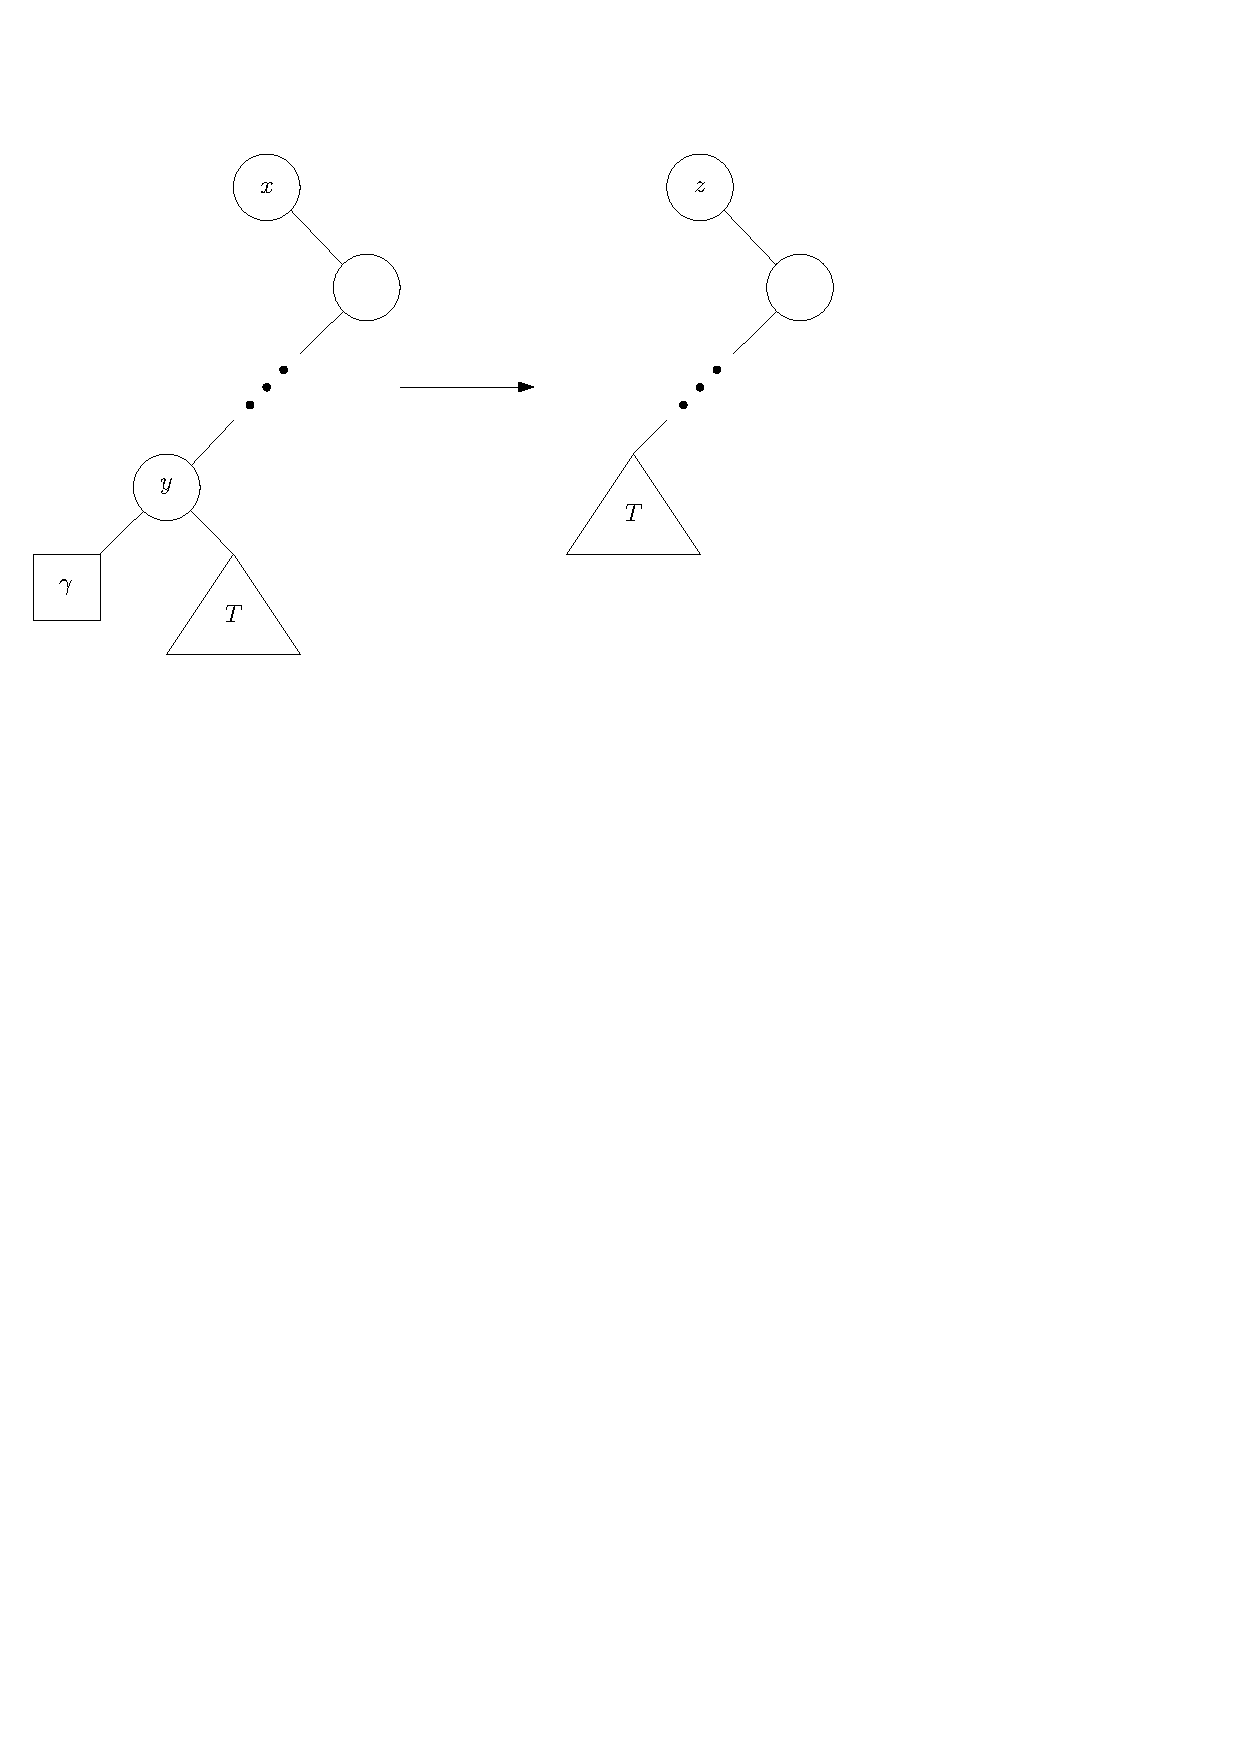
\includegraphics[scale=0.6]{images/tree_remove_xy}
\]
We replace $y$ by $T = y\textsf{.right}$, effectively removing $y$ and $\gamma$. Then we replace $x$ by $z$. This way the tree stays a binary tree, and the new structure of the beach line is now rightfully represented.

On the other hand, if $y$ is an ancestor of $x$, then $x$ is the lowest internal node on the right spine of $y$\textsf{.left}. We then make the following modification:
\[
    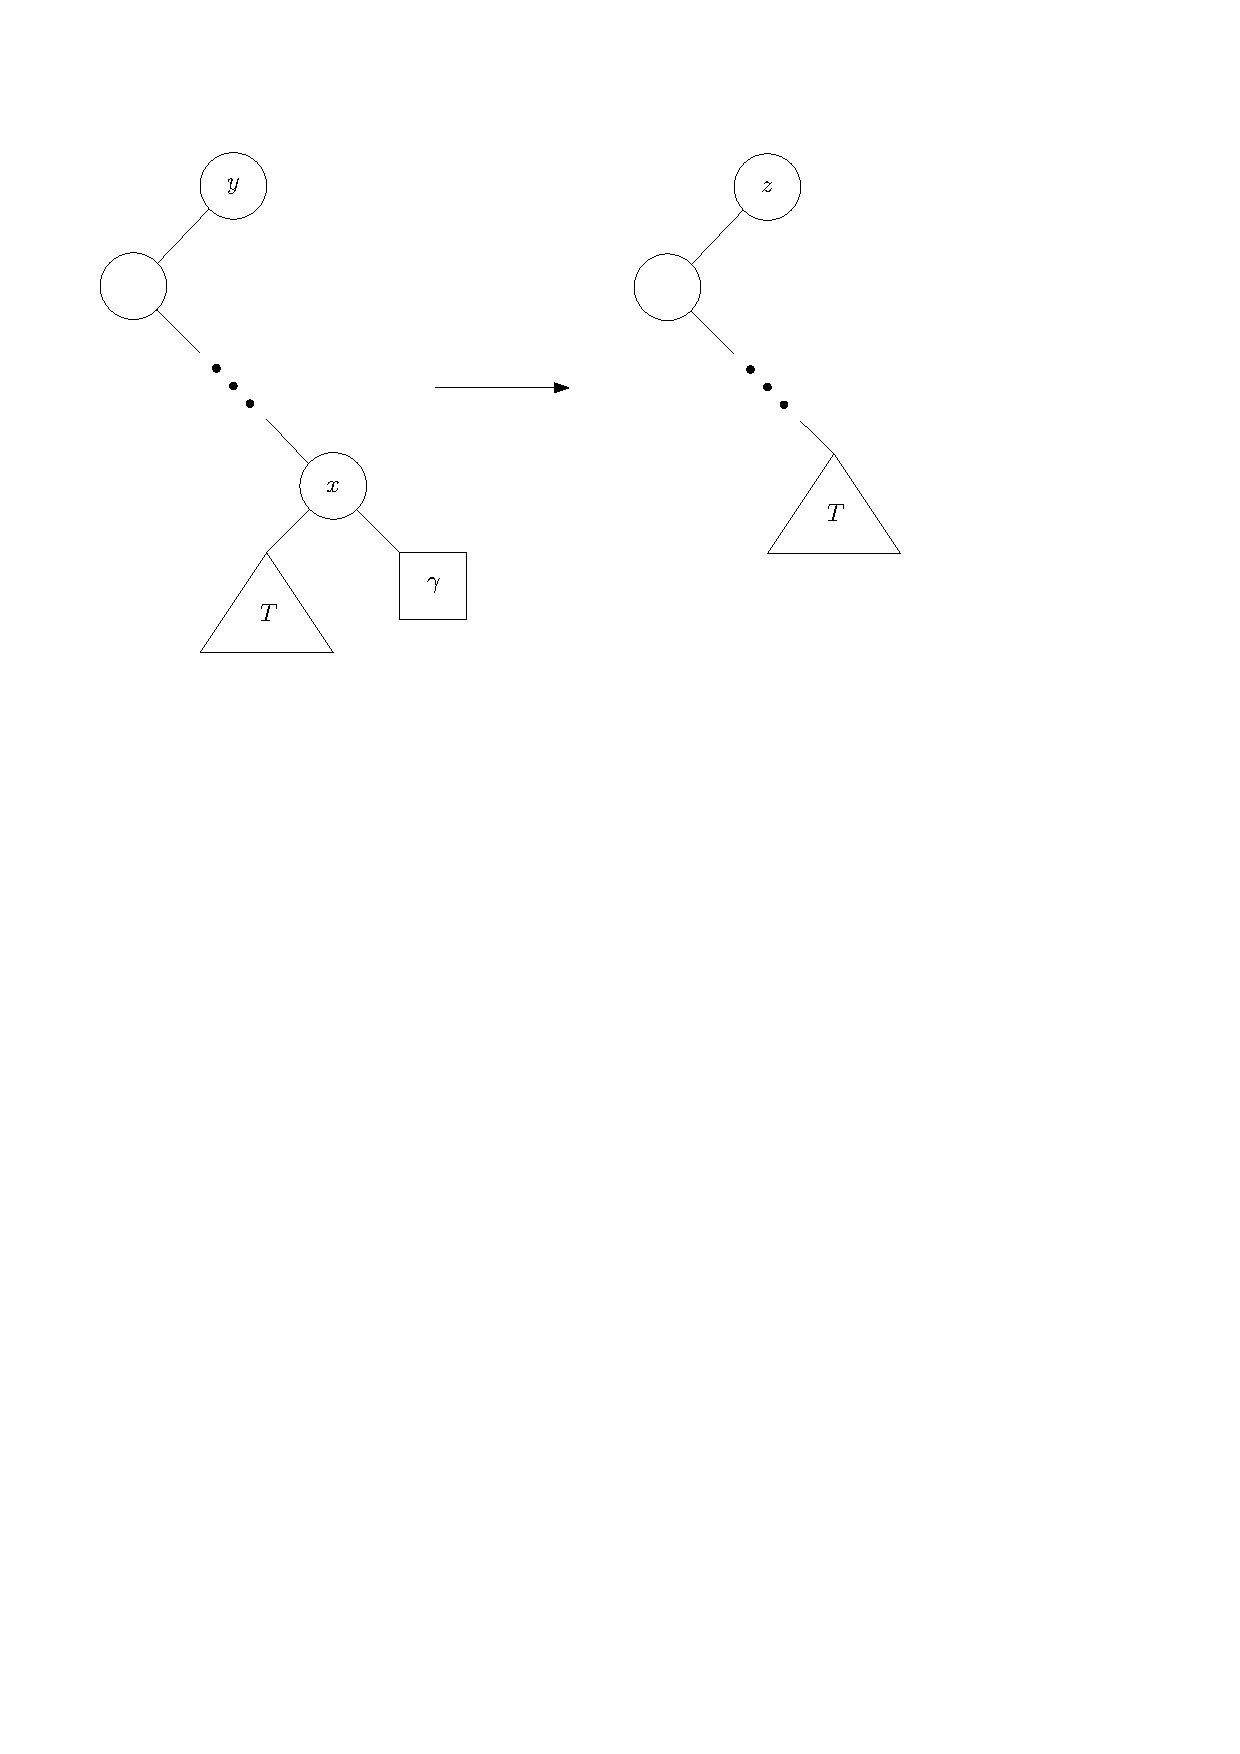
\includegraphics[scale=0.6]{images/tree_remove_yx}
\]
We replace $x$ by $T = x\textsf{.left}$, effectively removing $x$ and $\gamma$. Then we replace $y$ by $z$. Again, this way the tree stays a binary tree, and the new structure of the beach line is now rightfully represented.

We would like the tree to be balanced in order for search to be fast, so we need to balance the tree after inserting and deleting. We'll look at an approach to do this in the next section.

\section{Balancing the BST by using a treap}
There are multiple viable strategies for balancing a binary search tree. In this section we look at a particular strategy which utilizes randomness. We will introduce the treap data structure, which is a randomized self-balancing binary search tree. The presentation follows the paper \todo{Ref}, but only describes the things that we will need.

\begin{defn}[Treap]
Let $T$ be a tree where each node $x \in T$ has properties
\begin{itemize}
    \item $x\textsf{.left}$ is the left subtree of $x$,
    \item $x\textsf{.right}$ is the right subtree of $x$,
    \item $x\textsf{.key} \in \R$,
    \item $x\textsf{.priority} \in [0,1]$.
\end{itemize}
We say that $T$ is a \textit{treap} if
\begin{enumerate}[(i)]
    \item $T$ is a binary tree with respect to $\textsf{.key}$. That is, for every $x \in T$ we have
    \begin{align*}
        \forall y \in x\textsf{.left} &\colon y\textsf{.key} \leq x\textsf{.key}, \\
        \forall y \in x\textsf{.right} &\colon y\textsf{.key} \geq x\textsf{.key}.
    \end{align*}
    \item $T$ is a max-heap with respect to $\textsf{.priority}$, that is for each $x, y \in T$:
    \begin{align*}
        x \text{ is the parent of } y \implies x\textsf{.priority} \geq y\textsf{.priority}.
    \end{align*}
\end{enumerate}
\end{defn}

\begin{defn}[Left and right rotations]
Given a tree $T$ and two nodes $x, y \in T$ with subtrees $A, B, C$ the operations \textit{rotate left} and \textit{rotate right} are given as follows:
\[
    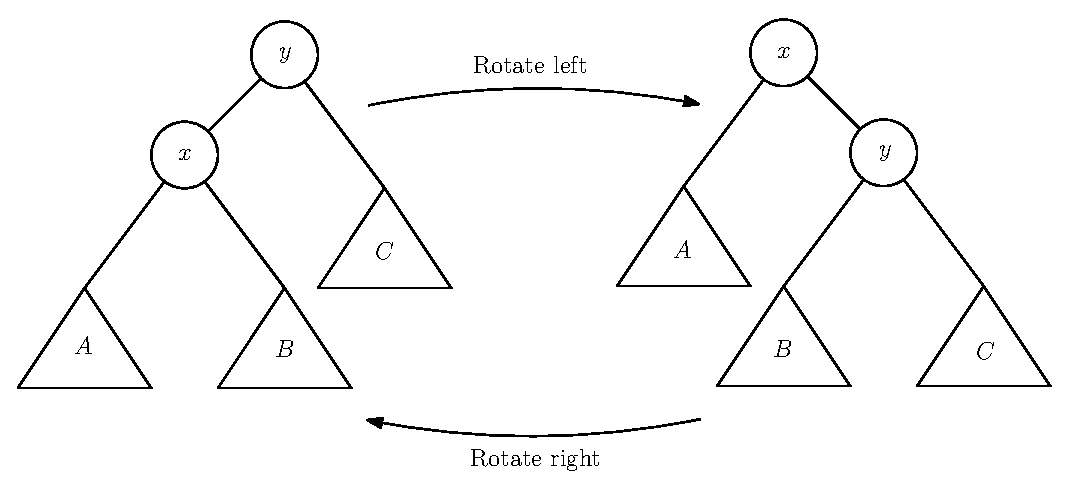
\includegraphics[width=\textwidth]{rotate}
\]
\end{defn}

From the diagram it is immediate that rotations preserve the binary tree property, but if $T$ has a $\textsf{.priority}$ property then the order on $x\textsf{.priority}$ and $y\textsf{.priority}$ is reversed. Given a binary tree $T$ with priorities we may then make sure it also has the max-heap property by making a finite sequence of left and right rotations, and thus we may turn it into a treap.

The basic operations on a treap are as follows:
\begin{itemize}
    \item $\textsc{Search}(x)$: This is the same as for a binary tree.
    \item $\textsc{Insert}(x)$: At first the insertion is identical to that of a binary tree: first we search for a spot to insert the new element, such that it stays a binary tree after insertion. Once inserted however, it may be the case that the max-heap property is violated. To remedy this, we may rotate $x$ up in the tree until the max-heap property is reestablished, or until we reach the root.
    \item $\textsc{Delete}(x)$: The strategy is to rotate $x$ down until it becomes a leaf in a manner which preserves the property that every subtree is a treap, and then we remove the leaf. This is done as follows: when rotating down we have a choice of rotating $x$ with the root $y$ of the left subtree $A$, or the root $z$ of the right subtree $B$. We choose to rotate $x$ and $y$ if $y\textsf{.priority} > z\textsf{.priority}$, otherwise we rotate $x$ and $z$, and then it follows by recursion that the treap property eventually is preserved in the entire tree once $x$ is a leaf, and then we clip away $x$.
\end{itemize}

\begin{defn}[Randomized search tree]
We define a \textit{randomized search tree} to be a treap $T$ where the priorities are independent, identically distributed continuous random variables.
\end{defn}

The main result we will work towards in this section is the following:

\begin{thm} \label{thm:treapmainthm}
A randomized search tree storing $n$ items has the expected performance characteristics listed in the table below:
\begin{table}[h!]
\centering
\begin{tabular}{ll}
\textbf{Performance measure}   & \textbf{Bound on expectation} \\ \hline
Search                         & $\mathcal{O}(\log n)$         \\
Insertion                      & $\mathcal{O}(\log n)$         \\
Deletion                       & $\mathcal{O}(\log n)$         \\
Number of rotations per update & $\leq 2$                      \\ \hline
\end{tabular}
\end{table}
\end{thm}
To prove this we will introduce some random variables and then we will work towards proving upper bounds for their expectations. The first random variables we introduce are:
\begin{itemize}
    \item $D(x)$: the number of nodes on the path from $x$ to the root.
    \item $SL(x)$ and $SR(x)$: the length of the right spine of the left subtree of $x$ and the length of the right spine of the right subtree of $x$. By length of the left spine of a tree we mean the number of nodes we pass if we keep following the left pointer from the root, and similarly for the right spine.
\end{itemize}
Throughout this section we will deal with a treap $T$ with nodes $x_1, x_2, \ldots, x_n$ where node $x_i$ has associated key $k_i$ and priority $p_i$, and $k_1 < k_2 < \cdots < k_n$. We now introduce the following indicator random variables:
\begin{align*}
    A_{i,j} &= \begin{cases}
        1 & \text{if } x_i \text{ is an ancestor of } x_j \text{ in } T, \\
        0 & \text{otherwise.}
    \end{cases} \\
    C_{i;\ell,m} &= \begin{cases}
        1 & \text{if } x_i \text{ is a common ancestor of } x_{\ell} \text{ and } x_{m} \text{ in } T, \\
        0 & \text{otherwise.}
    \end{cases}
\end{align*}
Note that we consider each node an ancestor of itself. We then have:
\begin{thm}
    Let $1 \leq \ell \leq n$. Then
    \begin{enumerate}[(i)]
        \item $D(x_{\ell}) = \sum_{i=1}^{n} A_{i,\ell}$.
        \item $SL(x_{\ell}) = \sum_{i=1}^{\ell-1} (A_{i,\ell-1} - C_{i;\ell-1,\ell})$.
        \item $SR(x_{\ell}) = \sum_{i=\ell+1}^{n} (A_{i,\ell+1} - C_{i;\ell,\ell+1})$.
    \end{enumerate}
\end{thm}
\begin{proof}
(i): Nodes on the path from $x_{\ell}$ to the root are exactly the nodes which $x_{\ell}$ has as ancestors.

(ii): First we assume that $x_{\ell}$ has a left subtree $L$. This has the nodes $x_i$ with $i < \ell$. The lowest node on the right spine of $L$ is $x_{\ell-1}$. This means that every node on the right spine of $L$ is an ancestor of $x_{\ell-1}$. Nodes in $L$ outside the right spine are not ancestors of $x_{\ell-1}$. Since none of the nodes in $L$ are ancestors of $x_{\ell}$ we have that $C_{i;\ell-1,\ell} = 0$ for all $i < \ell$, and hence the formula holds.

Now assume that $x_{\ell}$ has no left subtree. If $\ell = 1$ then the sum correctly evaluates to 0. If $\ell > 1$ then it must be the case that $x_{\ell-1}$ is an ancestor of $x_{\ell}$, and then every ancestor of $x_{\ell-1}$ is a common ancestor of $x_{\ell-1}$ and $x_{\ell}$, so the formula again correctly evaluates to 0.

(iii): This argument is symmetrical to the one for (ii).
\end{proof}

If we let $a_{i,j} = \mathbb{E}[A_{i,j}]$ and $c_{i;\ell,m} = \mathbb{E}[C_{i;\ell,m}]$ then by linearity of expectation we get:
\begin{cor}
Let $1 \leq \ell \leq n$ and let $\ell < m$. Then
    \begin{enumerate}[(i)]
        \item $\mathbb{E}[D(x_{\ell})] = \sum_{i=1}^{n} a_{i,\ell}$.
        \item $\mathbb{E}[SL(x_{\ell})] = \sum_{i=1}^{\ell-1} (a_{i,\ell-1} - c_{i;\ell-1,\ell})$.
        \item $\mathbb{E}[SR(x_{\ell})] = \sum_{i=\ell+1}^{n} (a_{i,\ell+1} - c_{i;\ell,\ell+1})$.
    \end{enumerate}
\end{cor}

Our analysis has now been reduced to determining the expectations $a_{i,j}$ and $c_{i;\ell,m}$. Now, if $X$ is an indicator random variable, then
\[
    \mathbb{E}[X] = \textsf{Pr}(X = 1),
\]
so we get that
\[
    a_{i,j} = \textsf{Pr}(A_{i,j} = 1) = \textsf{Pr}(x_i \text{ is an ancestor of } x_j)
\]
and
\[
    c_{i;\ell,m} = \textsf{Pr}(C_{i;\ell,m} = 1) = \textsf{Pr}(x_i \text{ is a common ancestor of } x_{\ell} \text{ and } x_{m}).
\]
Determining these probabilities is made possible through the ancestor lemma:
\begin{lem}[Ancestor lemma]
Assuming that all priorities are distinct, then $x_i$ is an ancestor of $x_j$ in $T$ if and only if $p_i \geq p_h$ for all $h$ in between and including $i$ and $j$.
\end{lem}
\begin{proof}
Let $x_m$ be the item with the highest priority in $T$. Let
\[
    L = \makeset{x_{\nu}}{1 \leq \nu < m}
    \quad
    \text{and}
    \quad
    R = \makeset{x_{\mu}}{m < \mu \leq n}.
\]
Note that since $x_m$ is the node with the highest priority in $T$ it is actually the root, so we may consider $L$ and $R$ as the left and right subtrees of $x_m$. Note that $L$ and $R$ are treaps also.

For every $x_{\ell} \in L$ we have that $x_m$ is an ancestor of $x_{\ell}$ and $p_m \geq p_h$ for all $\ell \leq h \leq m$. Thus it follows that any pair with $x_m$ and $x_{\ell} \in L$ satisfy the ancestor characterization. Similarly every pair with $x_m$ and any node in $R$ satisfies the characterization. Now, note that a pair with $x_i \in L$ and $x_j \in R$ trivially satisfy the characterization, as they are not ancestor related.

We may then by recursion use the same argument on $L$ and $R$, and this way we end out showing that the characterization is true for all pairs in $T$.
\end{proof}

\begin{lem}[Common ancestor lemma]
Let $1 \leq \ell, m, i \leq n$ with $\ell < m$. Assuming that all priorities are distinct, then $x_i$ is a common ancestor of $x_{\ell}$ and $x_m$ in T if and only if
\begin{equation} \label{eq:commonacenstorproperty}
    p_i = \max\makeset{p_{\nu}}{\min\curly{i,\ell,m} \leq \nu \leq \max\curly{i,\ell,m}}.
\end{equation}
\end{lem}
\begin{proof}
Equation (\ref{eq:commonacenstorproperty}) is equivalent to the following cases:
\begin{itemize}
    \item $p_i = \max\makeset{p_{\nu}}{i \leq \nu \leq m}$ if $1 \leq i \leq \ell$.
    \item $p_i = \max\makeset{p_{\nu}}{\ell \leq \nu \leq m}$ if $\ell \leq i \leq m$.
    \item $p_i = \max\makeset{p_{\nu}}{\ell \leq \nu \leq i}$ if $m \leq i \leq n$.
\end{itemize}
The fact that the lemma is true for each of these cases is a direct consequence of the ancestor lemma.
\end{proof}

\begin{cor} \label{cor:propofancestor}
$a_{i,j} = \displaystyle \frac{1}{\abs{i - j} + 1}$.
\end{cor}
\begin{proof}
By the ancestor lemma $x_i$ is an ancestor of $x_j$ if and only if
\[
    p_i = \max\makeset{p_h}{\min\curly{i, j} \leq h \leq \max\curly{i, j}}.
\]
Since the $p_i$ are independent and identically distributed continuous random variables, this happens with probability
\[
    \frac{1}{\abs{\makeset{h \in \N}{\min\curly{i, j} \leq h \leq \max\curly{i, j}}}} = \frac{1}{\abs{i - j} + 1}.
\]
\end{proof}

\begin{cor}
$c_{i;\ell,m} = \displaystyle \frac{1}{\max\curly{i,\ell,m} - \min\curly{i,\ell,m} + 1}$.
\end{cor}
\begin{proof}
By the common ancestor lemma $x_i$ is a common ancestor of $x_{\ell}$ and $x_m$ if and only if
\[
    p_i = \max\makeset{p_{\nu}}{\min\curly{i,\ell,m} \leq \nu \leq \max\curly{i,\ell,m}}.
\]
Like in the proof of Lemma \ref{cor:propofancestor} we then use that the $p_i$ are i.i.d to conclude that the probability is the reciprocal of the cardinality of the set we are taking the maximum of, and this cardinality is $\max\curly{i,\ell,m} - \min\curly{i,\ell,m} + 1$.
\end{proof}

Now we are ready to find upper bounds on the expectations of the quantities we are interested in. In order to do this, we will need the harmonic numbers, which are are given by $H_n = \sum_{i=1}^n \frac{1}{i}$. Their crucial property is the inequalities
\[
    \ln n < H_n < 1 + \ln n
\]
for all $n > 1$. \todo{Find proof or reference.}

\begin{thm} \label{thm:treapbounds}
Let $1 \leq \ell \leq m$. In a randomized search tree with $n$ nodes the following expectations hold:
\begin{enumerate}[(i)]
    \item $\mathbb{E}[D(x_{\ell})] = H_{\ell} + H_{n+1-\ell} - 1 < 1 + 2 \cdot \ln n = \mathcal{O}(\log n)$.
    \item $\mathbb{E}[SL(x_{\ell})] = 1 - \displaystyle \frac{1}{\ell}$.
    \item $\mathbb{E}[SR(x_{\ell})] = 1 - \displaystyle \frac{1}{n + 1 - \ell}$.
\end{enumerate}
\end{thm}
\begin{proof}
For (i) we get
\begin{align*}
    \mathbb{E}[D(x_{\ell})] &= \sum_{i=1}^n a_{i,\ell} \\
    &= \sum_{i=1}^n \frac{1}{\abs{i - \ell} + 1} \\
    &= \sum_{i=1}^{\ell} \frac{1}{\ell - i + 1} + \sum_{i=\ell}^{n} \frac{1}{i - \ell + 1} - 1 \\
    &= \sum_{i=1}^{\ell} \frac{1}{i} + \sum_{i=1}^{n+1-\ell} \frac{1}{i} - 1 \quad \text{(Reverse left sum and swap index in right)} \\
    &= H_{\ell} + H_{n+1-\ell} - 1 \\
    &< (1 + \ln \ell) + (1 + \ln (n + 1 - \ell)) - 1 \\
    &\leq 1 + 2 \cdot \ln n.
\end{align*}
For (ii) we have
\begin{align*}
    \mathbb{E}[SL(x_{\ell})] &= \sum_{i=1}^{\ell - 1} \left(a_{i,\ell-1} - c_{i;\ell-1,\ell}\right) \\
    &= \sum_{i=1}^{\ell - 1} \left(\frac{1}{\abs{i - (\ell - 1)} + 1} - \frac{1}{\max\curly{i,\ell-1,\ell}-\min\curly{i,\ell-1,\ell}+1}\right) \\
    &= \sum_{i=1}^{\ell - 1} \left(\frac{1}{\ell - i} - \frac{1}{\ell - i + 1}\right) \\
    &= \frac{1}{\ell - (\ell - 1)} - \frac{1}{\ell} \quad \text{(The above is a telescoping sum)} \\
    &= 1 - \frac{1}{\ell}.
\end{align*}
For (iii) we note that the proof is basically the same as for (ii) so we omit it.
\end{proof}

By combining Lemma \ref{lem:treapoperationsbounds} and Lemma \ref{lem:treaprotationbound} below we obtain a proof of Theorem \ref{thm:treapmainthm}, which will complete our analysis of treaps:

\begin{lem} \label{lem:treapoperationsbounds}
The operations \textsc{Search}, \textsc{Insert} and \textsc{Delete} take expected $\mathcal{O}(\log n)$ time.
\end{lem}
\begin{proof}
Searching for the spot for an element $x$ takes expected
\[
    \mathbb{E}[D(\textsc{Pred}(x)) + D(\textsc{Succ}(x))] = \mathcal{O}(\log n)
\]
time, where $\textsc{Pred}(x)$ finds a predecessor for $x$, e.g. finding the element in $T$ with the largest key less than or equal to $x\textsf{.key}$, and $\textsc{Succ}(x)$ finds a successor for $x$, e.g. finding the element in $T$ with the smallest key greater than or equal to $x\textsf{.key}$.

For insertion we first need to perform a search, and then afterwards the number of times we rotate is at most the length of the path traversed during search. The bound thus follows from the bound for search.

Since a deletion is basically just the reversal of an insertion the bounds follow.
\end{proof}

\begin{lem} \label{lem:treaprotationbound}
Let $x_{\ell}$ be an element of a treap which is to be deleted, or an element which has just been inserted into a treap. Let $R(x_{\ell})$ be the number of rotations which were needed during the update of the treap. Then $\mathbb{E}[R(x_{\ell})] \leq 2$.
\end{lem}
\begin{proof}
First, we note that since in terms of rotations a deletion is an exact reversal of an insertion it suffices to analyze the number of rotations that occur during a deletion. First, we note that if a node $x$ is right-rotated down, then $SL(x)$ decreases by one, and if a node $x$ is left-rotated down, then $SR(x)$ decreases by one. Once $x$ has been rotated down such that it is a leaf $y$, we have $SL(y) = SR(y) = 0$. It follows by recursion that $R(x) = SL(x) + SR(x)$. Then linearity of expectation and Theorem \ref{thm:treapbounds} gives us that
\[
    \mathbb{E}[R(x_{\ell})] = \mathbb{E}[SL(x_{\ell})] + \mathbb{E}[SR(x_{\ell})] = 2 - \para{\frac{1}{\ell} + \frac{1}{n + 1 - \ell}} \leq 2.
\]
\end{proof}

\newpage
\section{Doubly-connected edge list}

\subsection{Updating DCEL at site event} \label{sec:dcelatsiteevents}
\todo{Describe how we modify the DCEL at a site event}
\[
    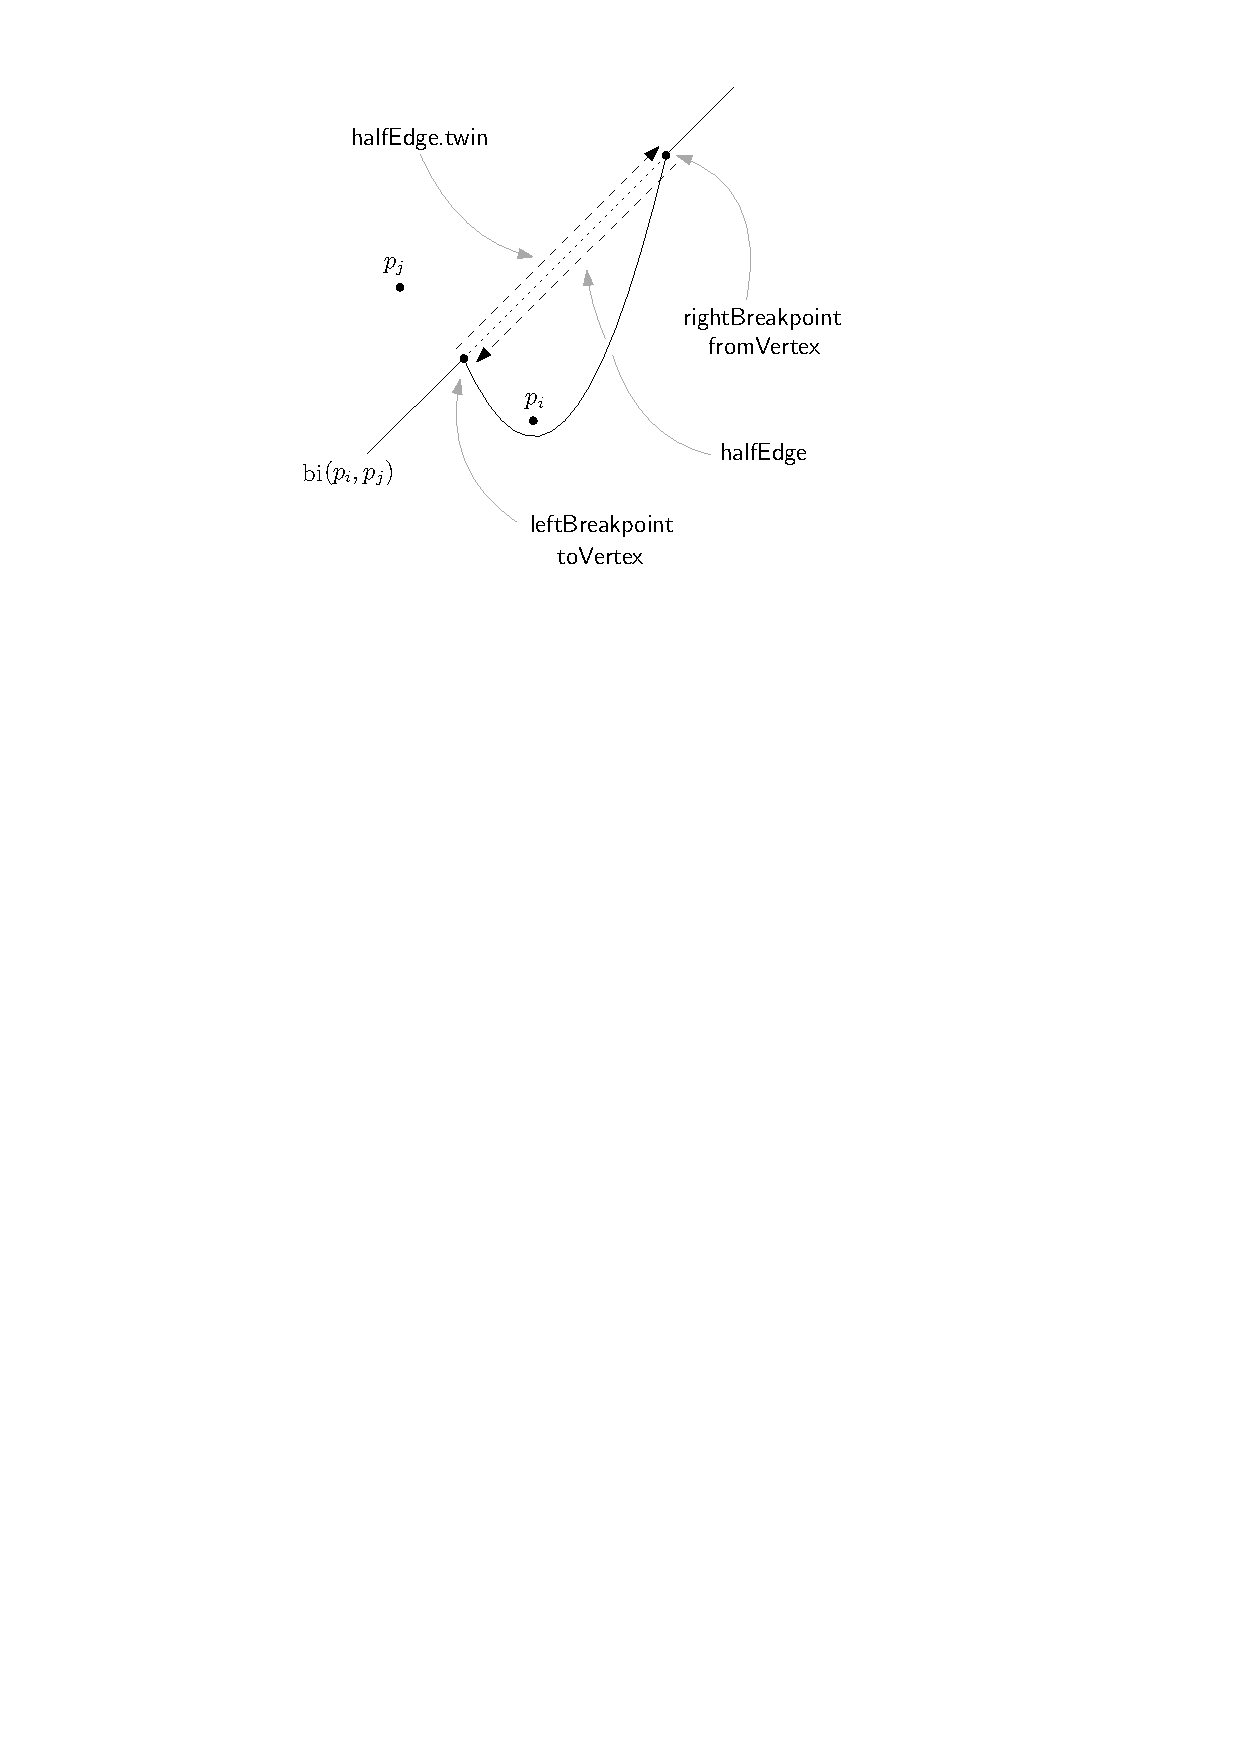
\includegraphics[scale=0.6]{images/dcel_site_event}
\]

\subsection{Updating DCEL at circle event}
\todo{Describe how we modify the DCEL at a circle event}
\[
    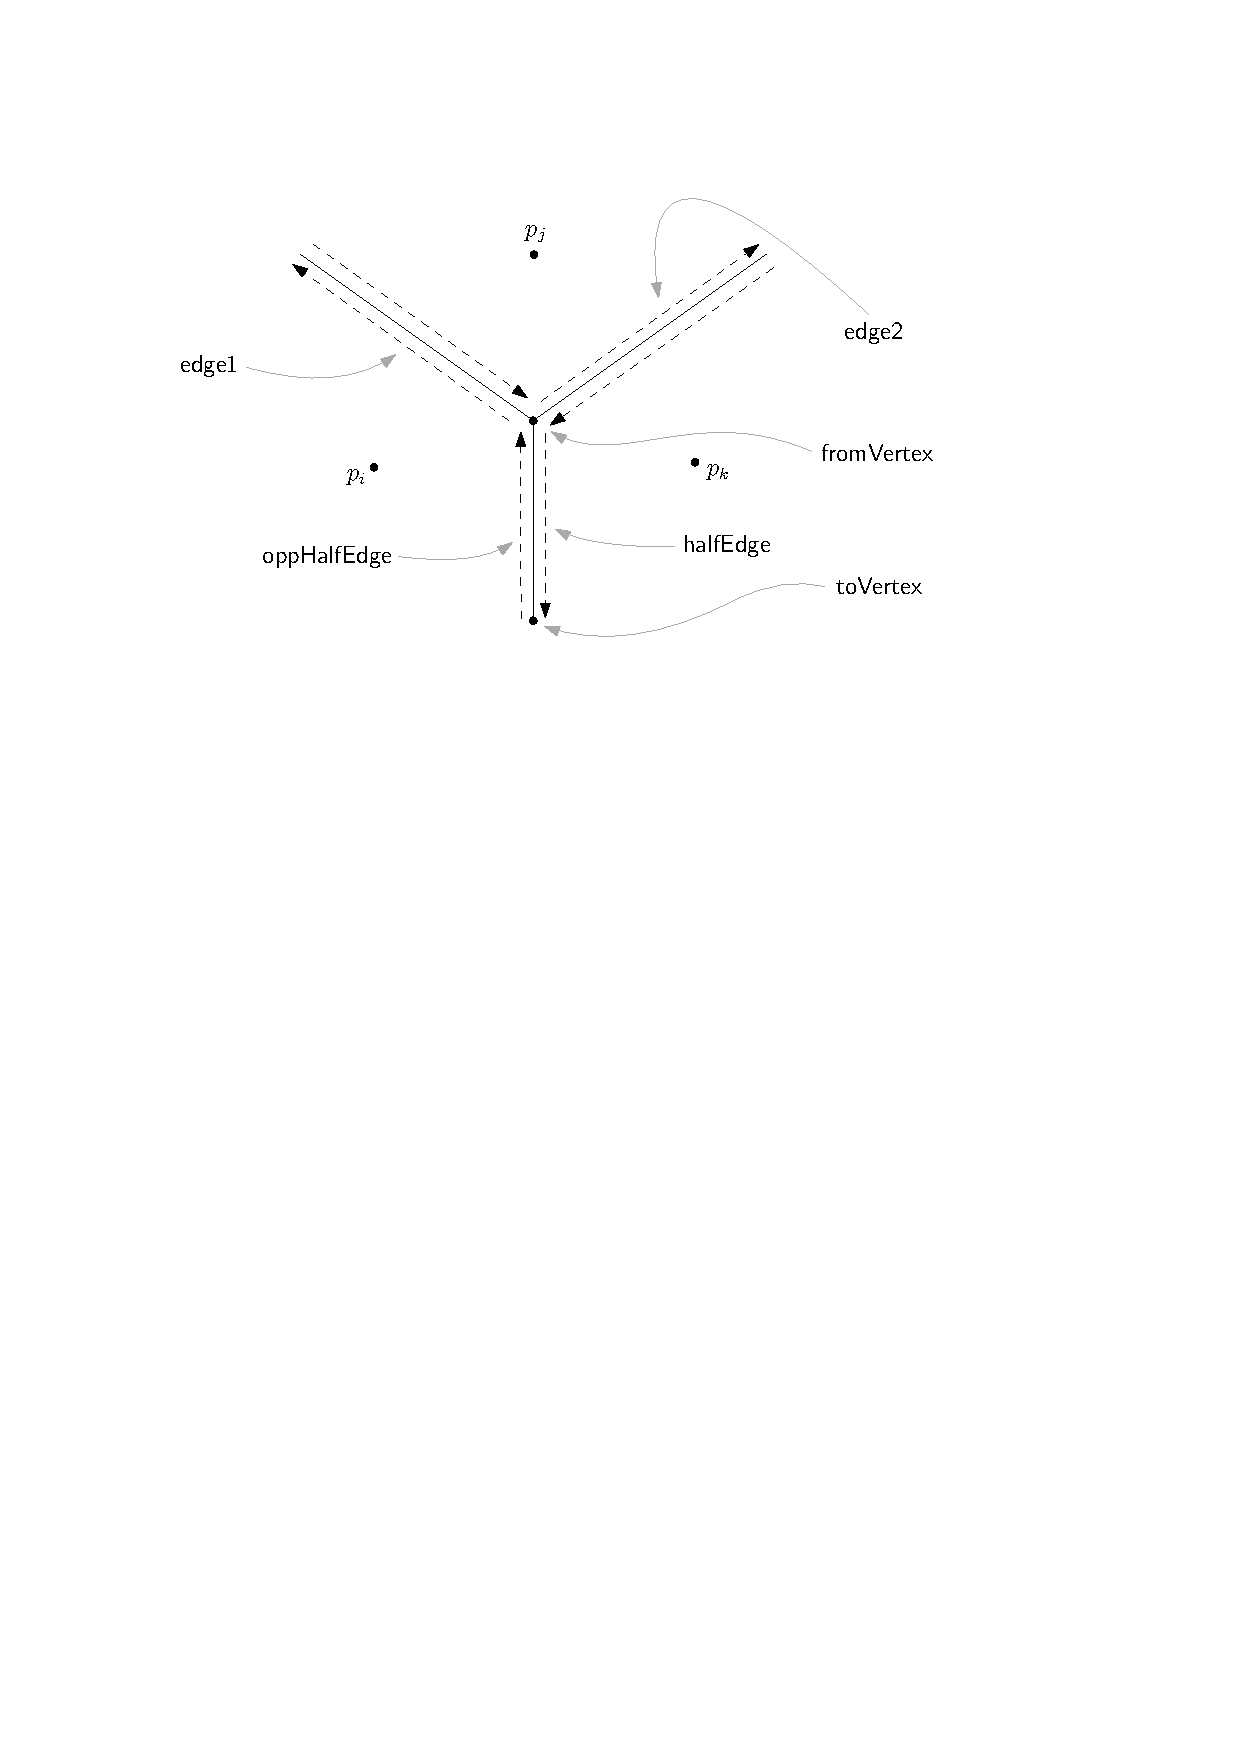
\includegraphics[scale=0.6]{images/dcel_circle_event}
\]

\todo{Describe how we intersect the DCEL with a bounding box when we have been through the event queue}
\chapter{Description of Fortune's algorithm}

We are now ready to describe Fortune's algorithm. We start with describing an overview of the algorithm, and then in the next section we describe some of the details thoroughly -- so anytime the algorithm says ``see detail $n$'', then this detail can be found in the next section.

\begin{alg} \label{alg:fortune} \textsc{VoronoiDiagram}(P) \\
\textit{Input:} A set $P = \curly{p_1, \ldots, p_n}$ of point sites in the plane. \\
\textit{Output:} The Voronoi diagram $\Vor(P)$ given inside a bounding box in a doubly-connected edge list $\mathcal{D}$.
\begin{enumerate}
    \item Initialize the event queue $\mathcal{Q}$ with a site event for every point in $P$, initialize the beach line tree $\mathcal{T}$ to be \textsc{nil}, and let the DCEL $\mathcal{D}$ be empty.
    \item Repeat the following until $\mathcal{Q}$ is empty:
    \begin{enumerate}[i.]
        \item Remove the event $e$ with the largest $y$-coordinate from $\mathcal{Q}$.
        \item If $e$ is a site event call \textsc{HandleSiteEvent}$(e)$.
        \item If $e$ is a site event call \textsc{HandleCircleEvent}$(e)$.
    \end{enumerate}
    \item At this point the internal nodes in $\mathcal{T}$ represent the infinite edges of $\Vor(P)$. Compute a bounding box $B$ which contains all points in $P$, as well as all the vertices of $\Vor(P)$, which are contained in $\mathcal{D}$. Intersect the infinite edges in $\mathcal{T}$ with $B$ and let these intersection points be new vertices in $\mathcal{D}$. Add new edges and pointers to make sure we still have a proper DCEL structure. (See detail \#)
\end{enumerate}
\end{alg}

\begin{proc} \textsc{HandleSiteEvent}$(e)$
\begin{enumerate}
    \item Let $p_i$ denote the site that $e$ points to.
    \item If $\mathcal{T} = \textsc{nil}$ then let $\mathcal{T}$ store the single arc that is described by $p_i$ and return.
    \item Otherwise, $\mathcal{T} \ne \textsc{nil}$. Search in $\mathcal{T}$ for the arc $\alpha$ vertically above $p_i$, that is the arc at which the vertical line through $p_i$ intersects the beach line. (See detail \#)
    \item If $\alpha$ has a pointer to a circle event $e'$, then remove $e'$ from $\mathcal{Q}$, as this circle event is now a false alarm since $\alpha$ is about to disappear earlier than we initially thought.
    \item Create the new arc $\beta$ defined by $p_i$ and insert it into $\mathcal{T}$ as described in Section \ref{sec:insertingatsiteevents}. Update $\mathcal{D}$ by creating the new half-edges which will be traced out by the two new breakpoints as described in Section \ref{sec:dcelatsiteevents}.
    \item Check the triple of consecutive arcs where the new arc for $p_i$ is the left arc to see if the breakpoints converge. If so, insert the circle event into $\mathcal{Q}$ and add pointers between the node in $\mathcal{T}$ and the node in $\mathcal{Q}$. Do the same for the triple where the new arc is the right arc. (See detail \#)
\end{enumerate}
\end{proc}

\begin{proc} \textsc{HandleCircleEvent}$(e)$
\begin{enumerate}
    \item Let $\alpha$ be the arc pointed to by $e$, which is about to disappear from the beach line.
    \item Delete all circle events from $\mathcal{Q}$ which involve $\alpha$: The one where $\alpha$ is the middle arc has already been deleted, and the other two possible circle events where $\alpha$ is the left and right arc respectively can be found through $\alpha$'s \textsf{.leftArc} and \textsf{.rightArc} pointers. (See detail \#)
    \item Delete $\alpha$ from $\mathcal{T}$, how this is done is described in Section \ref{sec:deletingatsiteevents}.
    \item Add the center $c$ of the circle describing $e$ as a new vertex of $\mathcal{D}$. Connect the half-edges in $\mathcal{D}$ that converge at $e$, and create a new half-edge which starts at $c$ and setup the appropriate pointers. The details are given in Section \ref{sec:dcelatcircleevents}.
    \item As $\alpha$ disappears from the beach line, we get new triples of consecutive arcs which might have converging breakpoints that can lead to a circle event. Check these and add circle events if needed. (See detail \#)
\end{enumerate}
\end{proc}

\section{Details}

\subsection*{Detail 1: Intersecting lines, rays and segments}
As a subroutine in several steps during the algorithm we will need to intersect line segments or rays with each other. We start by describing a solution to this in general. This detail assumes that the reader is familiar with basic linear algebra. We want to find the intersection between 2 lines. We parametrize the lines as follows:
\[
    \gamma_1(t) = p + t d_1 \quad \text{and} \quad
    \gamma_2(s) = q + s d_2,
\]
where $p$ and $q$ are points on the lines, and $d_1$ and $d_2$ are direction vectors which tells us which way the lines point. The situation is illustrated as follows:
\[
    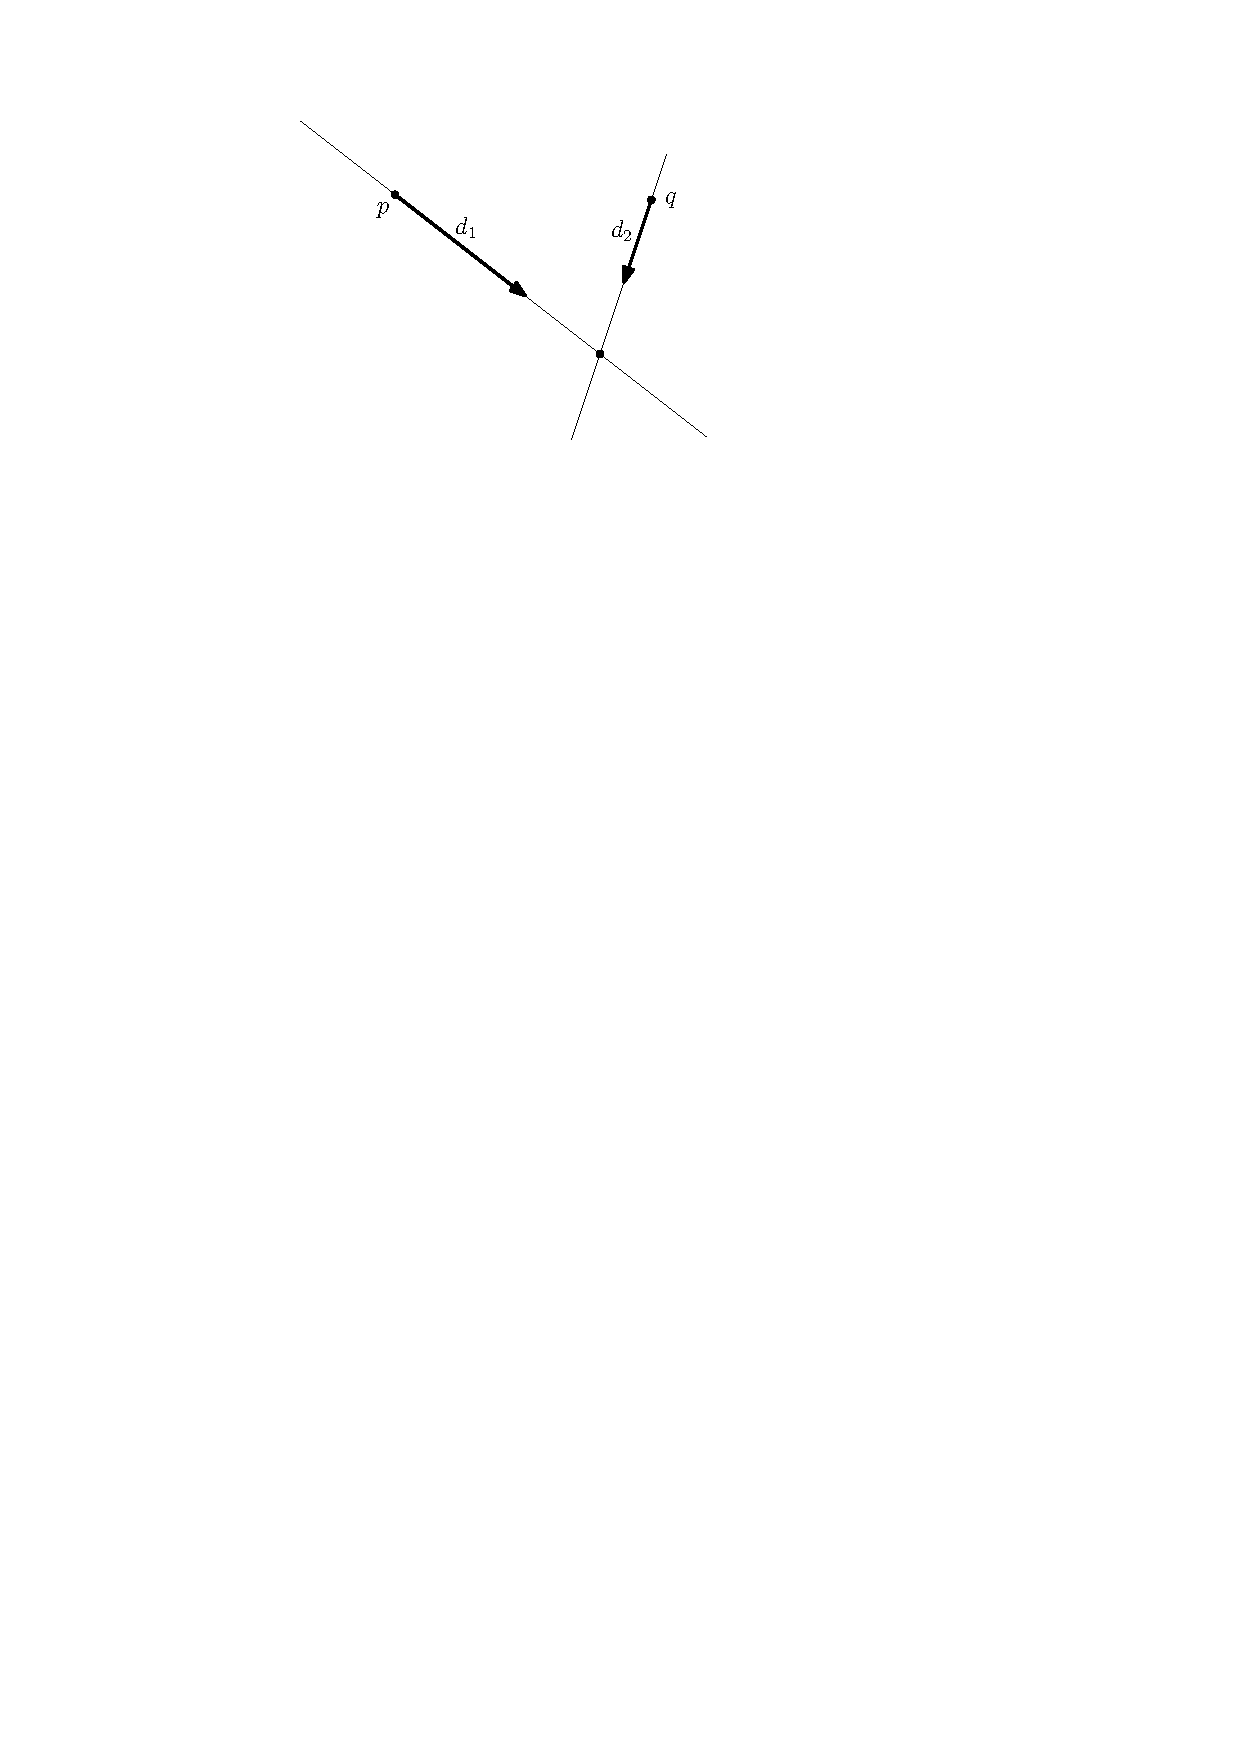
\includegraphics[scale=0.8]{intersect_lines}
\]
To find an intersection point, we must find $s, t \in \R$ such that
\[
    \gamma_1(t) = \gamma_2(s).
\]
That is, we want to solve
\[
    p + t d_1 = q + s d_2.
\]
This can be rewritten into the matrix equation
\[
    A \begin{pmatrix}
        s \\
        -t
    \end{pmatrix}
    =
    q - p,
\]
where $A = \begin{pmatrix} \mid & \mid \\ d_1 & d_2 \\ \mid & \mid \end{pmatrix}$ is the $2 \times 2$ matrix which has $d_1$ and $d_2$ as left and right columns, respectively. The equation system has a unique solution if $d_1$ and $d_2$ are linearly independent, and if they are, the solution is given by
\[
    \begin{pmatrix}
        s \\
        -t
    \end{pmatrix}
    =
    A^{-1} (q - p).
\]
This linear independence property is equivalent to checking that the determinant $\det(A)$ is non-zero. So, in order to check if two lines intersect, we first check if $\det(A) \ne 0$. If not, we say the lines don't intersect. Otherwise, they intersect, and we use the above solution to find the intersection point.

Now in the case of line segments and rays, we also need some constraints on $s$ and $t$, it is not enough that the lines themselves intersect.

To intersect line segments, where the first line segment is given as the points between $p_1$ and $p_2$, and the second line segment is given as the points between $q_1$ and $q_2$, then we let $p = p_1$ and $q = q_1$ and then set $d_1 = p_2 - p_1$ and $d_2 = q_2 - q_1$ and then we solve the equation system as above. If there is a solution to the equation system, then we also need to check that $s \in [0, 1]$ and $t \in [0, 1]$ in order for the intersection point to lie on both of the line segments.

Finally, we look at intersecting two rays. We describe the rays as the lines at the start of this detail, but now we have the requirement that $s, t \geq 0$, which gives us that the rays start at $p$ and $q$, and then they shoot out in the direction of $d_1$ and $d_2$, respectively.

\subsection*{Detail 2: Choose breakpoint based on the ordering of tuple}
Let $p_i$ and $p_j$ be two sites and let $\beta_i$ and $\beta_j$ be the hyperbolas that they describe. If a breakpoint stores the tuple $(p_i, p_j)$ then we want a way to find the $x$ coordinate of that breakpoint. Since the intersection of two hyperbolas may contain 2 intersection points, we need to pick the correct one. We already described this when discussing internal tree nodes at the start of Section \ref{sec:bst}, but let's recap: The order is important since the intersection of the hyperbolas defined by $p_i$ and $p_j$ consists of two points, and the order lets us tell these breakpoints apart. If we consider the beach line as running from the left to the right, then at every breakpoint an arc is leaving, and another is entering it. Thus the tuple $(p_i, p_j)$ tells us that we are interested in the breakpoint at which an arc pointing to $p_i$ leaves, and an arc pointing to $p_j$ is entering the beach line. We will need the following result:

\begin{prop} \label{prop:highschool1}
Let $f(x) = a x^2 + b x + c$ be a polynomial with discriminant $D > 0$ with roots $r_1 < r_2$. Then $r = \tfrac{1}{2}(r_1 + r_2)$ is the only solution to $\displaystyle\frac{df}{dx}(r) = 0$ and the expressions $\displaystyle\frac{df}{dx}(r_1)$ and $\displaystyle\frac{df}{dx}(r_2)$ are non-zero and have opposite signs.
\end{prop}
This fact can be visualized as follows:
\[
    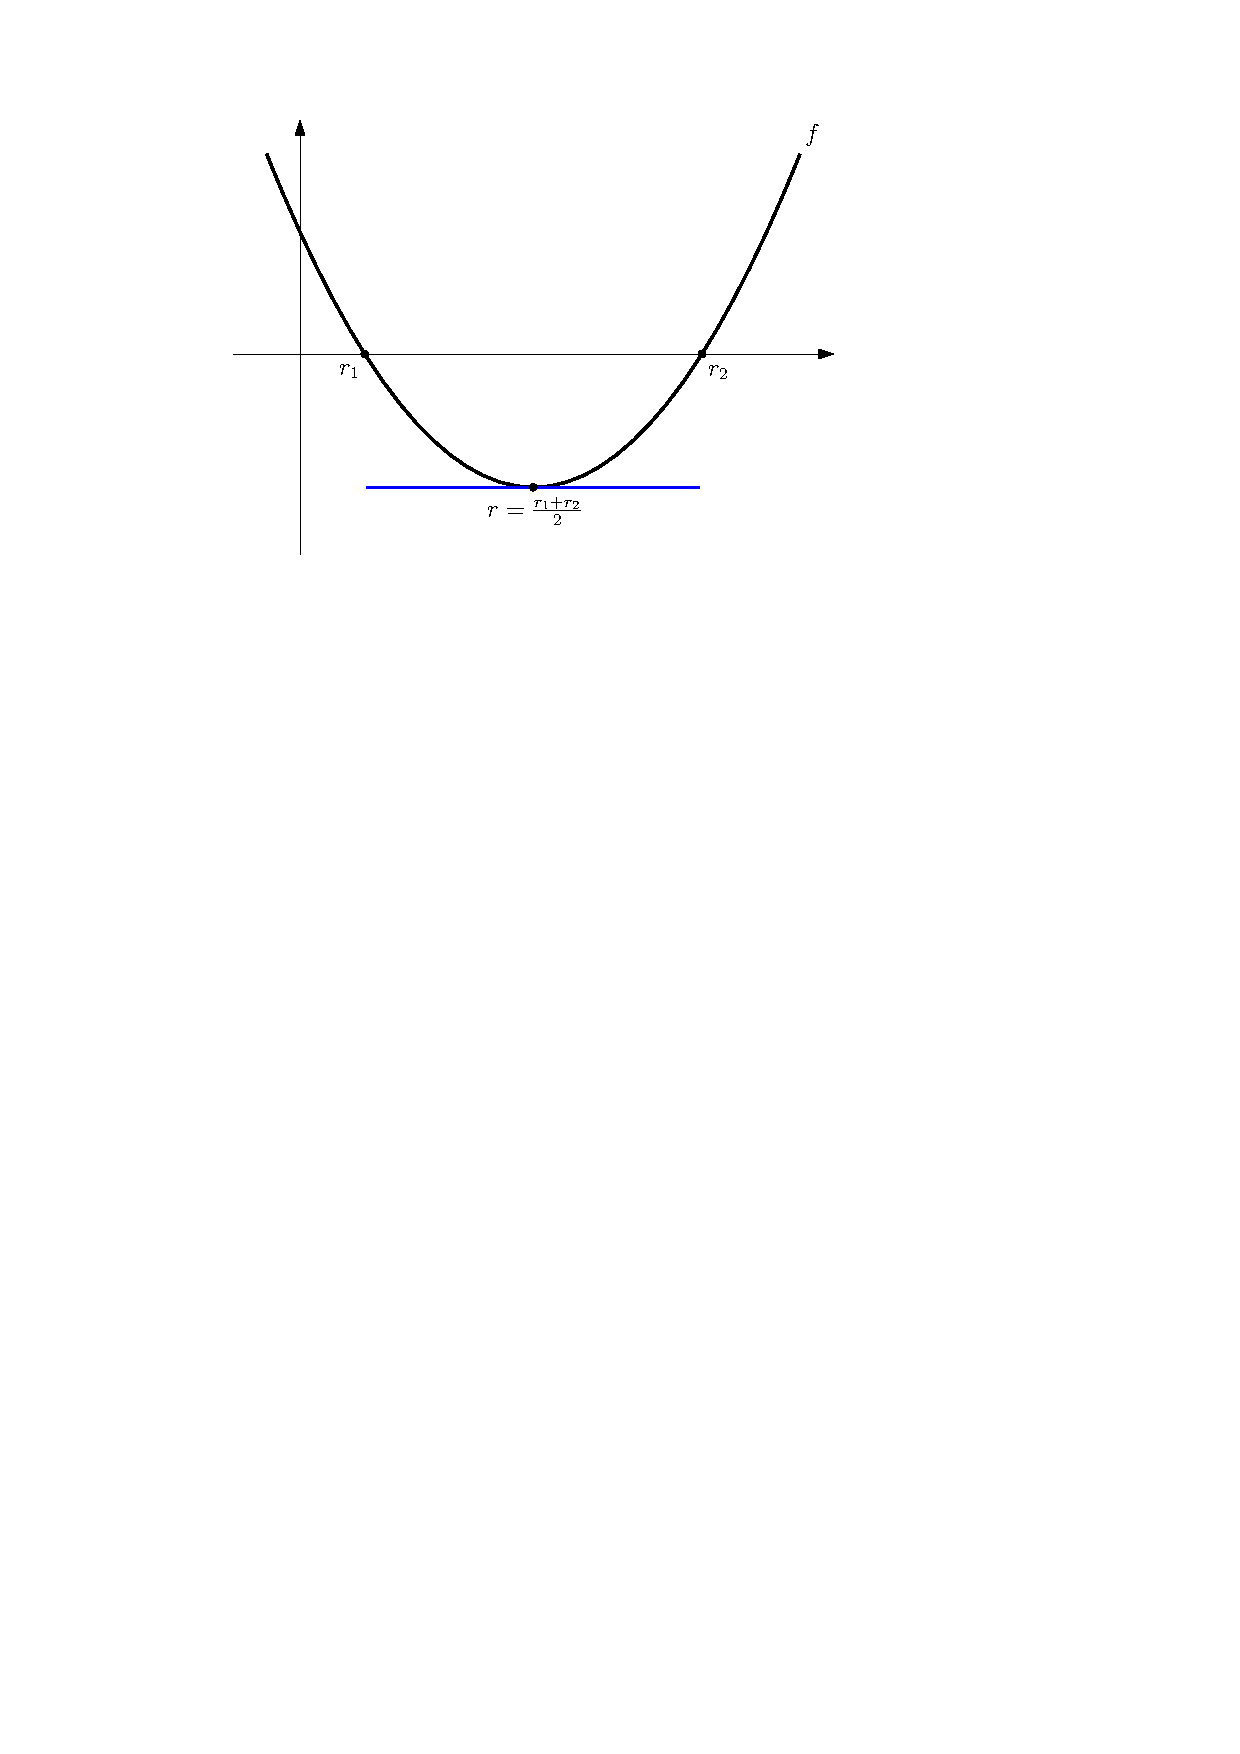
\includegraphics[scale=0.8]{polynomial_result}
\]
\begin{proof}[Proof of Proposition \ref{prop:highschool1}]
It is well-known that we may factor $f$ as follows:
\[
    f = a (x - r_1) (x - r_2) = a x^2 - a(r_1 + r_2) x + a r_1 r_2.
\]
Since two polynomials are equal if and only if their coefficients are equal we get $b = - a (r_1 + r_2)$, which gives us
\[
    \frac{df}{dx} (r) = 2 a r + b = 2 a \para{\frac{r_1 + r_2}{2}} - a (r_1 + r_2) = 0.
\]
This is the only solution since $\displaystyle\frac{df}{dx}$ is a first degree polynomial. Now note that $\displaystyle\frac{d^2 f}{d x^2}(x) = 2a \ne 0$ and $r_1 < r < r_2$ which gives us that
\[
    \text{sgn} \para{\frac{df}{dx}(r_1)} = -\text{sgn} \para{\frac{df}{dx}(r_2)} \ne 0.
\]
\end{proof}
When intersecting two of the paraboals of the beach line, we will find two intersection points, because of our assumptions. Proposition \ref{prop:highschool1} then gives us that at these intersection points $r_1, r_2$ we have that
\[
    \begin{cases}
        \displaystyle\frac{d(\beta_i - \beta_j)}{dx}(r_k) \ne 0 \text{ for } k = 1, 2 & \text{ }\vspace{0.25cm} \\ \text{sgn} \para{\displaystyle\frac{d(\beta_i - \beta_j)}{dx}(r_1)} = -\text{sgn} \para{\displaystyle\frac{d(\beta_i - \beta_j)}{dx}(r_2)} & \text{ }
    \end{cases}
\]
We then want to locate a specific breakpoint between two arcs, and the above will help us to do this.

To intersect the two parabolas $\beta_i$ and $\beta_j$ we write
\[
    (\beta_i - \beta_j)(x) = a x^2 + b x + c,
\]
where (for $p = p_i$, $q = p_j$, $h_p = p_y - \ell_y$ and $h_q = q_y - \ell_y$)
\begin{align*}
    a &= \frac{1}{2} \para{\frac{1}{h_p} - \frac{1}{h_q}}, \\
    b &= \frac{q_x}{h_q} - \frac{p_x}{h_p}, \\
    c &= \frac{q_y(p_x^2 + p_y^2) - p_y (q_x^2 + q_y^2) + \ell_y (q_x^2 + q_y^2 - p_x^2 - p_y^2) + \ell_y^2 (p_y - q_y)}{2 h_p h_q}.
\end{align*}
The square root of the discriminant is then
\[
    d = \sqrt{b^2 - 4 ac} = \sqrt{\frac{(p_x - q_x)^2 + (p_y - q_y)^2}{h_p h_q}}.
\]
The $x$-values of the intersection points are then given by the well-known formulas
\[
    r_1 = \frac{-b - d}{2 a}, \quad
    r_2 = \frac{-b + d}{2 a},
\]
which gives us the intersection points $q_1 = (r_1, \beta_i(r_1))$ and $q_2 = (r_2, \beta_i(r_2))$. Now, we want to find the breakpoint which at which an arc of $\beta_i$ exits the beach line, and an arc of $\beta_j$ enters the beach line. Proposition \ref{prop:highschool1} gives us a way of picking which one of $q_1$ and $q_2$ is the breakpoint that we need. For $\beta_i$ to exit and $\beta_j$ to enter, we need to pick $k$ such that
\[
    \frac{d \beta_i}{dx}(r_k) > \frac{d \beta_j}{dx}(r_k).
\]
This is illustrated in the following figure, with a slight abuse of notation:
\[
    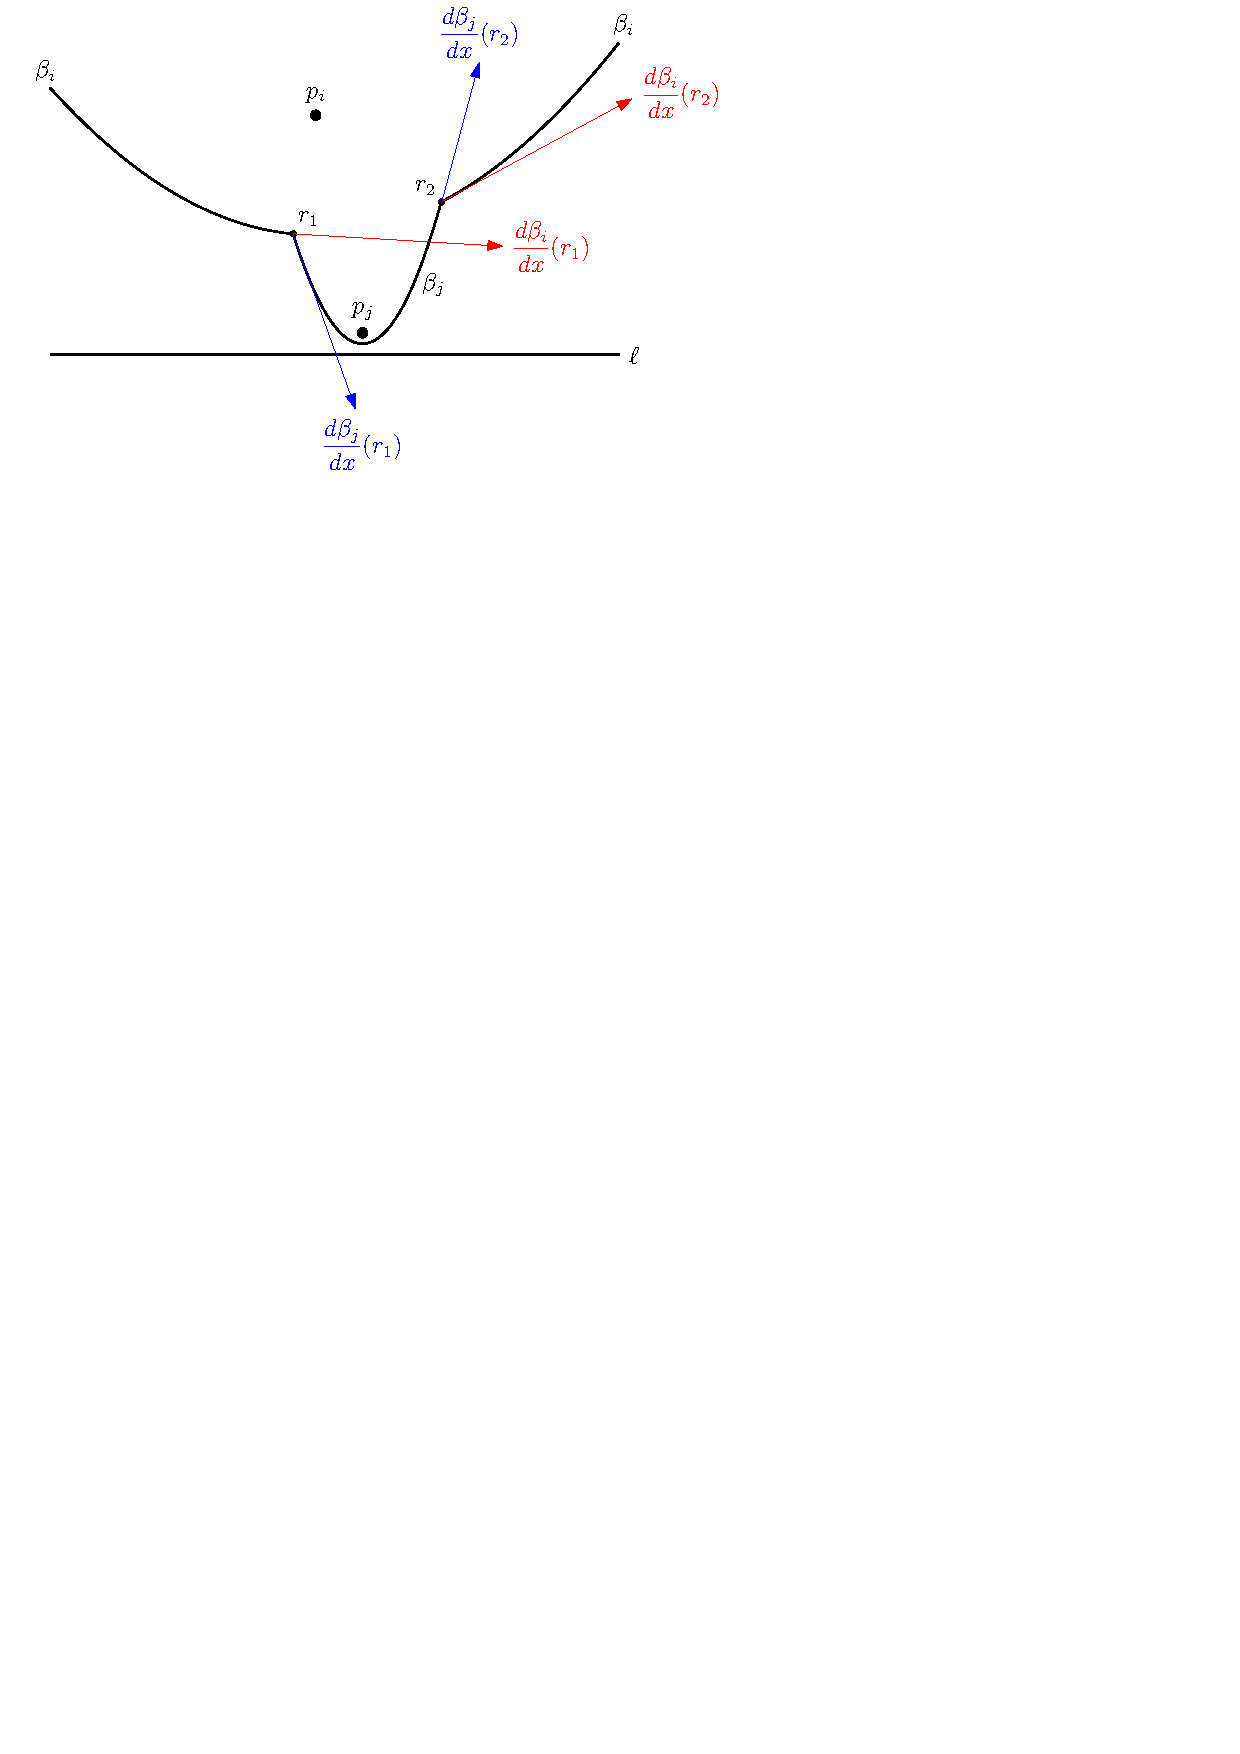
\includegraphics[scale=0.8]{derivativedirections}
\]
Proposition \ref{prop:highschool1} guarantees that either
\begin{align*}
    \frac{d \beta_i}{dx}(r_1) > \frac{d \beta_j}{dx}(r_1) &\text{ and } \frac{d \beta_i}{dx}(r_2) < \frac{d \beta_j}{dx}(r_2) \\
    &\text{or} \\
    \frac{d \beta_i}{dx}(r_1) < \frac{d \beta_j}{dx}(r_1) &\text{ and } \frac{d \beta_i}{dx}(r_2) > \frac{d \beta_j}{dx}(r_2),
\end{align*}
so it is possible to make the right choice. Now, note that by some simple algebraic manipulations we have that
\[
    \frac{d \beta_i}{dx}(r_k) > \frac{d \beta_j}{dx}(r_k)
\]
if and only if
\[
    (r_k - p_x) (q_y - \ell_y) > (r_k - q_x) (p_y - \ell_y).
\]
This gives us a criterion for deciding which intersection point describes the breakpoint in question, and this is the criterion used in the implementation.

\subsection*{Detail 3: How to find the arc vertically above a point}
At a site event when we discover a new point $p$ we want to find the arc $\alpha$ vertically above $p$, as illustrated here:
\[
    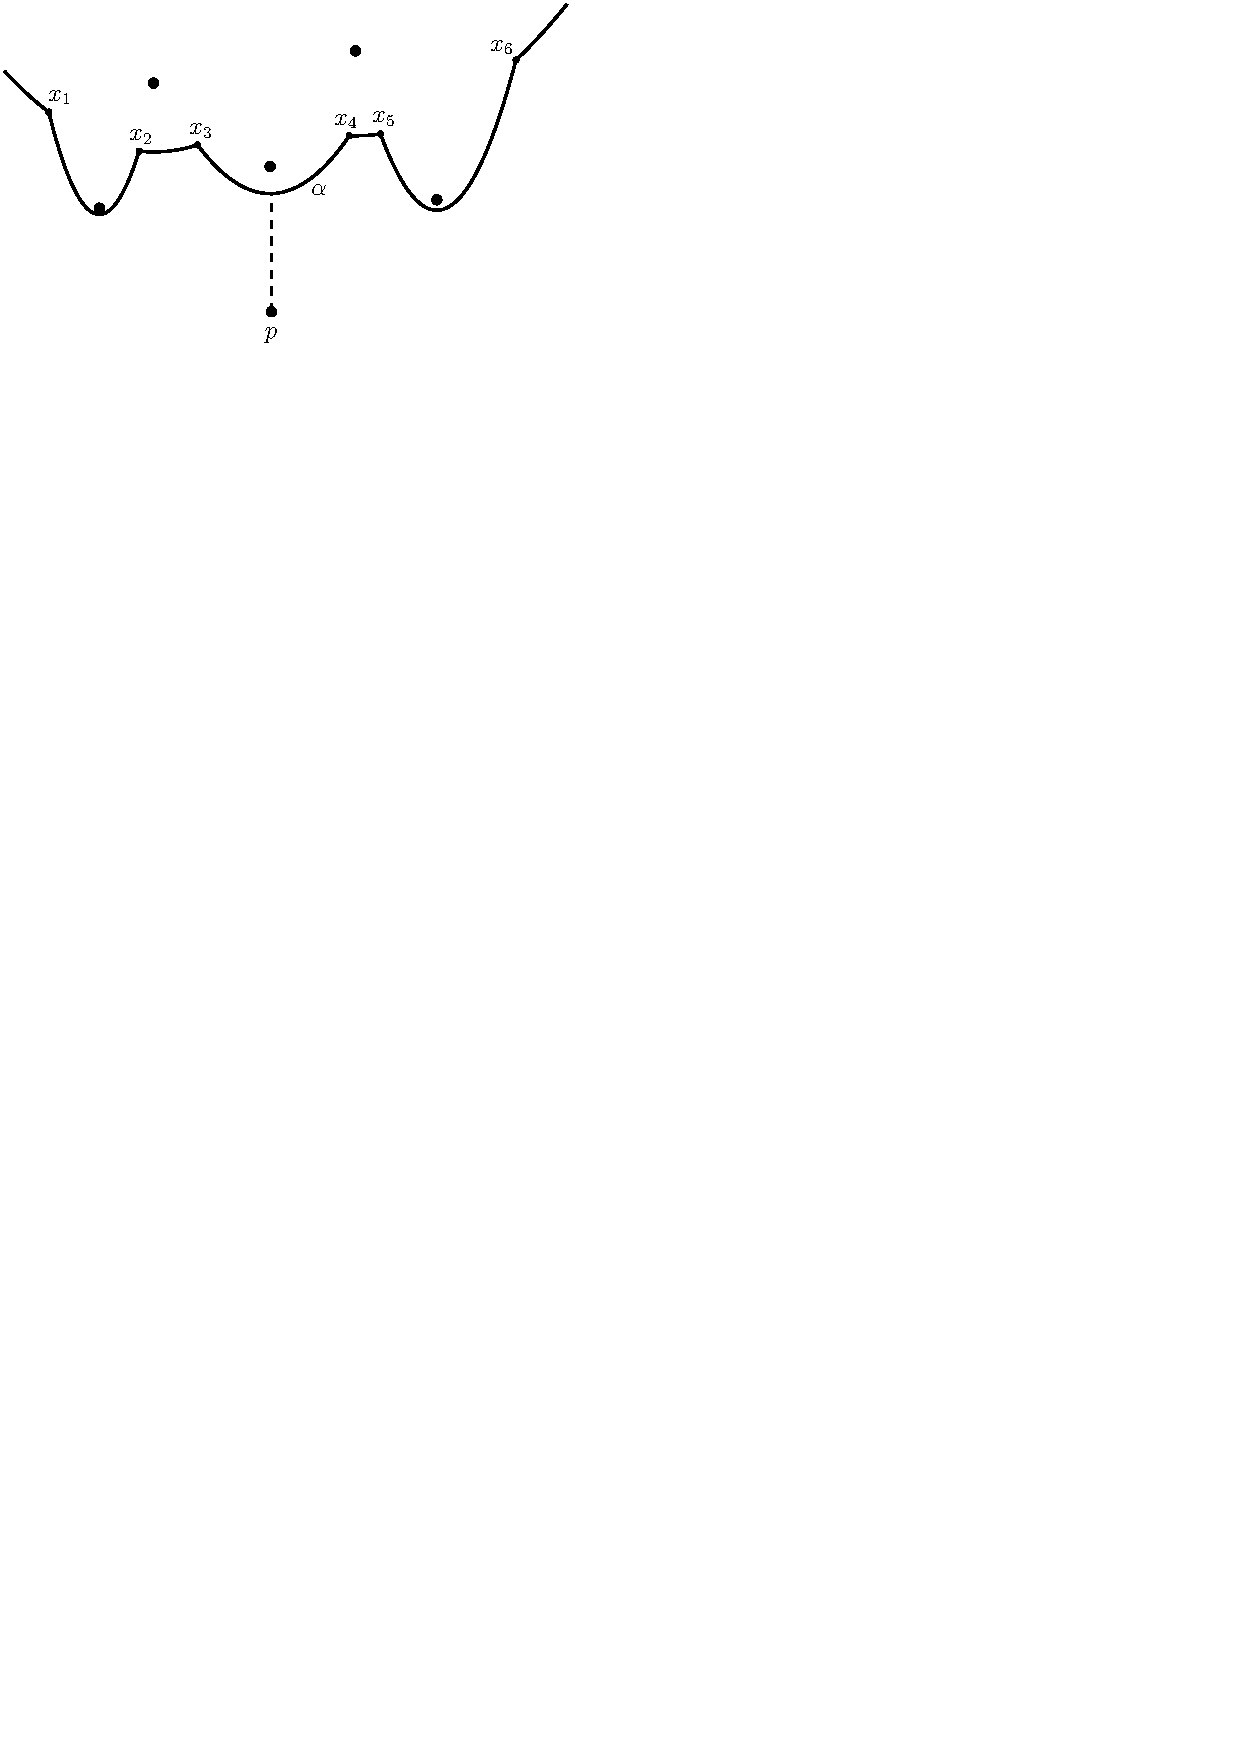
\includegraphics[scale=0.8]{locate_arc}
\]
Let $x_1, x_2, \ldots, x_k$ denote the breakpoints on the beach line. These are stored as internal nodes in our BST $\mathcal{T}$. Since the keys for the internal nodes are the $x$-values of the breakpoints, we may locate the arc $\alpha$ using binary search in $\mathcal{T}$. Starting at an internal node $x$ in $\mathcal{T}$ we visit its left subtree if $x\textsf{.key} < p_x$, and we visit its right subtree if $x\textsf{.key} \geq p_x$. The key property is computed at every check, since it is a function of the current position of the sweep line, see Detail 2 for how the key is computed. Eventually we will reach the leaf which stores the arc $\alpha$.

\subsection*{Detail 4: How to check if two breakpoints are converging}
Let $p, q, r$ be three sites from $P$ which define 3 consecutive arcs on the beach line. Let $x$ and $y$ be two breakpoints, where $x$ is sliding along $\bi(p, q)$ and $y$ is sliding along $\bi(q, r)$ as we vary $\ell$. We want to check whether $x$ and $y$ converge, and if so, what is the location of their intersection, and when during the sweep of $\ell$ will this occur. The two possible scenarios are illustrated below:
\begin{figure}[H]
    \centering
    \subfloat{
      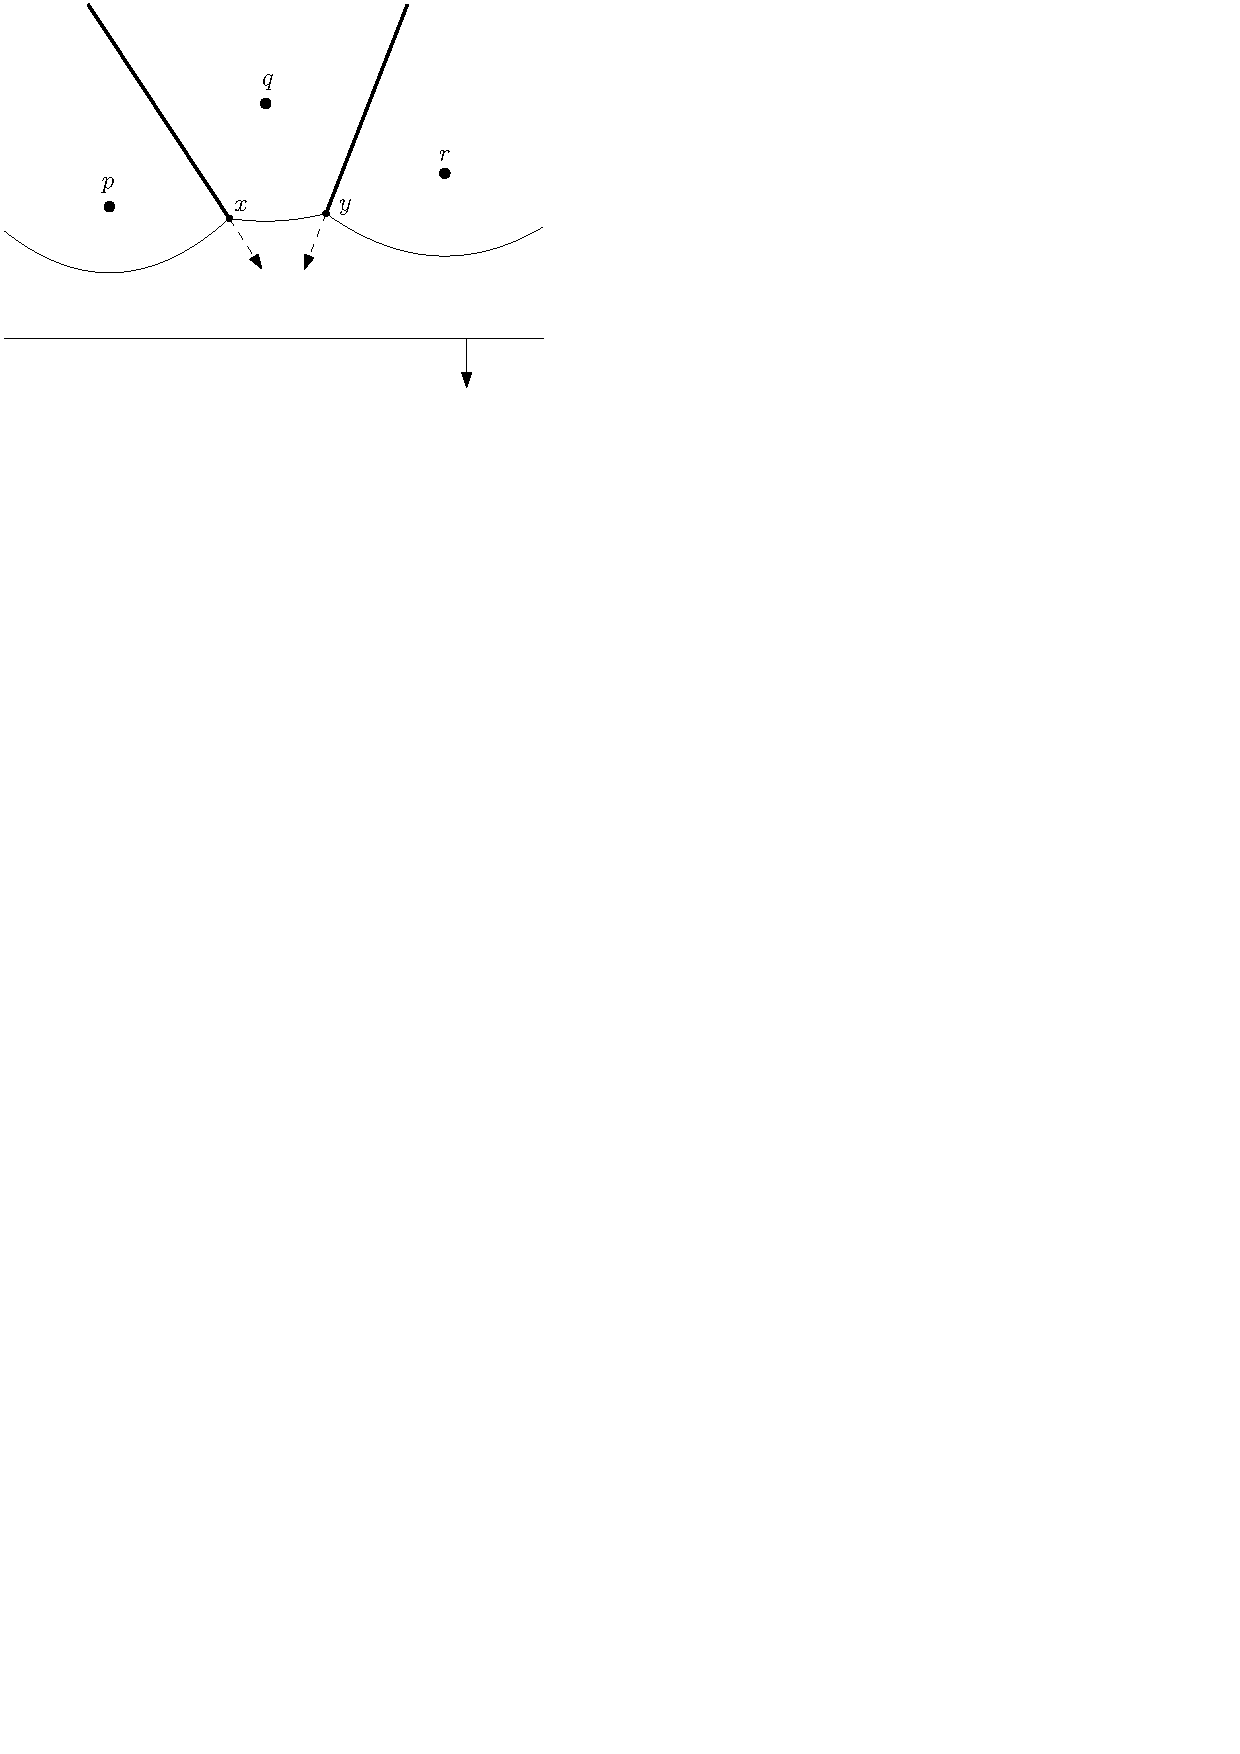
\includegraphics[scale=0.6]{converging_breakpoints_example}
    }
    \subfloat{
      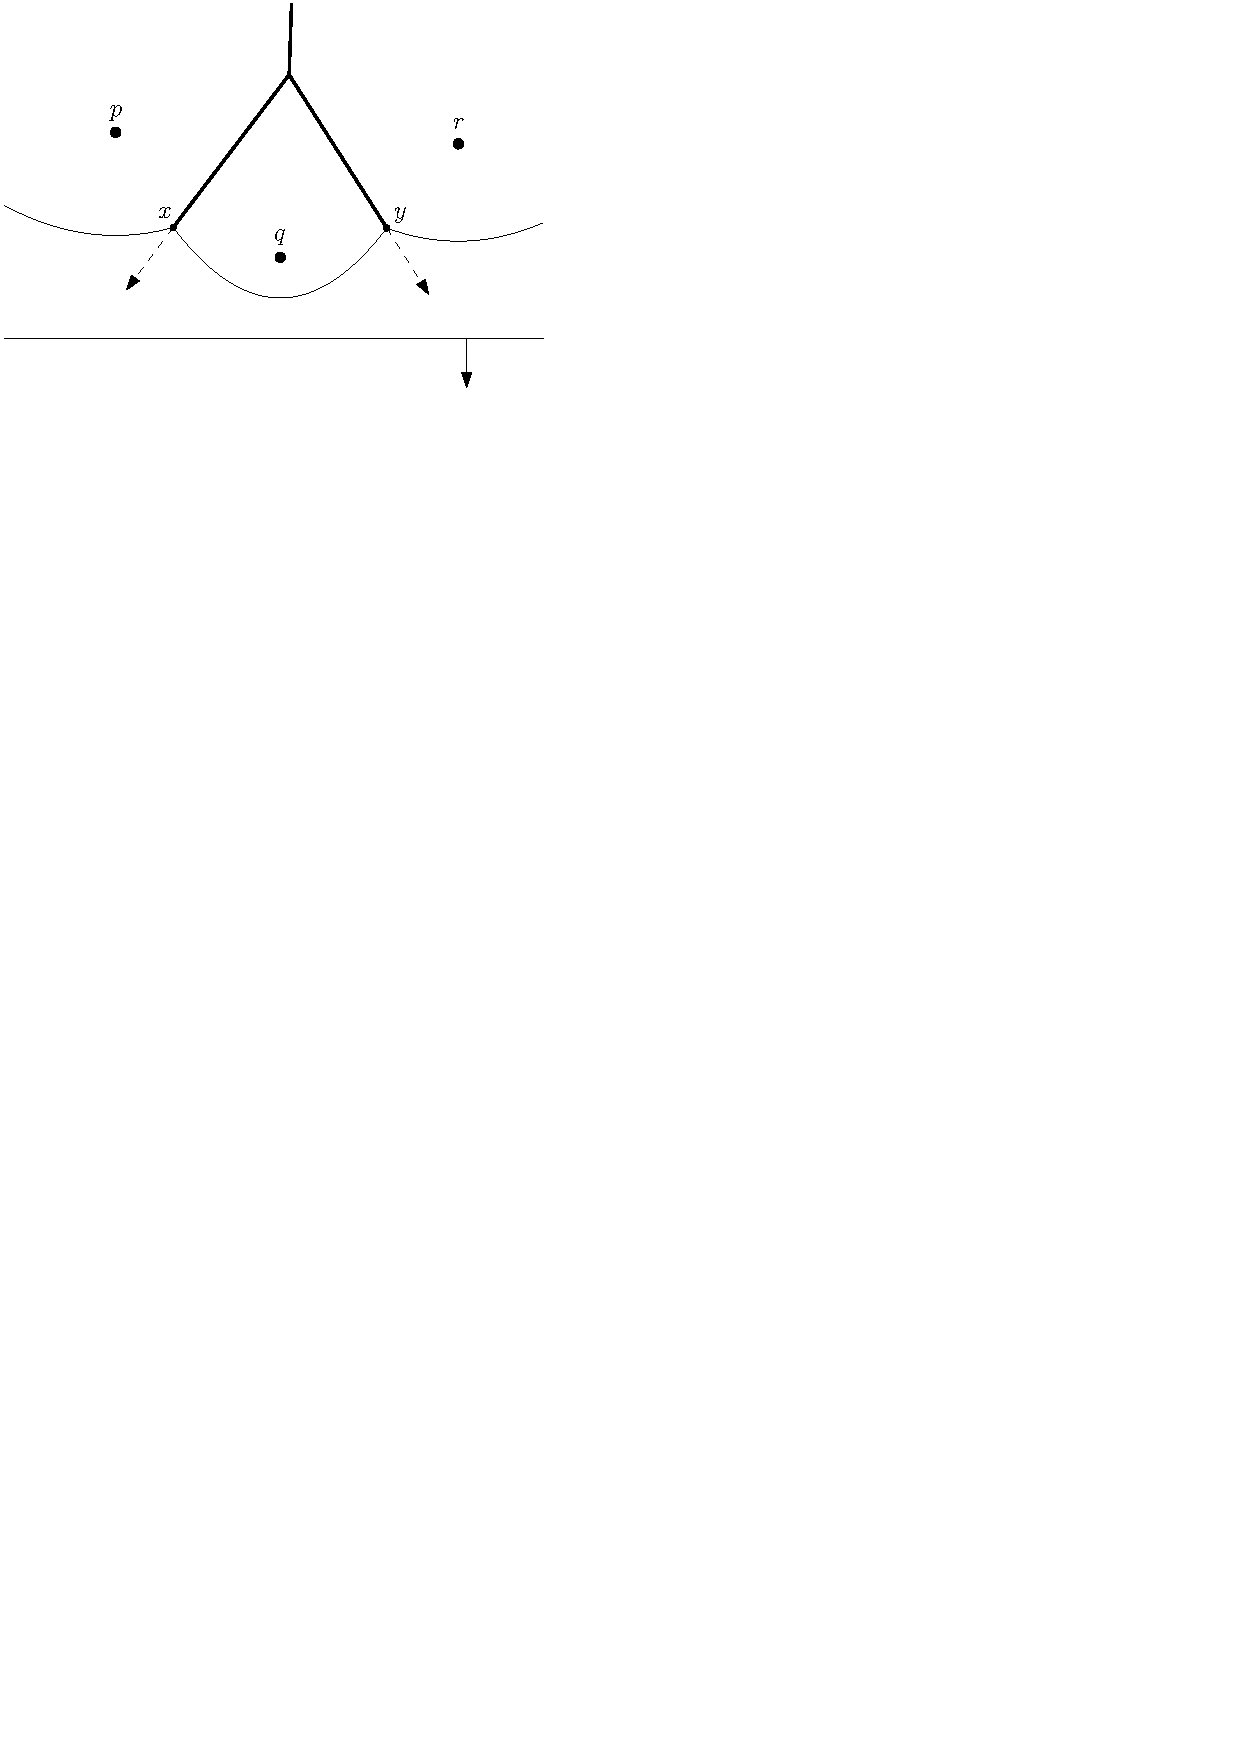
\includegraphics[scale=0.6]{converging_breakpoints_nonexample}
    }
\end{figure}
In the divergent case we include the case where the bisectors are collinear. 

To check for convergence, we transform the problem into a problem of intersecting two rays. Let $x$ and $y$ denote the current location of the breakpoints, and let $x'$ and $y'$ denote the breakpoints new positions after moving the sweep line some arbitrary amount downwards, and then let $d_1 = x' - x$ and $d_2 = y' - y$. Then $s \mapsto x + s d_1$ and $t \mapsto y + t d_2$ parametrize $\bi(p, q)$ and $\bi(q, r)$, respectively. The setup, in the case where the rays do intersect, looks like this:
\[
    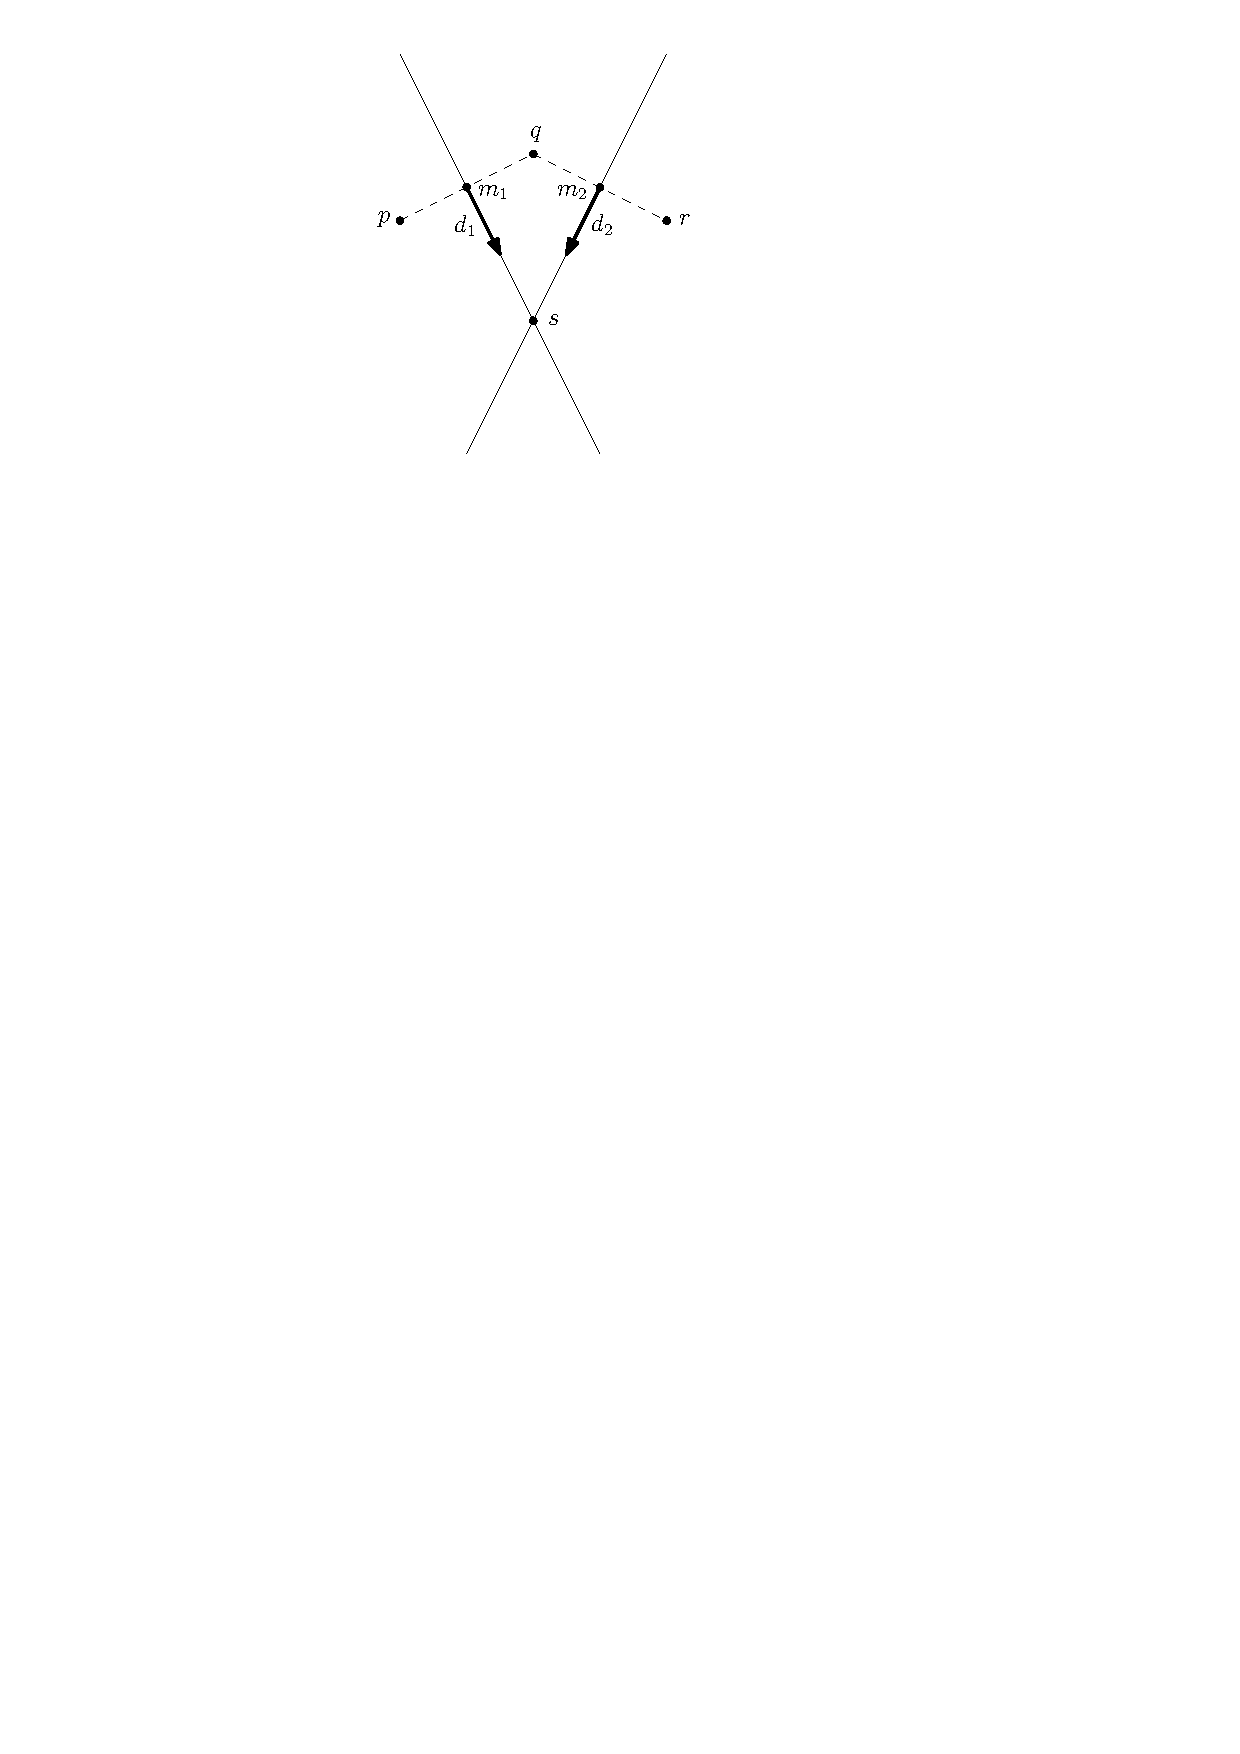
\includegraphics[scale=0.8]{ray_intersection}
\]
Now, as we saw in Detail 1, then the two rays converge if $t \geq 0$ and $s \geq 0$.

This can be interpreted as follows: If $s$ is positive, then that means that $x$ will hit $y$ in the future, and likewise if $t$ is positive, then $y$ will hit $x$ in the future. This is important as we are treating the events chronologically, and if $x$ and $y$ already intersected in the past (or the lines they describe, rather) then they can define no future circle event.

\subsection*{Detail 5: Finding a circle through 3 points}
As a part of the algorithm, we need to find the circle $C$ through 3 points $p, q, r$. It turns out if we intersect $\bi(p, q)$ and $\bi(q, r)$ we find the center of $C$, and then to find the radius we just need to find the distance from the center to one of the points. This is because if $x \in \bi(p, q) \cap \bi(q, r)$ then
\[
    \dist(x, p) = \dist(x, q) = \dist(x, r),
\]
so $x$ is exactly the center of a circle through $p, q, r$. This is illustrated in this figure:
\[
    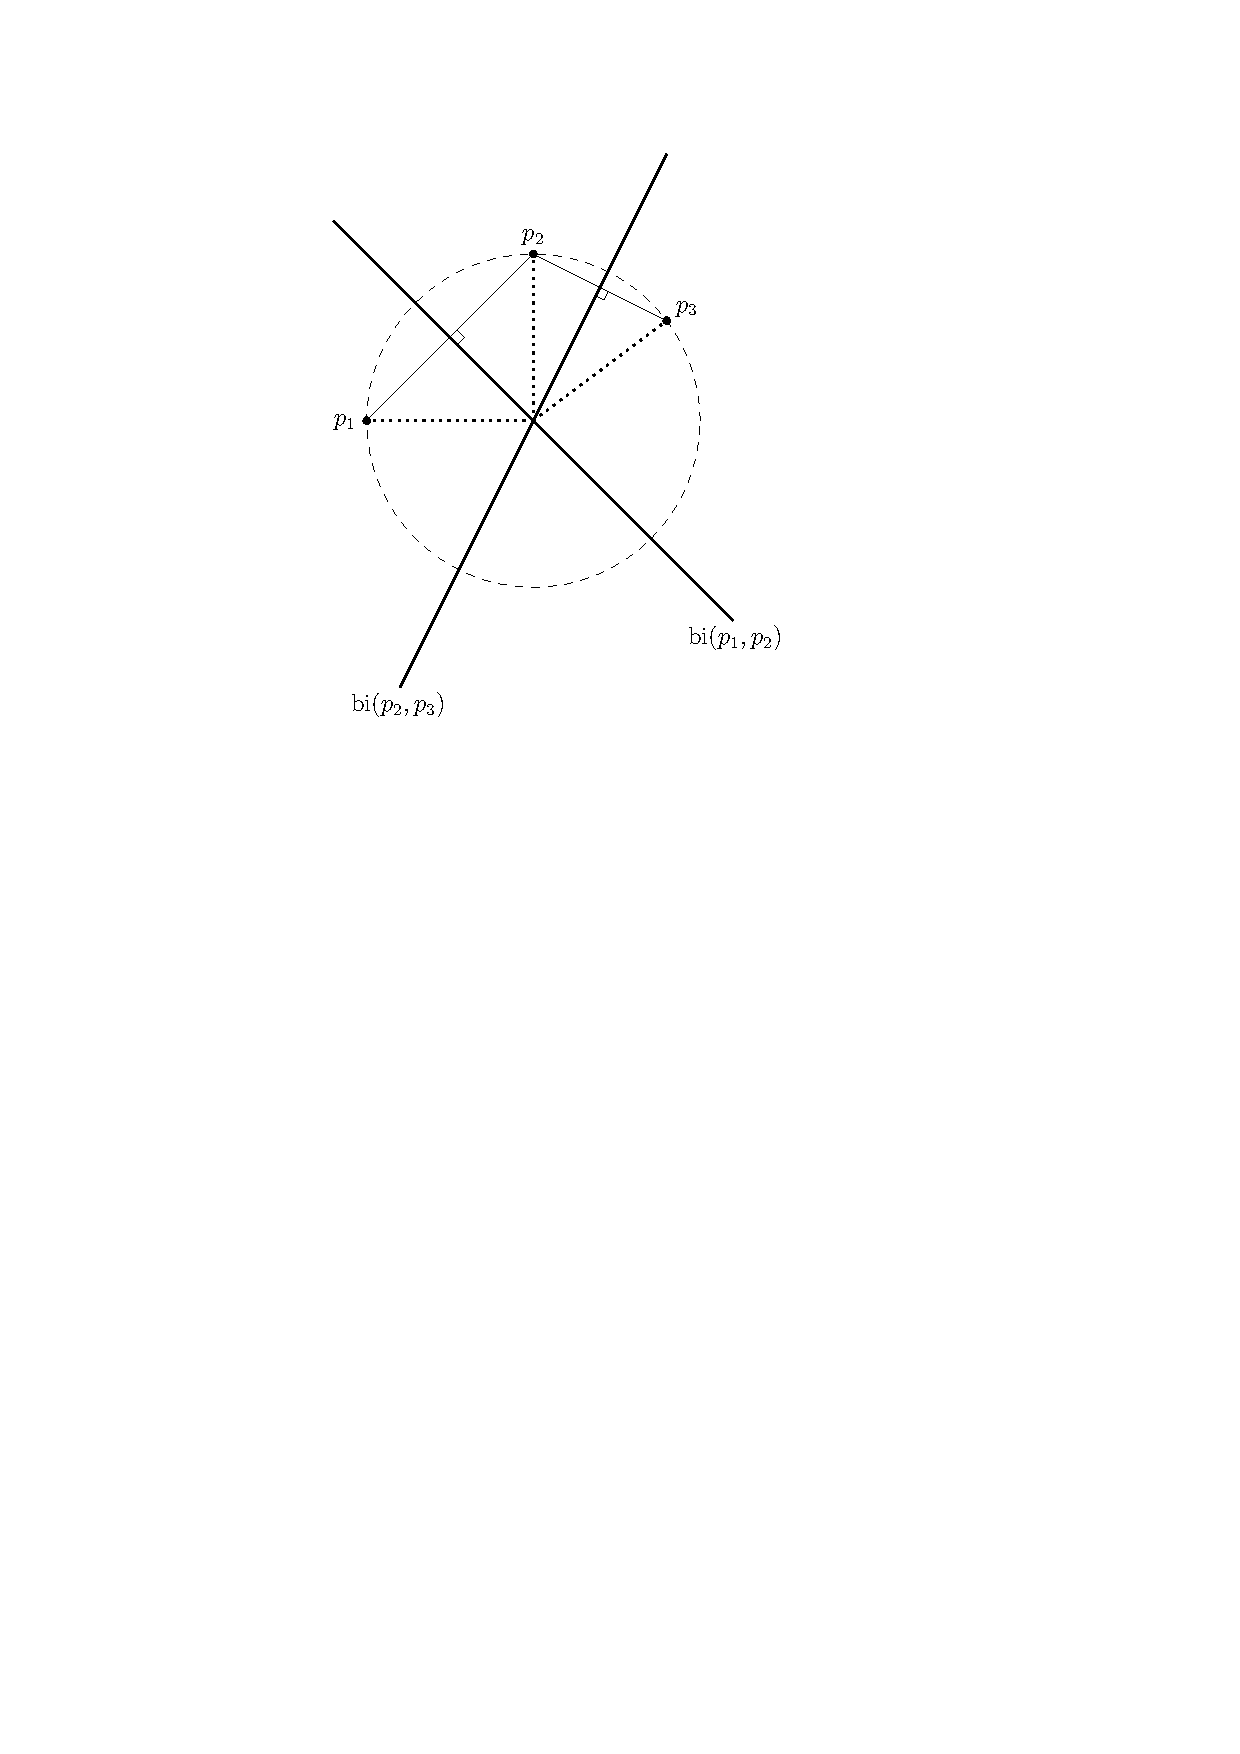
\includegraphics[scale=0.8]{circle_3_points}
\]
To intersect the bisectors, we form the midpoints
\[
    m_1 = \frac{1}{2}(p + q) \quad \text{and} \quad m_2 = \frac{1}{2}(q + r)
\]
and then we let $d_1$ and $d_2$ denote $q - p$ and $r - q$ rotated 90 degrees counterclockwise. Then $s \mapsto m_1 + s d_1$ and $t \mapsto m_2 + t d_2$ parametrize $\bi(p, q)$ and $\bi(q, r)$, respectively. Then we solve the linear system as in Detail 1.

\subsection*{Detail 6: Deleting false alarms during a circle event}
At a circle event an arc disappears from the beach line, along with two breakpoints. Consider the following example, where at one point in time we have the arcs $\alpha_1, \alpha_2, \ldots, \alpha_7$ on the beach line along with the breakpoints $x$ and $y$ that $\alpha_5$ lies inbetween, and then after a circle event the arc $\alpha_5$ disappears after the breakpoints $x$ and $y$ intersect and get replaced by a new breakpoint $z$:
\[
    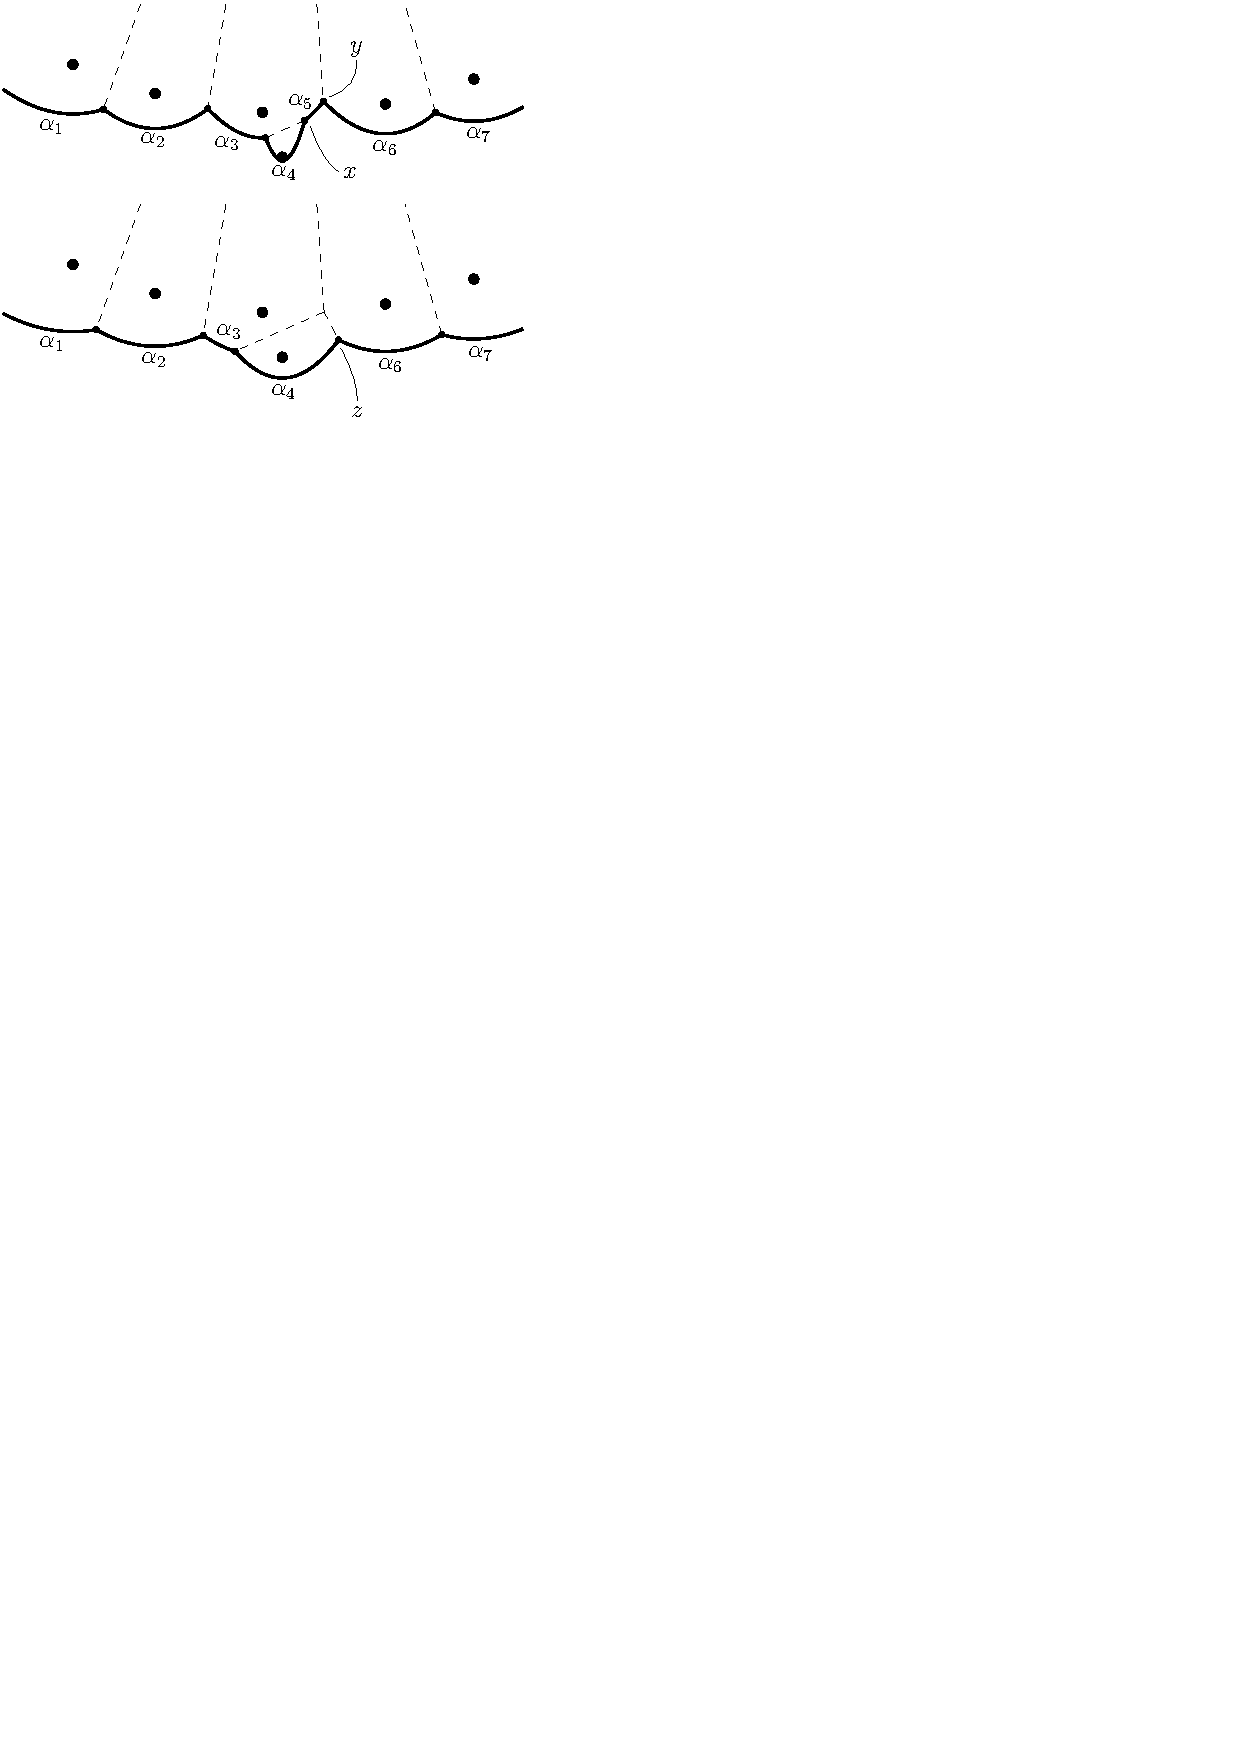
\includegraphics[scale=0.8]{circle_event_beachline_merge}
\]
When this happens, we have to remove the circle events that involve the breakpoints $x$ and $y$ merging with any other breakpoints. Since we set up a linked list of arcs, we can find the arcs $\alpha_4$ and $\alpha_6$ through the \textsf{.leftArc} and \textsf{.rightArc} pointers that $\alpha_5$ has, and if these arcs point to a circle event, then we remove those circle events from $\mathcal{Q}$ if they exist. These are of course found before deleting $\alpha_5$. This covers removing the false alarms, since we have removed circle events from every arc that surrounds $x$ and $y$. This example is general enough to explain the general case.

\subsection*{Detail 7: Checking consecutive arcs for circle events}
First we consider the case of a site event. Assume the beach line is made out of the arcs $\alpha, \beta, \gamma, \delta$ and $\varepsilon$, and assume that $\gamma$ is the new arc we just created. Just a moment later the beach line looks something like this:
\[
    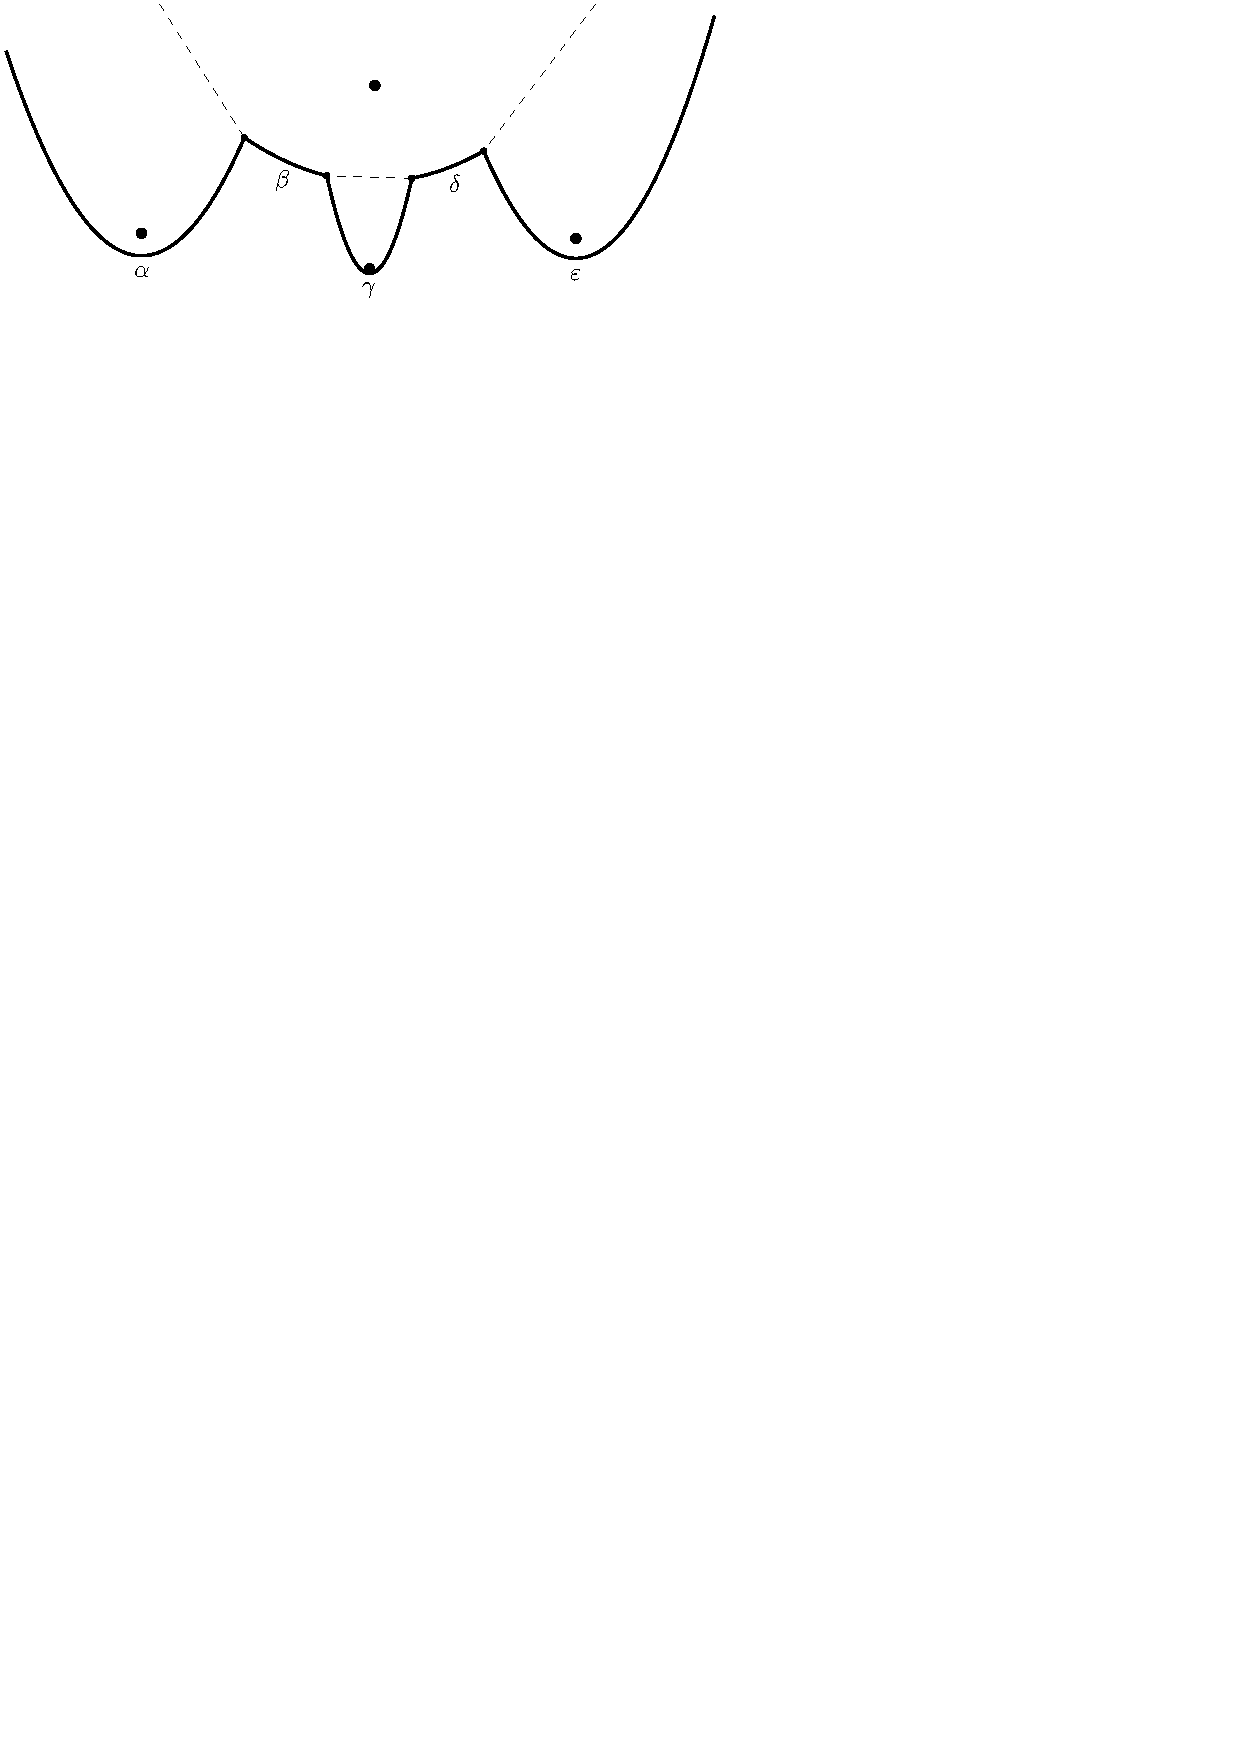
\includegraphics[scale=0.8]{cons_arcs_site_event}
\]
The arcs we need to check for converging breakpoints are then $(\alpha, \beta, \gamma)$ and $(\gamma, \delta, \varepsilon)$. To be more precise, if $p_{\alpha}, p_{\beta}, p_{\gamma}, p_{\delta}$ and $p_{\varepsilon}$ denote the associated sites, then we need to check the convergence of the breakpoints defined by $(p_{\alpha}, p_{\beta})$ and $(p_{\beta}, p_{\gamma})$, and to check the convergence of the breakpoints defined by $(p_{\gamma}, p_{\delta})$ and $(p_{\delta}, p_{\varepsilon})$, and in case of convergence we must add circle events.

Now we consider the case of a circle event. Assume the beach line just before the circle event contained the consecutive arcs $\alpha, \beta, \gamma, \delta$ and $\varepsilon$. At the circle event the arc $\gamma$ then disappears, now connecting $\beta$ and $\delta$, leaving us with the following picture:
\[
    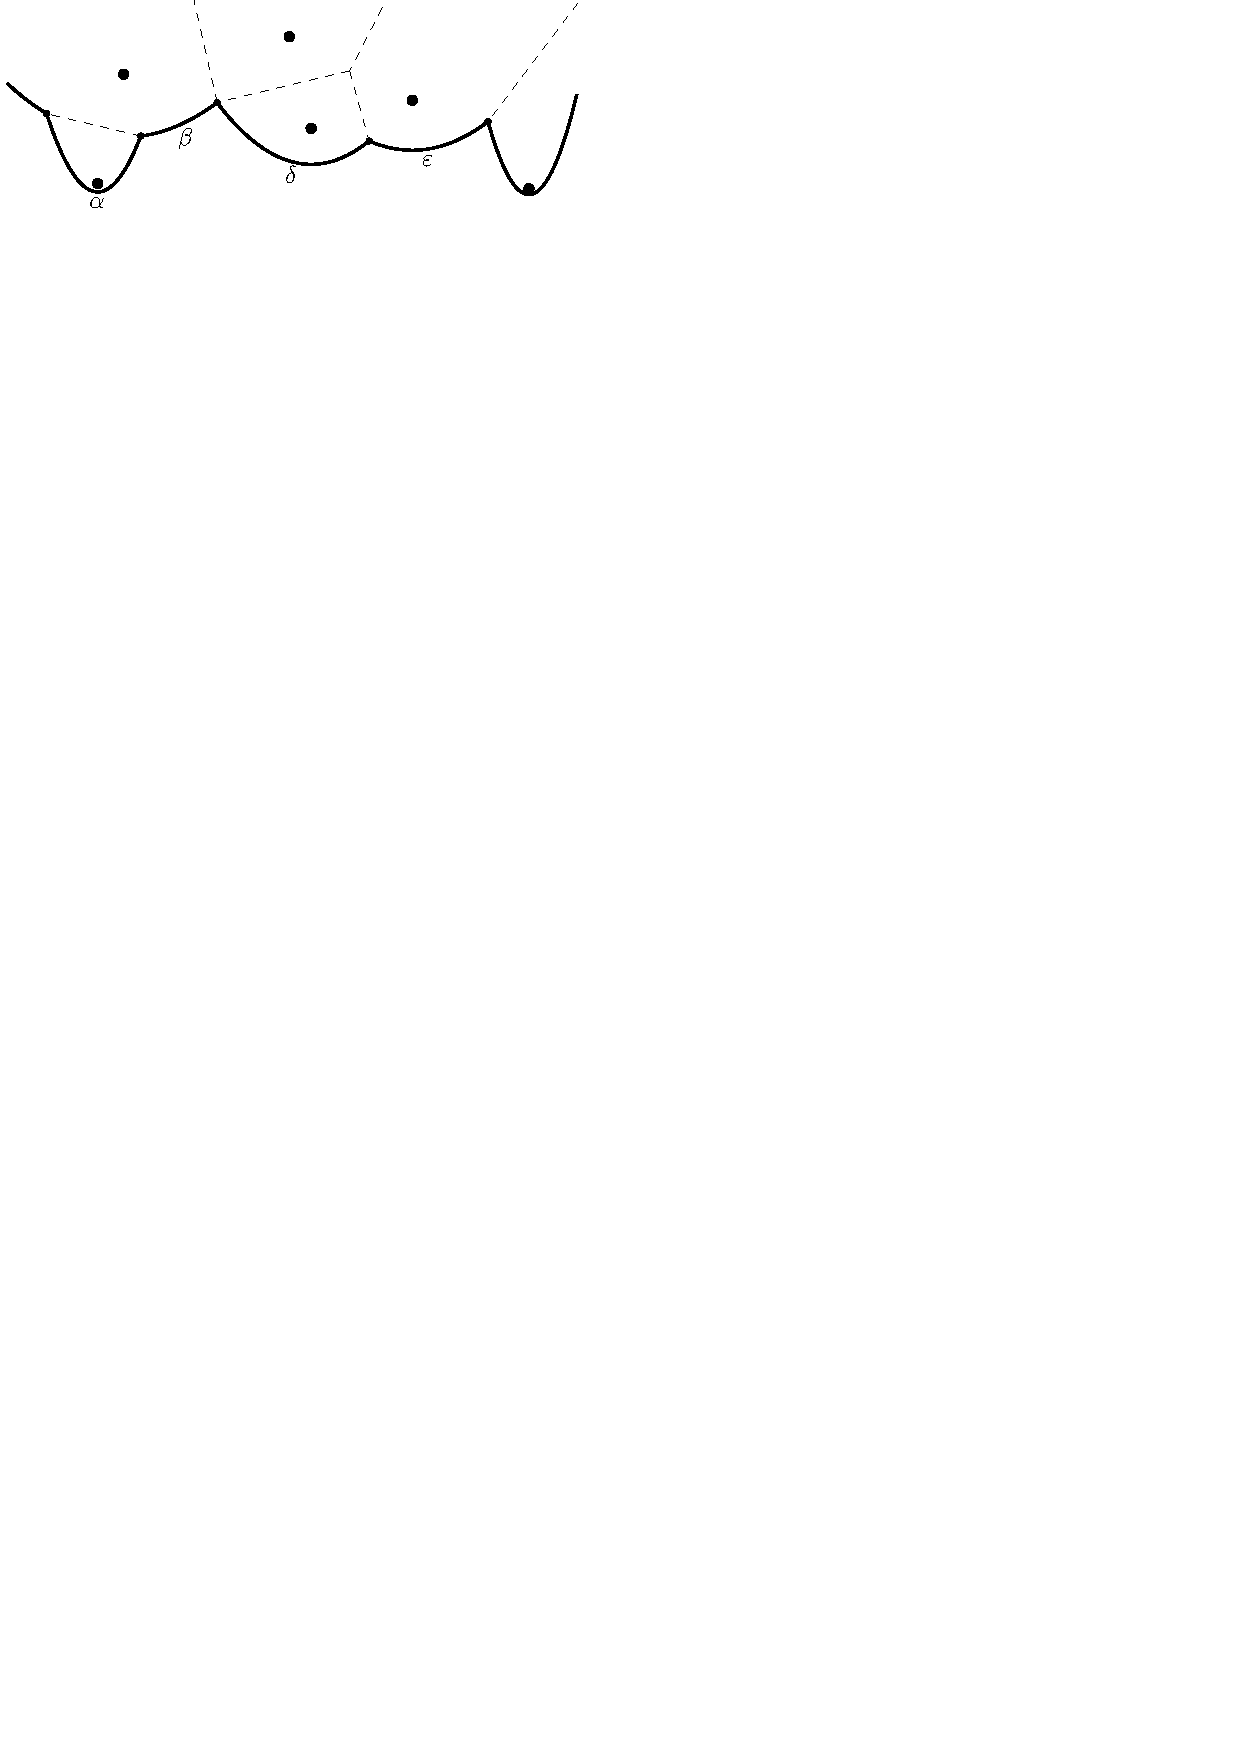
\includegraphics[scale=0.8]{cons_arcs_circle_event}
\]
We now have triples of consecutive arcs which were not triples before, namely $(\alpha, \beta, \delta)$ and $(\beta, \delta, \varepsilon)$. We must check these, and in case of convergence we must add circle events.

\subsection*{Detail 8: Intersecting a bounding box with DCEL}
a

\section{Correctness}
\begin{lem}
Algorithm \ref{alg:fortune} can be implemented such that it runs in $\mathcal{O}(n \log n)$ time and uses $\mathcal{O}(n)$ storage.
\end{lem}
\begin{proof}
\todo{.}
\end{proof}
\chapter{Application: Computing the Delaunay triangulation}

kjdfg

\appendix
\chapter{Notation}

\begin{table}[H]
\begin{tabular}{ll}
$X - Y$ & Set difference \\
$\abs{X}$ & The number of elements in a finite set $X$. \\
$\iff$ & If and only if \\
$\implies$ & Implication \\
$\mathbb{R}$ & The real numbers. \\
$\mathbb{R}^n$ & The vector space of $n$-tuples of real numbers. \\
$\norm{\,\cdot\,}$ & Norm. \\
$\norm{\,\cdot\,}_p$ & The $L^p$ norm. \\
$\abs{x}$    & Absolute value if $x$ is a number. \\
$\dist(p, q)$ & The distance between $p$ and $q$, given by $\norm{p - q}$. \\
$\ip{\,\cdot\,}{\,\cdot\,}$ & An inner product. \\
$\subset$    & Subset (not strict, e.g. $A = B \implies A \subset B$). \\
$P$ & A set of points $\curly{p_1, p_2, \ldots, p_n}$ that we want to apply an algorithm to. \\
$p_i$ & A point in $P$ (see above). \\
$n$ & If not otherwise specified, $n$ is the number of points in $P$ (see above). \\
$\Vor(P)$    & The Voronoi diagram of $P$. \\
$\mathcal{V}(p_i)$    & The $i$th Voronoi cell. \\
$\VorG(P)$    & Refers to $\R^2 - \Vor(P)$. \\
$\mathcal{O}(f(n))$ & Big $O$-notation. \\
$\bi(p,q)$    & Bisector of $p$ and $q$. \\
$h(p,q)$    & Open half-plane containing $p$ with $\bi(p,q)$ as boundary. \\
$\overline{X}$ & The closure of a set $X \subset \R^n$, given by the union of $X$ with its limit points. \\
${}^{\circ}X$ & The interior of a set $X \subset \R^n$, given by the union of all interior points of $X$. \\
$\partial X$  & The boundary of a set $X \subset \R^n$, given by $\overline{X} - {}^{\circ}X$. \\
$\overline{B_r(p)}$ & $ = \makeset{x \in \R^n}{\dist(x, p) \leq r}$, the closed ball with center $p$ and radius $r$. \\
$B_r(p)$ & $ = \makeset{x \in \R^n}{\dist(x, p) < r}$, the open ball with center $p$ and radius $r$. \\
$\partial{B_r(p)}$ & $ = \makeset{x \in \R^n}{\dist(x, p) = r}$, the circle with center $p$ and radius $r$. \\
$V(G)$ & The set of vertices for the graph $G$. \\
$E(G)$ & The set of edges for the graph $G$. \\
$\deg(v)$ & The degree of a vertex $v$ in a graph, e.g. the number of edges that touch $v$.
\end{tabular}
\end{table}

\bibliographystyle{plain}
\bibliography{references}

\end{document}